% Template for a Computer Science Tripos Part II project dissertation
\documentclass[12pt,a4paper,twoside,openany]{report}
\usepackage[utf8]{inputenc}
\usepackage[pdfborder={0 0 0}]{hyperref}    % turns references into hyperlinks
\usepackage[margin=25mm]{geometry}  % adjusts page layout
\usepackage{graphicx}  % allows inclusion of PDF, PNG and JPG images
\usepackage{verbatim}
\usepackage{docmute}   % only needed to allow inclusion of proposal.tex
\usepackage[utf8]{inputenc}
\usepackage{mathtools}
\usepackage{changepage}
\usepackage{url}
\usepackage{blindtext}
\usepackage{amssymb}
\usepackage{xcolor}
\usepackage{bbm}
\usepackage{bm}
\usepackage{algpseudocode}
\usepackage{algorithm}
\usepackage{dirtree}
\usepackage{enumitem}
\usepackage{wrapfig}
\usepackage{cprotect}
\usepackage{float}
\usepackage{forest}
\usepackage{tabularx}
\usepackage{adjustbox}
\usepackage{caption}
\usepackage{subcaption}
\usepackage{pdfpages}
\usepackage[
backend=biber,
style=numeric,
sorting=none,
url=false
]{biblatex}
\addbibresource{references.bib}

\definecolor{folderbg}{RGB}{124,166,198}
\definecolor{folderborder}{RGB}{110,144,169}

\def\Size{4pt}
\tikzset{
      folder/.pic={
        \filldraw[draw=folderborder,top color=folderbg!50,bottom color=folderbg]
          (-1.05*\Size,0.2\Size+5pt) rectangle ++(.75*\Size,-0.2\Size-5pt);  
        \filldraw[draw=folderborder,top color=folderbg!50,bottom color=folderbg]
          (-1.15*\Size,-\Size) rectangle (1.15*\Size,\Size);
      }
    }


\newcommand{\suploss}{\mathcal{L}^\text{sup}}
\newcommand{\clsloss}{\mathcal{L}^\text{class}}
\newcommand{\regloss}{\mathcal{L}^\text{reg}}


%\raggedbottom                           % try to avoid widows and orphans
\sloppy
\clubpenalty1000%
\widowpenalty1000%

\renewcommand{\baselinestretch}{1.1}    % adjust line spacing to make
                                        % more readable

\begin{document}
% Change these

\newcommand{\mcandidate}{123456}
\newcommand{\mfullname}{Martin Richards}
\newcommand{\mcollege}{St John's College}
\newcommand{\mtitle}{How to write a dissertation in \LaTeX}
\newcommand{\mexamination}{Computer Science Tripos -- Part II}
\newcommand{\mdate}{July, 2001}
\newcommand{\moriginator}{Dr M.~Richards}
\newcommand{\msupervisor}{Dr Markus Kuhn}
\newcommand{\mwordcount}{1587}
\newcommand{\mlinecount}{1000}
% Consent to the dissertation made available to University members
\newcommand{\mconsent}{I am content for my dissertation to be made available to the students and staff of the University.}
% For the Declaration of originality
\newcommand{\msignature}{Full Name Here}




%%%%%%%%%%%%%%%%%%%%%%%%%%%%%%%%%%%%%%%%%%%%%%%%%%%%%%%%%%%%%%%%%%%%%%%%
% Title


\thispagestyle{empty}

\rightline{\LARGE \textbf{\mfullname}}

\vspace*{60mm}
\begin{center}
\Huge
\textbf{\mtitle} \\[5mm]
\mexamination \\[5mm]
\mcollege \\[5mm]
\mdate  % today's date
\end{center}

%%%%%%%%%%%%%%%%%%%%%%%%%%%%%%%%%%%%%%%%%%%%%%%%%%%%%%%%%%%%%%%%%%%%%%%%%%%%%%
% Proforma, table of contents and list of figures

\pagestyle{plain}

\newpage
\newpage
\section*{Declaration of originality}

I, \mfullname{} of \mcollege, being a candidate for Part II of the Computer Science Tripos, hereby declare that this dissertation and the work described in it are my own work, unaided except as may be specified below, and that the dissertation does not contain material that has already been used to any substantial extent for a comparable purpose. In preparation of this dissertation I did not use text from AI-assisted platforms generating natural language answers to user queries, including but not limited to ChatGPT. I am content for my dissertation to be made available to the students and staff of the University. \mconsent

\bigskip
\leftline{Signed \texttt{\msignature}}
\bigskip
\leftline{Date \today}

\chapter*{Proforma}

{\large
\begin{tabular}{ll}
Candidate Number:   & \bf \mcandidate                   \\
Project Title:      & \bf \mtitle                       \\
Examination:        & \bf \mexamination, \mdate         \\
Word Count:         & \bf \mwordcount\footnotemark[1]   \\
Code Line Count:    & \bf \mlinecount\footnotemark[2]   \\
Project Originator: & \bf \moriginator                  \\
Supervisor:         & \bf \msupervisor                  \\ 
\end{tabular}
}
\footnotetext[1]{This word count was computed
by \texttt{detex diss.tex | tr -cd '0-9A-Za-z $\tt\backslash$n' | wc -w}
}\stepcounter{footnote}
\footnotetext[2]{Counted using \texttt{cloc}
}\stepcounter{footnote}



\section*{Original Aims of the Project}
The project sought to produce an efficient system to detect and classify deep-sea organisms in still-frame images from video. To this end, a one-stage neural network object detection model would be implemented and trained. Additionally, the project would explore novel training techniques to improve model performance, including supervised contrastive learning and dynamic generation of training examples.

\section*{Work Completed}
The project achieved all of its core success criteria and several extensions. The project delivered a deep-sea organism detector powered by an efficient object detection model, an algorithm that can dynamically generate new training examples, as well as a pioneering attempt to apply supervised contrastive learning for object detection.

\section*{Special Difficulties}
None.

\tableofcontents

\newpage
\section*{Acknowledgements}

\pagestyle{headings}

\chapter{Introduction}

Today, deep-sea marine ecosystems are more threatened by human activities than ever before. With an ever-growing need to monitor marine ecosystems, experts have long relied on robots for marine conservation.
An autonomous underwater vehicle (AUV) is a robot that travels underwater without human inputs. AUVs today are very good at data collection, but their ability to analyse data remains limited.  Recently, advancements in artificial intelligence and robotics have saw an emergence of smart autonomous robots. In particular, efficient object detection techniques allow robots to make sense of their surrounding world, enabling new capabilities like autonomous driving and drone delivery. Bringing advanced techniques to AUVs could unlock many new applications. This project aims to enable AUVs to automatically detect and classify marine creatures they encounter.

\section{Aims}
This project aims to produce an efficient object detection software to detect marine creatures in video footage. The software shall produce bounding boxes around detected creatures and classify them into taxonomic classes. The project focusses on \textit{sessile benthic} animals, which refers to slow-moving creatures that live near the sea floor. 

\section{Existing Work}
There is a rich body of work in the field of automatic detection and classification of marine creatures. Marcos et al. \cite{marcos_classification_2005} used normalised chromaticity coordinates (NCC), hue saturation values (HSV) and local binary patterns (LBP) as input features into a neural network, achieving 86.5\% accuracy over 300 images. The work is limited by the small scale of the dataset and the lack of granality in classification, with the model only differentiating between two classes of coral reefs and the background. Pizarro et al. \cite{pizarro_towards_2008}, which proposed a more robust approach using NCC, Scale-Invariant Feature Transforms (SIFT) and image saliency metrics, achieved accurate classification over 8 classes.

More recent research applied convolutional neural network (CNN) object detection models for improved results. Li et al. \cite{li_fast_2015} trained Fast R-CNN \cite{girshick_fast_2015} on a dataset of 24277 images of fish in 12 classes. They found that Fast R-CNN outperformed classic approaches and achieved a \textit{mean average precision} (defined in section \ref{section:define_mAP}) of 0.814. Böer et al. \cite{boer_deep-learning_2023} built a model based on the YOLO \cite{redmon_you_2016} architecture which classified marine organisms in stereo image input. 

\chapter{Preparation}



\section{Starting Point}
This project was inspired by Garðar Ingvarasson's 2022 Part II project \cite{ingvarsson_deep-sea_2022}. While both projects share the aim of detecting deep-sea sessile benthic animals and both use data from the FathomNet \cite{katija_fathomnet_2022} dataset, they are entirely independent in approach and implementation. I wrote all the code for this project from scratch, only referencing some of Garðar's evaluation code to ensure that the details of our evaluation methods were consistent. While Garðar's project focused on comparing a classic computer vision approach to a neural network based approach for organism detection, this project focuses finding an \textit{efficient} neural network based method and to experiment with training techniques designed for marine creature classifications.

\section{Requirements}
 Based on the requirements set out in the project proposal, the project has three core requirements. The core success criteria of this project are:
\begin{enumerate}
    \item A software that automatically detects and classifies deep-sea organisms from input video footage, outputting bounding box annotations and associated classifications
    \item A object detection model that achieve a mAP (mean average precision) score of at least $0.55$ and mIoU (mean intersection over union) score of at leat $0.23$ when evaluated on a relevent subset of FathomNet dataset \cite{katija_fathomnet_2022}.
    \item A supervised contrastive approach that improves object classification performance relative to Garðar’s Fast-R-CNN model on at least some of the classes.
\end{enumerate}


\section{Background}
In the interest of brevity, this section assumes a fundamental understanding of concepts related to deep learning, such as neural networks, backpropagation, and gradient descent. Greater effort is made to explain concepts relevant to the core requirements of this project.

\subsection{Convolutional neural network}
Convolutional Neural Networks (CNNs) are a type of deep learning algorithm that uses \textit{Convolution} operations. CNNs are particularly suitable for image and video analysis as they preserve the spatial structure of multi-dimensional data. A CNN model usually contains multiple convolutional layers. In each convolutional layer, a fixed size \textit{kernel} is trained. During the forward pass, the kernel is applied across the dimensions of the input data, regardless of its size. This allows \textit{fully-convolutional CNN models}, which consists of exclusively convolutional layers, to handle input of variable sizes.

\subsection{Object detection}
Object detection consists of two separate tasks:
\begin{itemize}
    \item \textbf{Detection.} Identifying the location of objects in the input image. The output of this task is usually a bounding box around each detected object or a mask that isolates the object from the background (segmentation).
    \item \textbf{Classification} Assigning each detected object to a set of classes. The output of this task is typically a score that indicates how confident the model is that a particular object belongs to a particular class.
\end{itemize}

The differences in how these two tasks are completed inspired two different approaches to object detection: \textbf{two-stage} and \textbf{one-stage}.

\subsubsection{Two-stage object vs One-stage detection}
Two-stage object detection models complete detection and classification separately, with the output from detection often used for classification. For example, the Faster-RCNN architecture \cite{ren_faster_2016} first uses a region proposal network (RPN) to produce candidate regions where an object may be present. The features from these regions were then aggregated and used for classification.

In comparison, one-stage detection models complete detection and classification in a single forward pass. A typical one-stage detection architecture consists of a large number of convolutional layers which are used for both classification and detection, followed by two smaller sets of convolutional layers that are used separately for classification and detection. 
By sharing most of the model, one-stage detection models could be significantly more computationally efficient than two-stage models. However, this usually comes at the cost of poorer performance. This could be partially attributed to the fact that the shared layers in an one-stage model have to learn to both classify and detect, which is more difficult to learn. Nonetheless, steady refinements in one-stage object detection techniques have closed the performance gap significantly in recent time. 

As the aim of this project is to achieve efficient detection, this project uses a one-stage object detection architecture called EfficientDet \cite{tan_efficientdet_2020}.

\subsubsection{How do one-stage detection models work?} \label{section:one_stage}
\begin{figure}[H]
    \centering
    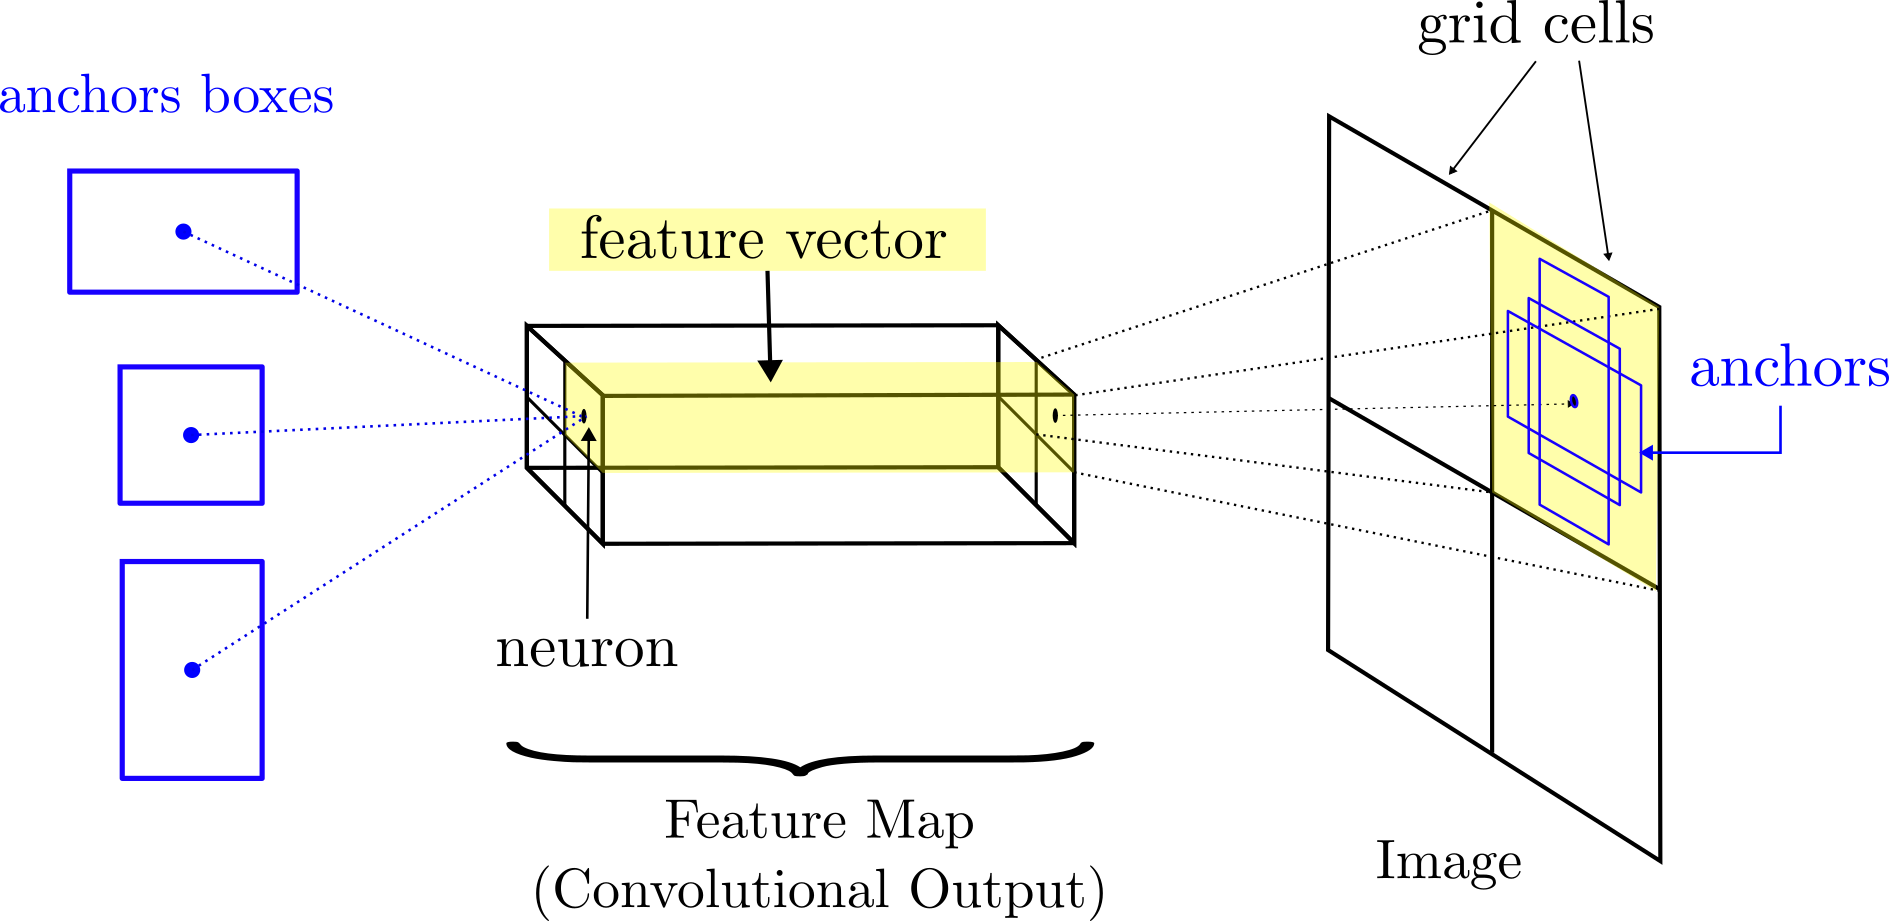
\includegraphics{figs/prep/anchor_box.png}
    \caption{\textbf{Illustration of the relationship between various terms used in one-stage object detection.}}
    \label{fig:explain_anchors}
\end{figure}

One-stage detection model learns to detect and classify objects using outputs from convolutional layers called \textit{feature maps}. Recall that convolutional layers preserve the spatial structure of the input data. For example, if an convolutional model produces a feature map of dimension $2 \times 2$ from an input image of size $256 \times 256$, then each of the four \textit{neurons} on the feature map corresponds with a $128 \times 128$ region on the input image, separating the image into $2 \times 2$ \textit{grid cells}.
In CNN models, multiple feature maps are produced simultaneously, thus each grid cell corresponds to a vector of output value called a \textit{feature vector}.

One-stage object detection models make use of a set of rectangular boxes called \textit{anchor boxes}. The dimensions of anchor boxes is fixed before training. When applied to grid cells, anchor boxes form \textit{anchors}, which are bounding boxes on the input image. Figure \ref{fig:explain_anchors} illustrates the relationship between different terms introduced. \textbf{A one-stage object detection model detects objects by learning to map anchors onto regions where an object is present.} During training, anchors which overlaps significantly with a labelled object is assigned to detect and classify the object. For detection, the model learns to produce the necessary values that transforms an anchor's bounding boxes to the bounding boxes of its assigned object. This is typically done by passing feature vectors through a deep neural network (DNN). For classification, a DNN is used in the same fashion to produce class probabilities.


\subsection{Supervised Contrastive Learning}
Contrastive learning refers to the technique of learning useful representations by bringing together positive example pairs and pushing apart negative example pairs in latent space. Contrastive learning often induces the learning of key differentiating features which are critical for downstream tasks such as classification.

Contrastive learning first found success in unsupervised learning, where works such as SimCLR \cite{chen_simple_2020} demonstrated its ability to learn useful features in the absence of labels.
The technique was first used in supervised learning by Khosla et al. \cite{khosla_supervised_2021}, which proposed using supervised label as a way to identify positive and negative example pairs. In a batch of training data, supervised contrastive loss maximises similarity between samples from the same class and minimises similarity between samples of different classes. Khosla et al. demonstrated that supervised contrastive loss can largely replace supervised loss for the task of image classification. Supervised contrastive loss has since been applied to natural language processing \cite{gunel_supervised_2021}, product matching \cite{peeters_supervised_2022} and affect modelling \cite{pinitas_supervised_2022}. However, there is very little existing work applying it to object detection. As far as I am aware, \textbf{this project represents first attempt to apply supervised contrastive learning for one-stage object detection,} and one of the first attempts for object detection in general.


\section{Task Analysis}
In this section, I analyse the risks of this project and how I planned to address them.

\subsection{Risks}
I planned to use the Cambridge High Performance Computing (HPC) cluster for model training and other computationally intensive parts of this project. This introduced several risks and here is how I tackled them:
\begin{enumerate}
    \item Learning curve of HPC
    \item Unforeseen bugs when running code on HPC, the difficulty of remote debugging
    \item Long queue time resulting in delay in project
\end{enumerate}
To mitigate the first factor, I read the HPC documentation and learnt through trial and error with small test jobs. To mitigate the second factor, I wrote unit tests for all critical components of the project. After every major change, I requested interactive sessions from the HPC cluster to test and debug in real time. These measures helped minimise wasted training time, which also mitigates the third factor. As a backup, I could train my model on my laptop or on a commercial compute platform like AWS Sagemaker.

\subsection{Software Engineering}

\subsubsection{Version Control}
I used Git for version control with a repository on GitHub. 
To backup my entire development environment, I used the Windows utility \verb|FreeFileSync| to synchronise it weekly with a copy on Google Drive.


\subsubsection{Tests}
\begin{wrapfigure}{l}{0.5\textwidth}
    \centering
    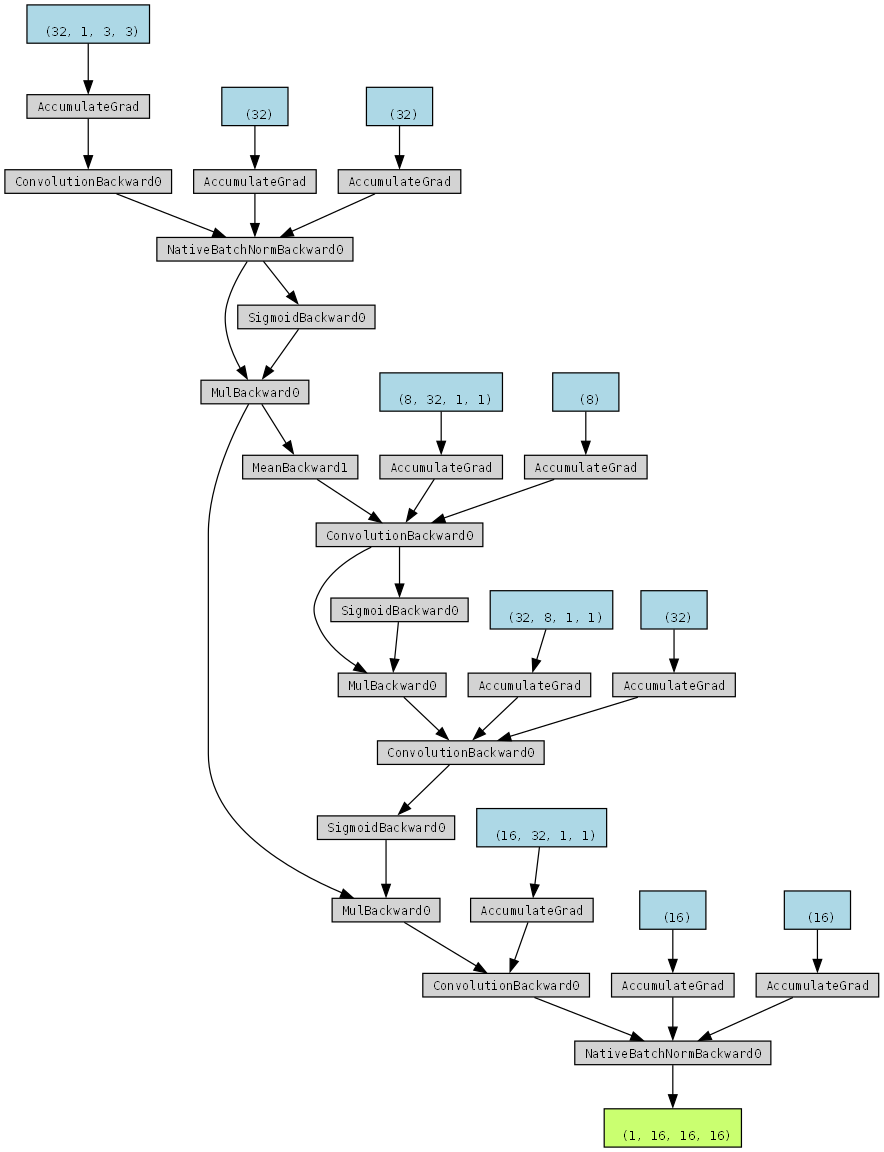
\includegraphics[width=0.5\textwidth]{figs/prep/torchviz_example.png.png}
    \caption{\textbf{Visualisation of \texttt{MBConvBlock}}, a component of EfficientNet \cite{tan_efficientnet_2020}}
    \label{fig: mbconvblock}
\end{wrapfigure}
For components of the project where there are expected input-output pairs, such as loss functions, evaluation algorithms, and the output size of ML models, I wrote unit tests using the library \verb|pytest|. Using GitHub Actions I ensured that unit tests were run after each commit to ensure a basic level of continuous integration. 

However, many aspects of this project proved to be difficult to test with unit tests alone. ML models are difficult to test because there is no way of knowing the correct output. To overcome this, I visualised the model execution graphs using the library \verb|torchviz| and manually inspected for errors (Figure \ref{fig: mbconvblock} shows an example of such visualisation). I also found the library \verb|fvcore| helpful as it helps to detect unused model weights, which helped to catch accidental typos in the model code. When available, I also tested models by loading open source pre-trained weights from other implementations of the same model. This helps to ensure that the components of the model are of the correct dimensions.


\subsubsection{Language \& Frameworks}
I wrote the project in Python as it is the language of choice for machine learning tasks. I chose to build my deep learning models on PyTorch, as it has excellent documentation, community support, and a suite of debugging tools. For computer vision related tasks, I used both OpenCV and Pillow, as I needed different features from them. For hyperparameter tuning, I chose Optuna as it is well-documented, light-weight, and followed the features I needed.


\section{Past Experience}
Prior to this project, I had used Python extensively for years and was comfortable with the language. For object detection, I had used a command-line utility to train an object detection model in TensorFlow. I did so as part of a summer internship. The utility only required a rudimentary understanding of basic data loading and there was hardly any coding involved. Outside of this, 
my previous experience with machine learning frameworks was limited to completing TensorFlow and PyTorch tutorials.

\chapter{Implementation}
\section{Repository Overview}
The code structure of this project is as follows:
\begin{center}
    \begin{forest}
      for tree={
        font=\ttfamily,
        grow'=0,
        child anchor=west,
        parent anchor=south,
        anchor=west,
        calign=first,
        inner xsep=7pt,
        edge path={
          \noexpand\path [draw, \forestoption{edge}]
          (!u.south west) +(7.5pt,0) |- (.child anchor) pic {folder} \forestoption{edge label};
        },
        % style for your file node 
        file/.style={edge path={\noexpand\path [draw, \forestoption{edge}]
          (!u.south west) +(7.5pt,0) |- (.child anchor) \forestoption{edge label};},
          inner xsep=2pt,font=\small\ttfamily
                     },
        before typesetting nodes={
          if n=1
            {insert before={[,phantom]}}
            {}
        },
        fit=band,
        before computing xy={l=15pt},
      }  
    [marine-organism-detector
      [efficientnet]
      [efficientdet]
      [yolite
        [train\_yolite.py,file]
        [tune\_yolite.py,file]
      ]
      [exgen
        [gan\_models]
        [exgen.py, file]
      ]
      [utils]
      [dataset]
      [tests]
      [training]
      [train.py,file]
      [tune.py,file]
      [video\_detector.py,file]
    ]
\end{forest}
\end{center}
\begin{itemize}
    \item \verb|efficientnet|, \verb|efficientdet| and \verb|yolite| contains my implmentations of models EfficientNet \cite{tan_efficientnet_2020}, EfficientDet \cite{tan_efficientdet_2020} and Yolite, which is proposed in this project
    \item \verb|exgen| contains the training example generator, which can be ran with \verb|exgen.py|
    \item \verb|dataset| contains code for data loading and manipulation
    \item \verb|tests| contains unit tests
    \item \verb|utils| contains useful functions for the entire project
    \item \verb|train.py| and \verb|tune.py| runs distributed training and hyperparameter tuning. They share many functions that are stored in \verb|training|. 
\end{itemize}

All code listed was written from scratch. 

\section{Dataset}
The project used a subset of the FathomNet \cite{katija_fathomnet_2022} dataset, an open-source collection of annotated marine organism images. As of November 2022, it contained 84,454 images and 175,958 annotations. Each image in the dataset is annotated with creatures it contains, each creatures has a bounding box that describes its position in the image, as well as its biological concept. Biological concepts are part of FathomNet's unique hierarchical class structure, which mirrors the phylogeny tree of marine creatures. This allows creatures to be labelled at different levels of granularity. For example, if the specific species of a creature if known, then it can be labelled exactly. If it is unknown, the creature could still be labelled by a wider classification such as \textit{Asteroidea}, a class that contains all starfishes.

\subsection{Classification}
I started by identifying a subset of the FathomNet dataset relevant to this project and classifying these examples into classes for classification. To facilitate this, it would be very useful as reference to have a tree of biological concepts in FathomNet and the number of annotations available for each biological concept. The team behind FathomNet did release a python library which should help with this task, but I found that the concept tree retrieved this way was extremely sparse as it exhaustively included all biological concepts available, including hundreds of thousands for each FathomNet has no training example. To work around this, I realised that the FathomNet website allows users to browse a subset of the concept tree that only included concepts for which there were valid training examples, which was exactly what I needed. I inspected the http requests made by the website and managed to derive a way to download this tree.

With this concept tree in hand, I worked with Dr Emily Mitchell to identified concepts relevant to the project and classified them into 11 classes. Table \ref{table:class_breakdown} shows a breakdown of this classification. 
\begin{table}[H]
    \begin{center}
        \begin{tabular}{||c c c||}
            \hline
             \textbf{Class} & \textbf{\#Training Examples}  & \textbf{\#Testing Examples} \\
             \hline
             \hline 
             Stony corals   & 95    &   10\\
             Black corals   & 108   &   37\\
             Demosponges    & 763   &   200\\
             Glass sponges  & 2191  &   716\\
             Sea pens       & 2303  &   705\\
             Sea cucumbers  & 4818  &   1257\\
             Starfish       & 5234  &   1544\\
             Sea anemones   & 5913  &   1667\\
             Soft corals    & 6188  &   1803\\
             Sea pigs       & 6537  &   1811\\
             Sea urchins    & 10323 &   2911\\
             \hline
             \hline
             \textit{Total} & 44473 &  13376\\
             \hline
        \end{tabular}
    \caption{\label{table:class_breakdown} Overview of initial classes and the number of examples. The class are sorted in ascending order by the total number of available examples.}
    \end{center}
\end{table}

Worth noting is the shortage of examples for the classes of stony corals and black corals, for which I have around 100 examples. In comparison, I have well over 13,000 examples of sea urchins, the most numerous class. Keeping both classes in its current state would leave a severe class imbalance in the dataset, which would be a major obstacle to classification training. For this project, I mitigated the effect of this imbalance through dynamic example generation, which I detail in \ref{section: exgen}.

\subsection{Retrieval and Cleaning}
My subset of FathomNet contained 25,093 images, requiring around 64 Gigabyte of storage. With 8 threads downloading from the server in parallel, I was able to retrieve all images in less than 2 hours. The process was smooth. The FathomNet dataset did not provide its annotation in a standard format, hence I converted and stored all annotations in the popular Pascal VOC format \cite{}.

\begin{figure}[H]
    \begin{subfigure}[b]{0.45\textwidth}
        \centering
        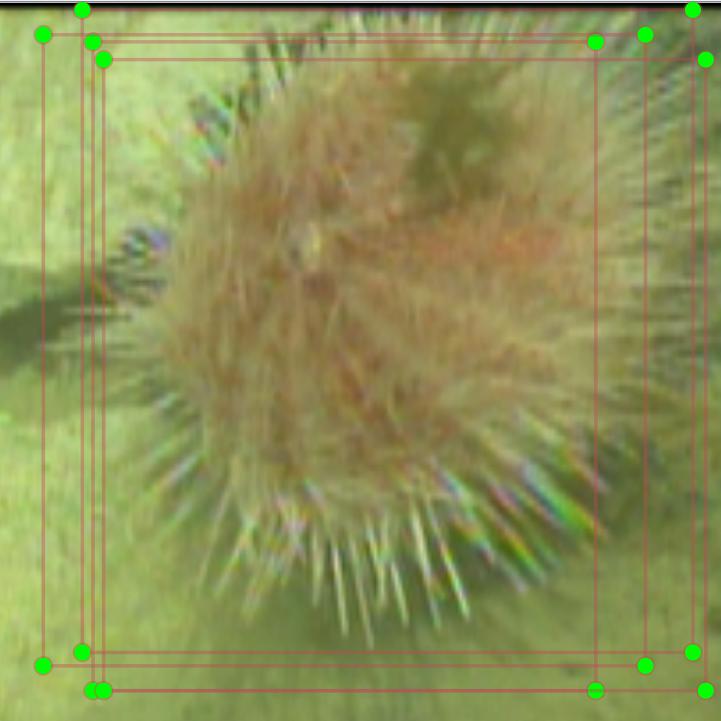
\includegraphics[width=\textwidth]{figs/implementation/fathomnet_problems/duplicate.png}
        \subcaption{\textbf{Duplicated Annotations}}
        \label{fig:fathomnet_duplicate}
    \end{subfigure}
    \hfill
    \begin{subfigure}[b]{0.45\textwidth}
        \centering
        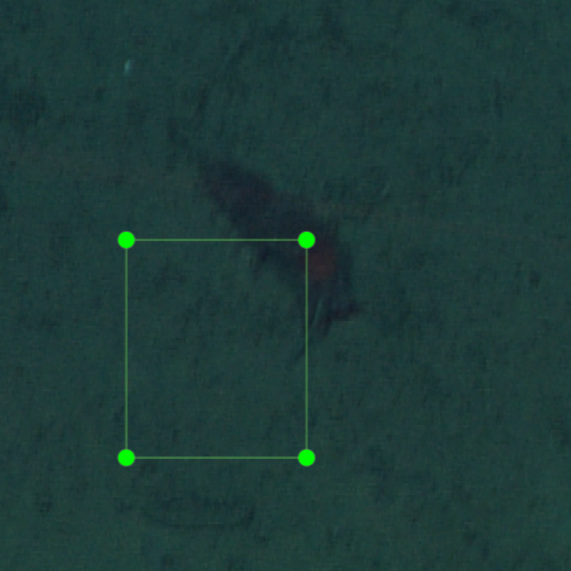
\includegraphics[width=\textwidth]{figs/implementation/fathomnet_problems/inaccurate.png}
        \subcaption{\textbf{Inaccurate Annotation}}
        \label{fig:fathomnet_inaccurate}
    \end{subfigure}
    \hfill
    \begin{subfigure}[b]{0.45\textwidth}
        \centering
        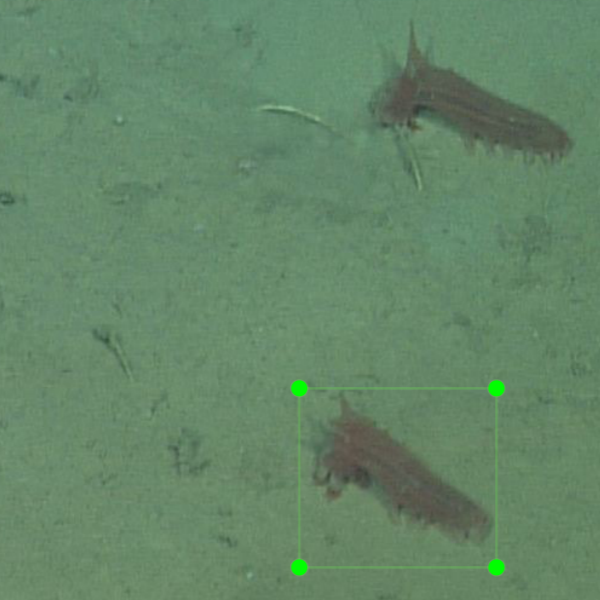
\includegraphics[width=\textwidth]{figs/implementation/fathomnet_problems/missing.png}
        \subcaption{\textbf{Missing Annotation}}
        \label{fig:fathomnet_missing}
    \end{subfigure}
    \hfill
    \begin{subfigure}[b]{0.45\textwidth}
        \centering
        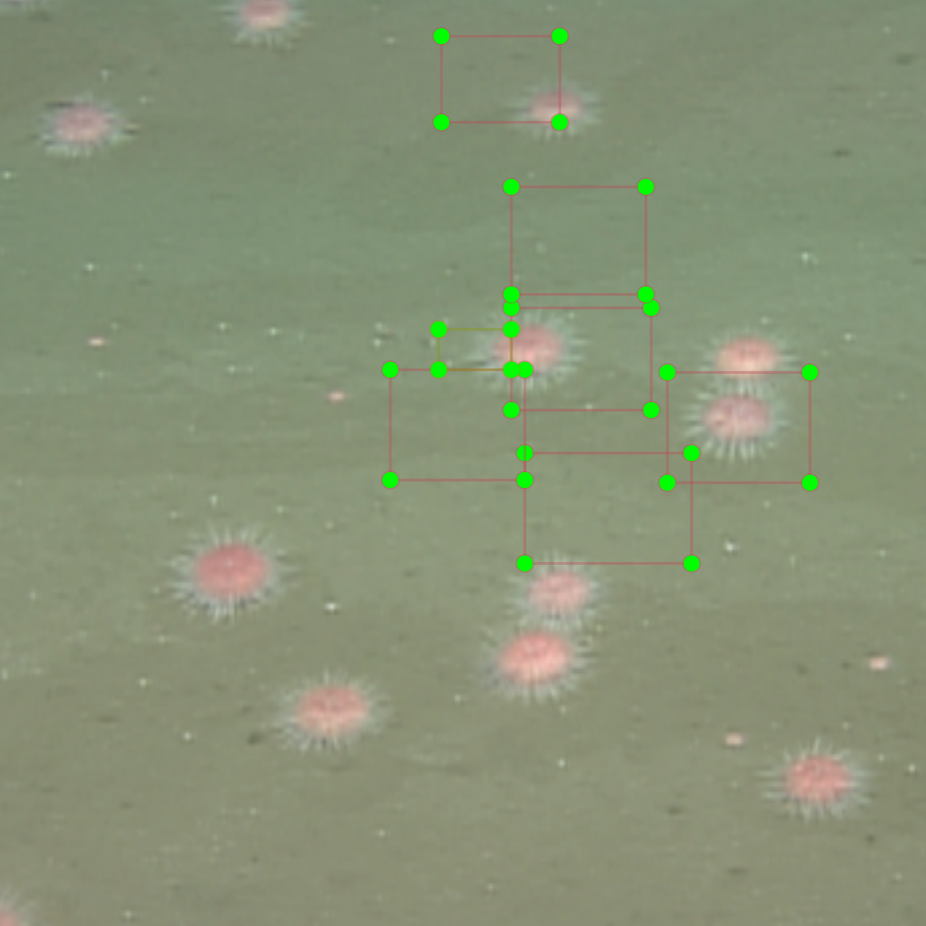
\includegraphics[width=\textwidth]{figs/implementation/fathomnet_problems/incorrect.png}
        \subcaption{\textbf{Incorrect Annotations}}
        \label{fig:fathomnet_incorrect}
    \end{subfigure}
    
    \caption{\textbf{Examples of problems with the FathomNet dataset.} To ensure I was not ``cherryicking'', all the examples were found within the first 40 images of the dataset.}
    \label{fig:fathomnet_problems}
\end{figure}

I proceeded to inspect and clean the dataset, \textbf{which revealed a generally poor quality of annotations}. Even a quick inspection revealed frequent instances of duplicated annotations (Figure \ref{fig:fathomnet_duplicate}), inaccurate annotations (Figure \ref{fig:fathomnet_inaccurate}) and missing annotations (Figure \ref{fig:fathomnet_missing}). Some images have many incorrect annotations (Figure \ref{fig:fathomnet_incorrect}). Amongst these problems, only duplicated annotation could be removed computationally; I removed them by ordering annotation in each image and removing all annotations which shares a $>90\%$ overlap with an earlier annotation. Inaccurate and missing annotations both required tedious manual inspection and cleaning. I did not proceed with manual cleaning for two reasons:
\begin{enumerate}
    \item The large number of images meant this would take a long time;  the limited time for the project is better spent on extending its more technical aspects,
    \item I lacked the expert knowledge to correct many of the missing annotations
\end{enumerate}

\subsection{Data Augmentation} \label{section: data_aug}
Object detection models require that the data augmentation techniques either preserve the locations of annotated bounding boxes or translate them into the correct positions. With these in mind, I developed the following data augmentation techniques: 

\subsubsection{Rotation}
\begin{figure}[H]
    \centering
    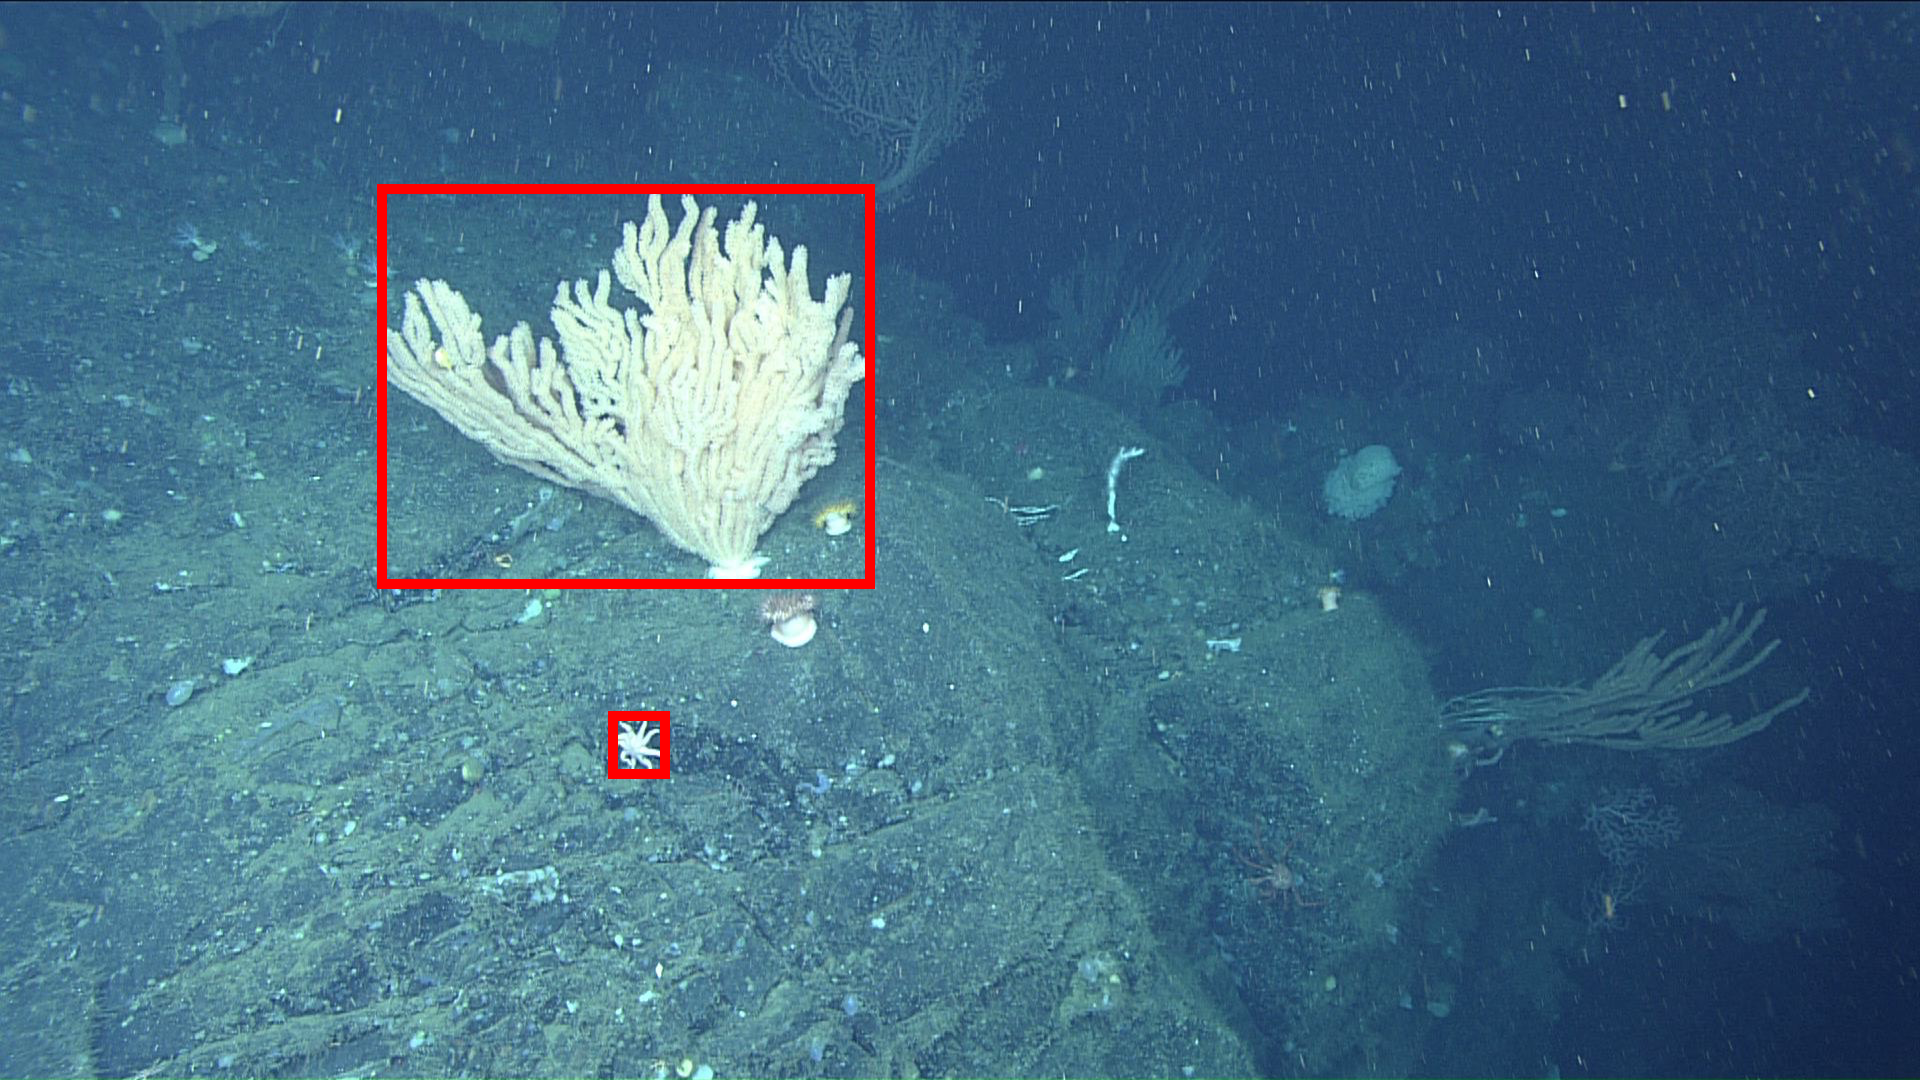
\includegraphics[width=0.45\textwidth]{figs/implementation/aug/before.png}
    \hfill
    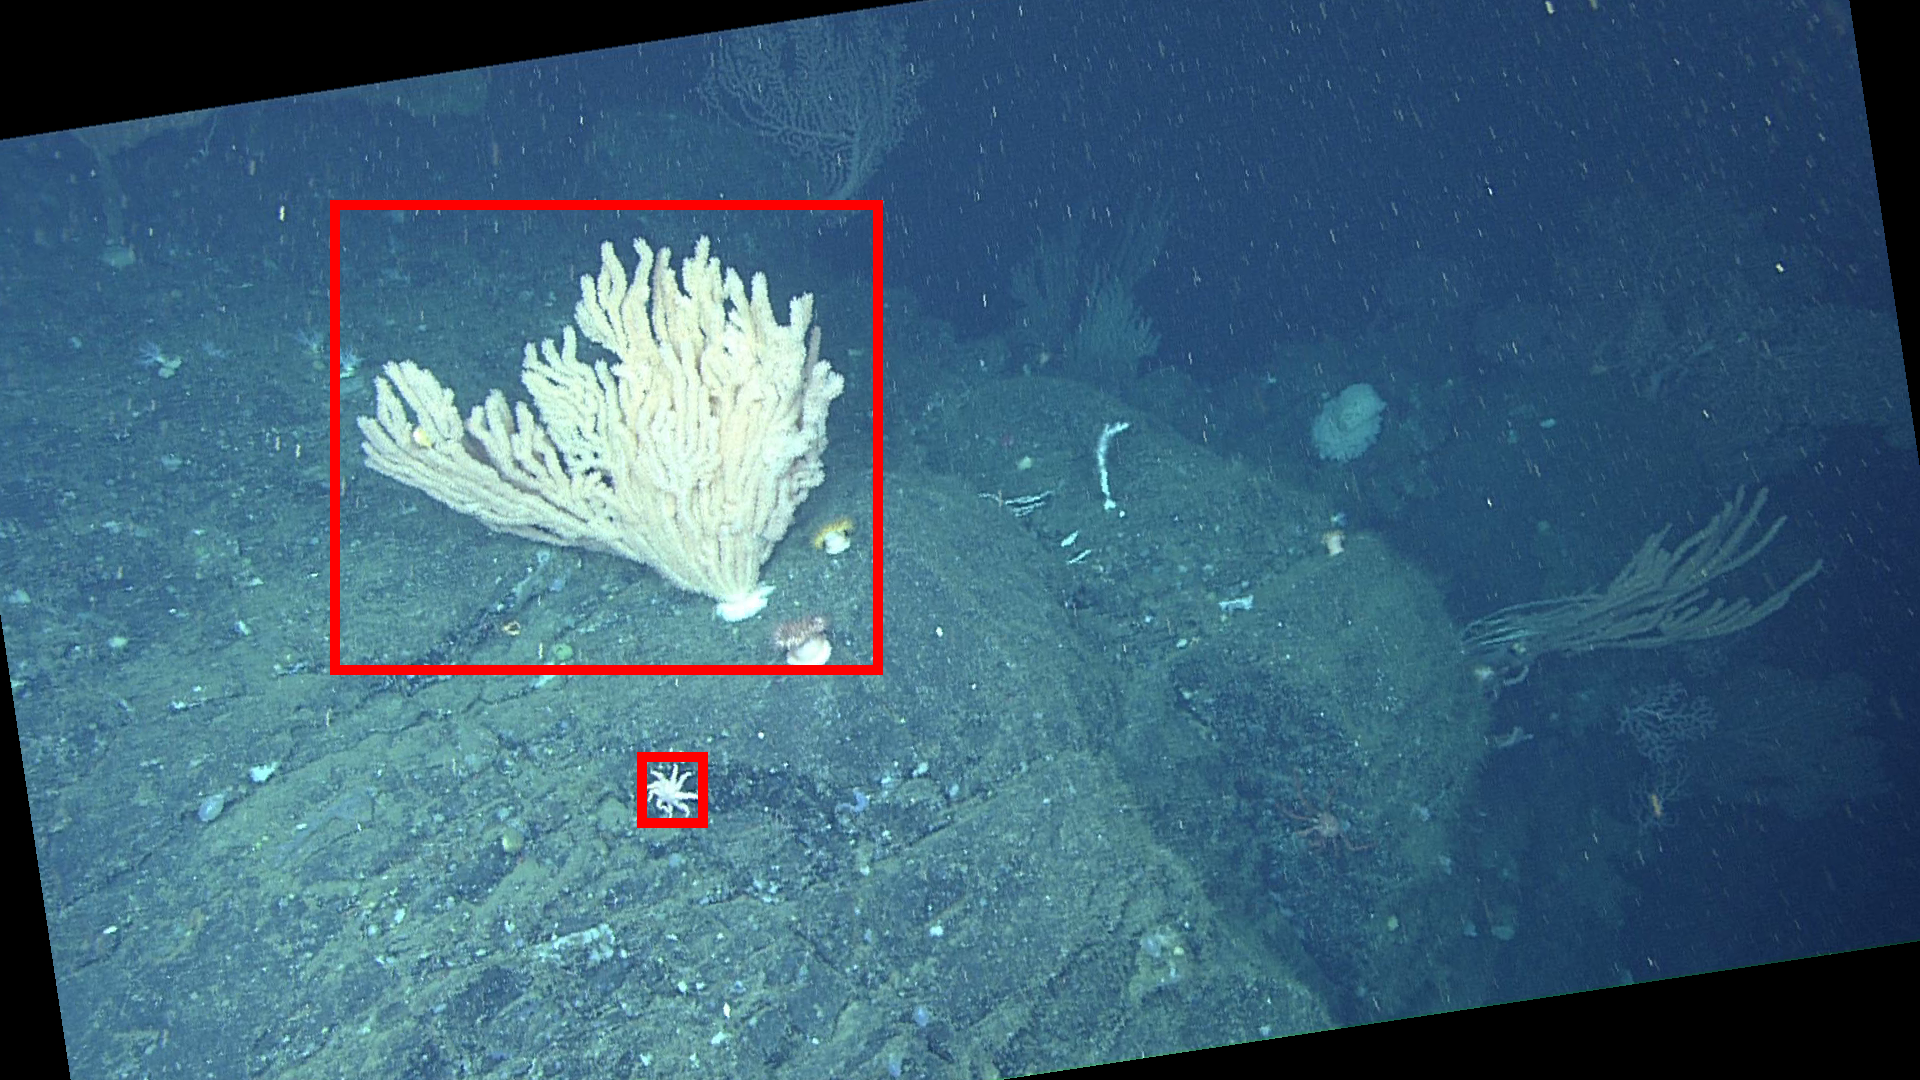
\includegraphics[width=0.45\textwidth]{figs/implementation/aug/rot.png}
    \caption{\textbf{Left: Original image. Right: After rotation}}
    \label{fig:aug_rotate}
\end{figure}
I applied an rotation of up to $25\deg$ clockwise/anti-clockwise on each input image. Annotation bounding boxes were transformed with matrix multiplications.
{
\subsubsection{Horizontal Flip}
\begin{figure}[H]
    \centering
    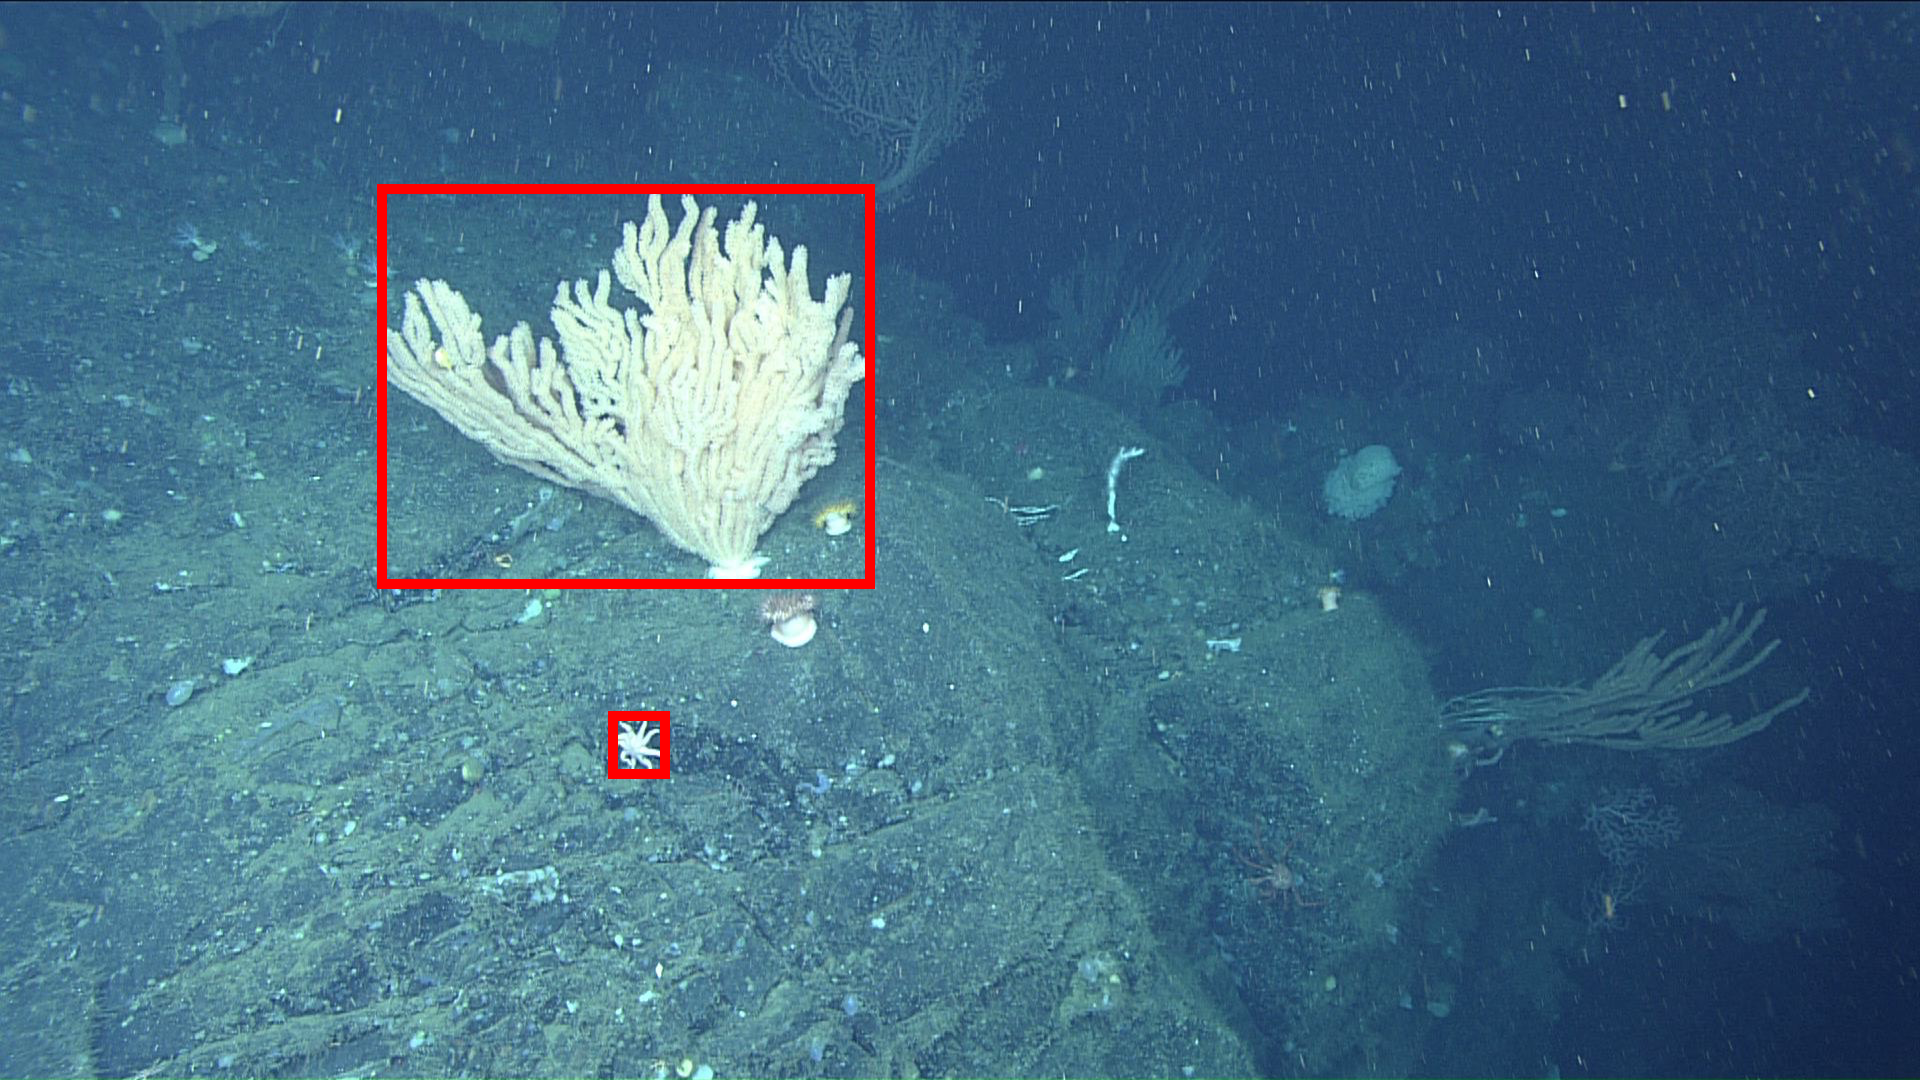
\includegraphics[width=0.45\textwidth]{figs/implementation/aug/before.png}
    \hfill
    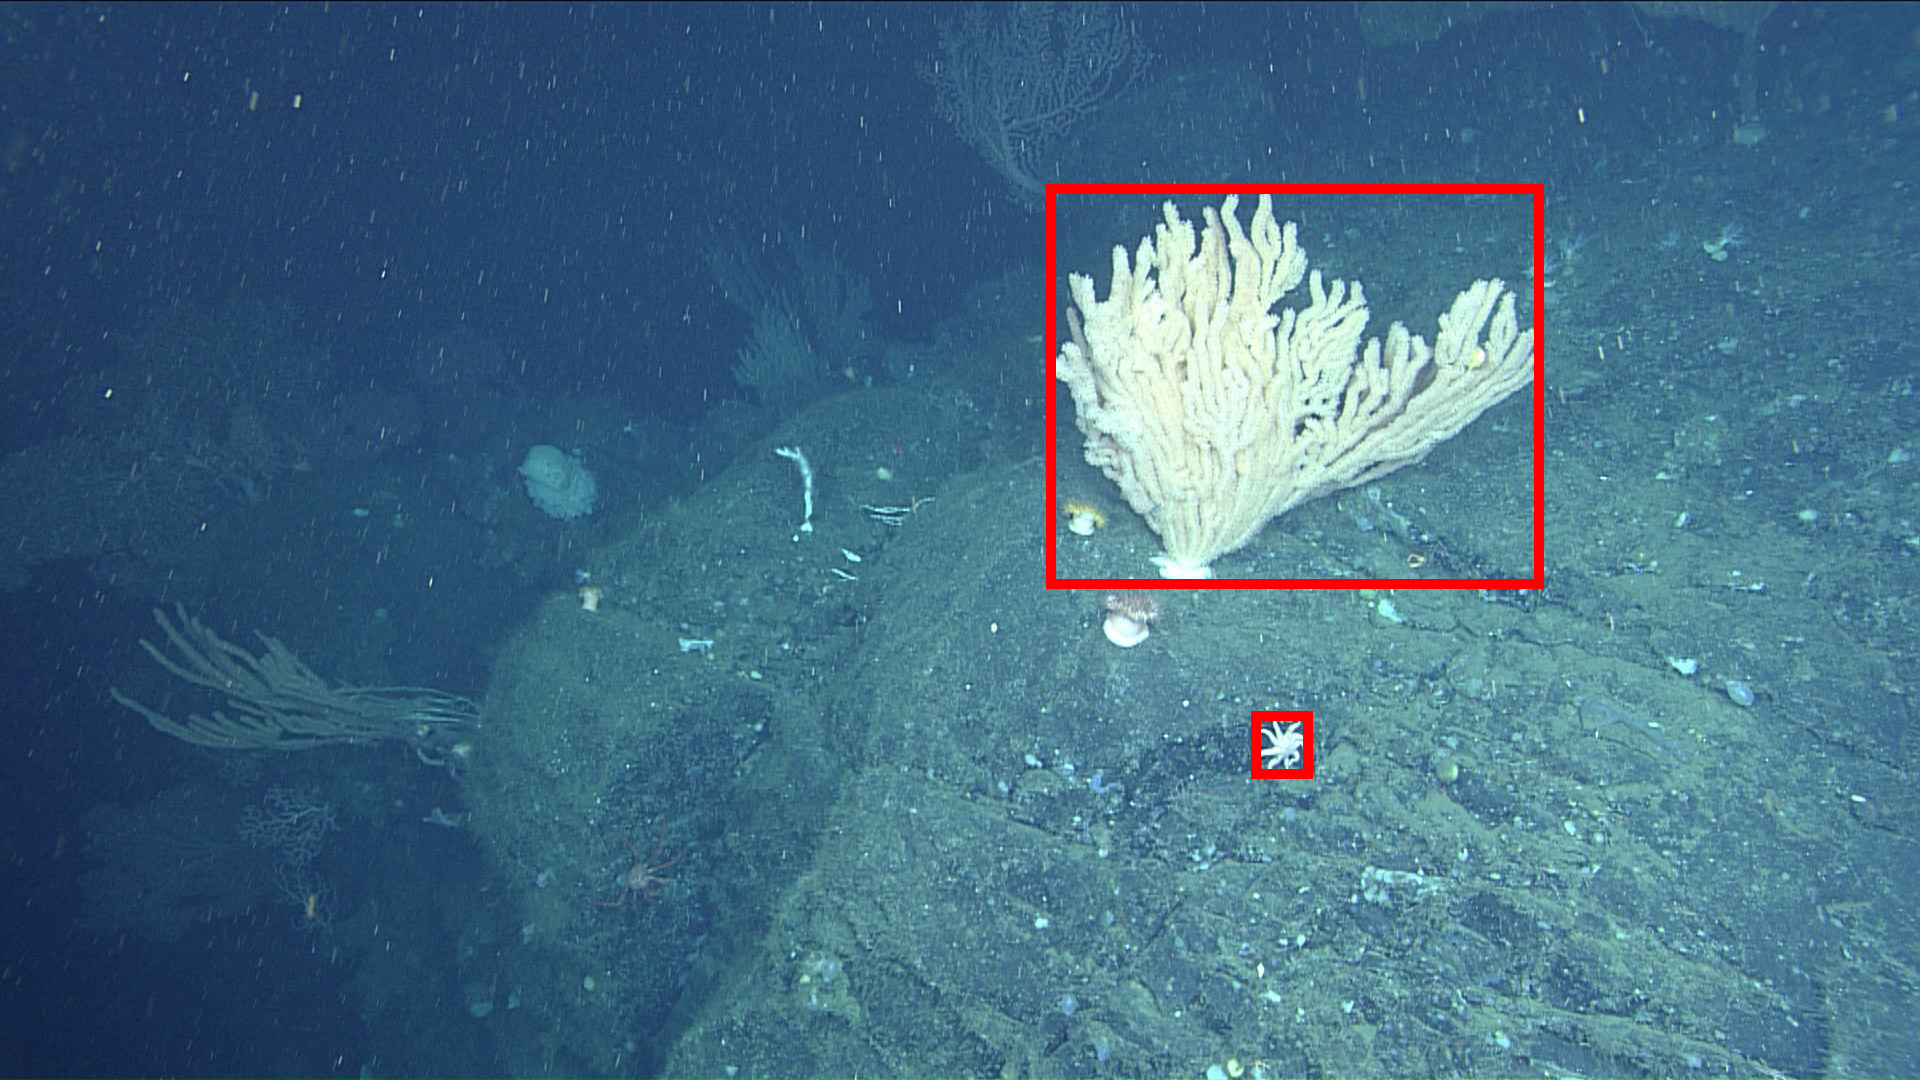
\includegraphics[width=0.45\textwidth]{figs/implementation/aug/flip.png}
    \caption{\textbf{Left: Original image. Right: After horizontal flipping}}
    \label{fig:aug_flip}
\end{figure}
This augmentation randomly performs a horizon flip. Since virtually all organisms in the dataset is left-right symmetric, I applied this transform 50\% of the time to ensure an equal portion of flipped and non-flipped examples.
}

\subsubsection{Gaussian Noise}
\begin{figure}[H]
    \centering
    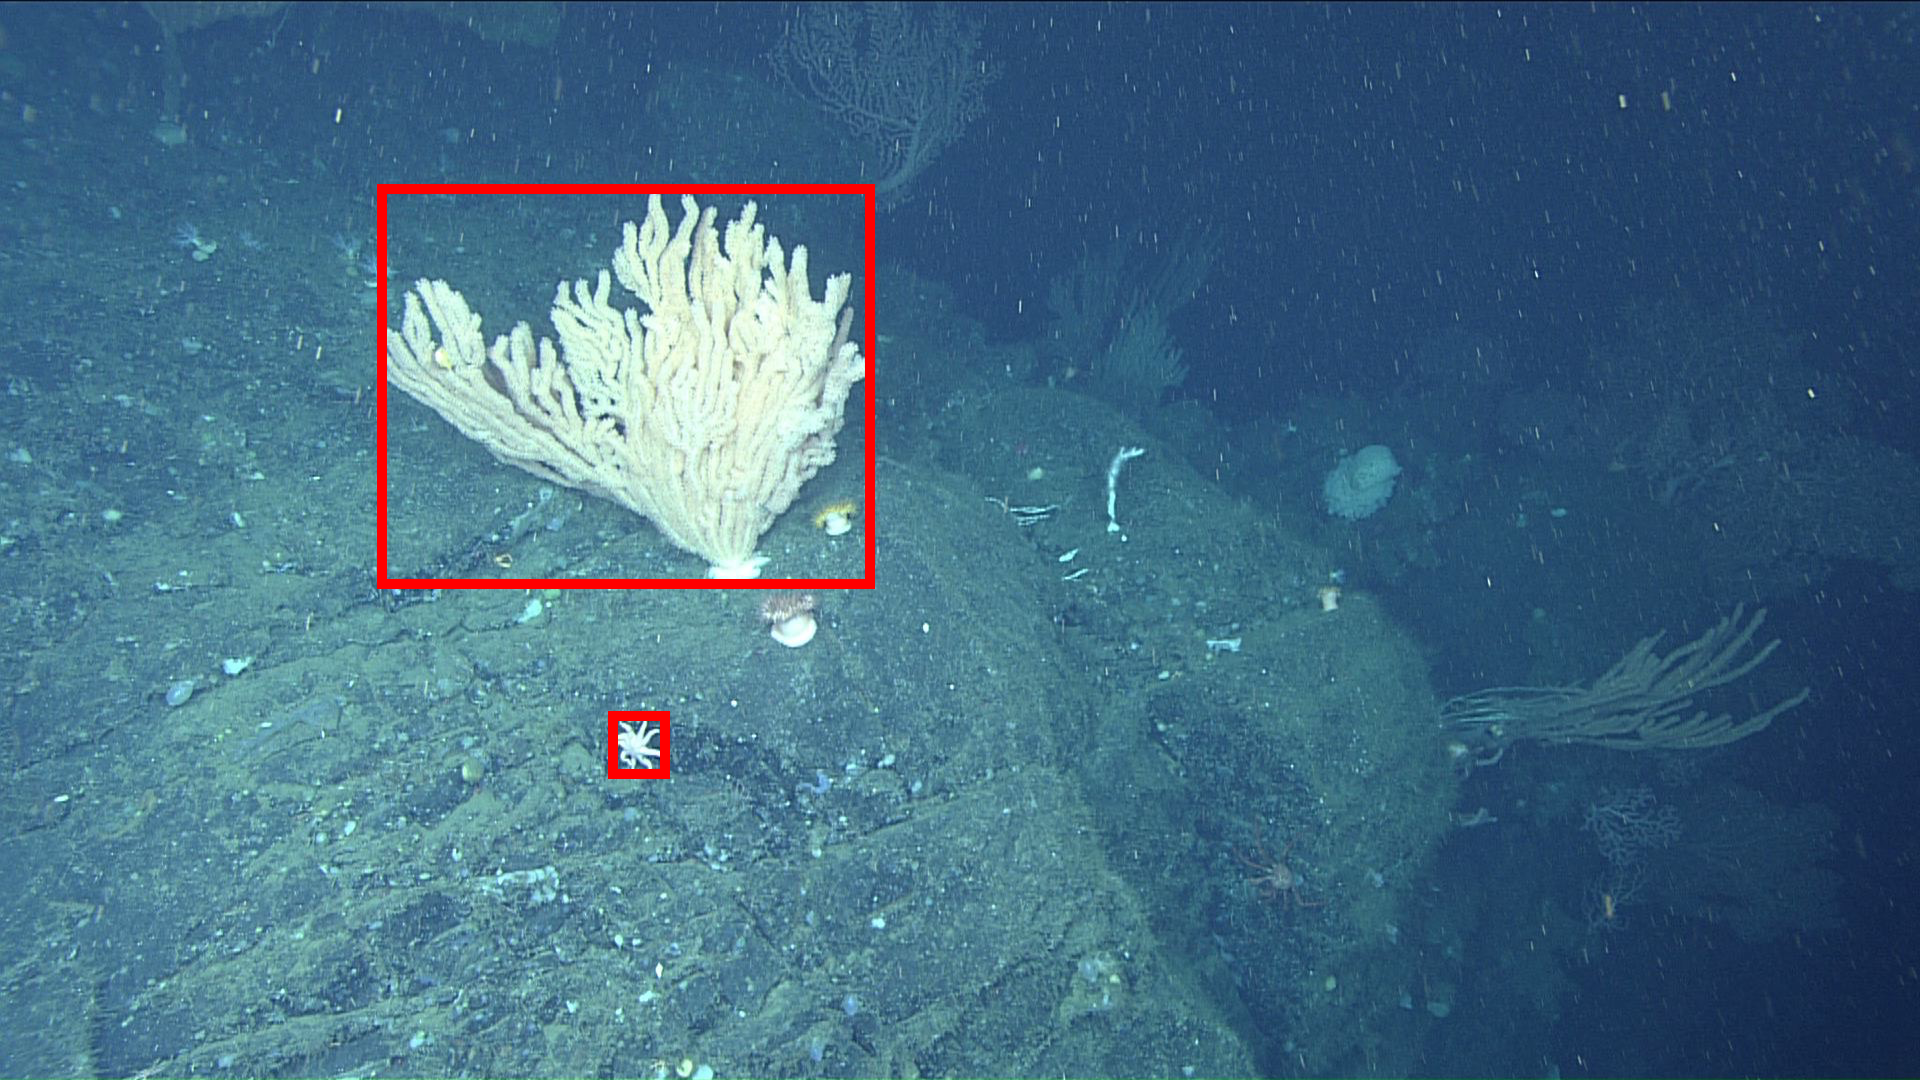
\includegraphics[width=0.45\textwidth]{figs/implementation/aug/before.png}
    \hfill
    \includegraphics[width=0.45\textwidth]{figs/implementation/aug/noise.png}
    \caption{\textbf{Left: Original image. Right: After adding Gaussian noise}}
    \label{fig:aug_noise}
\end{figure}
This augmentation adds a random noise to each pixel of the input image, with the noise sampled from a Gaussian distribution.

\subsubsection{Random Erasing}
\begin{figure}[H]
    \centering
    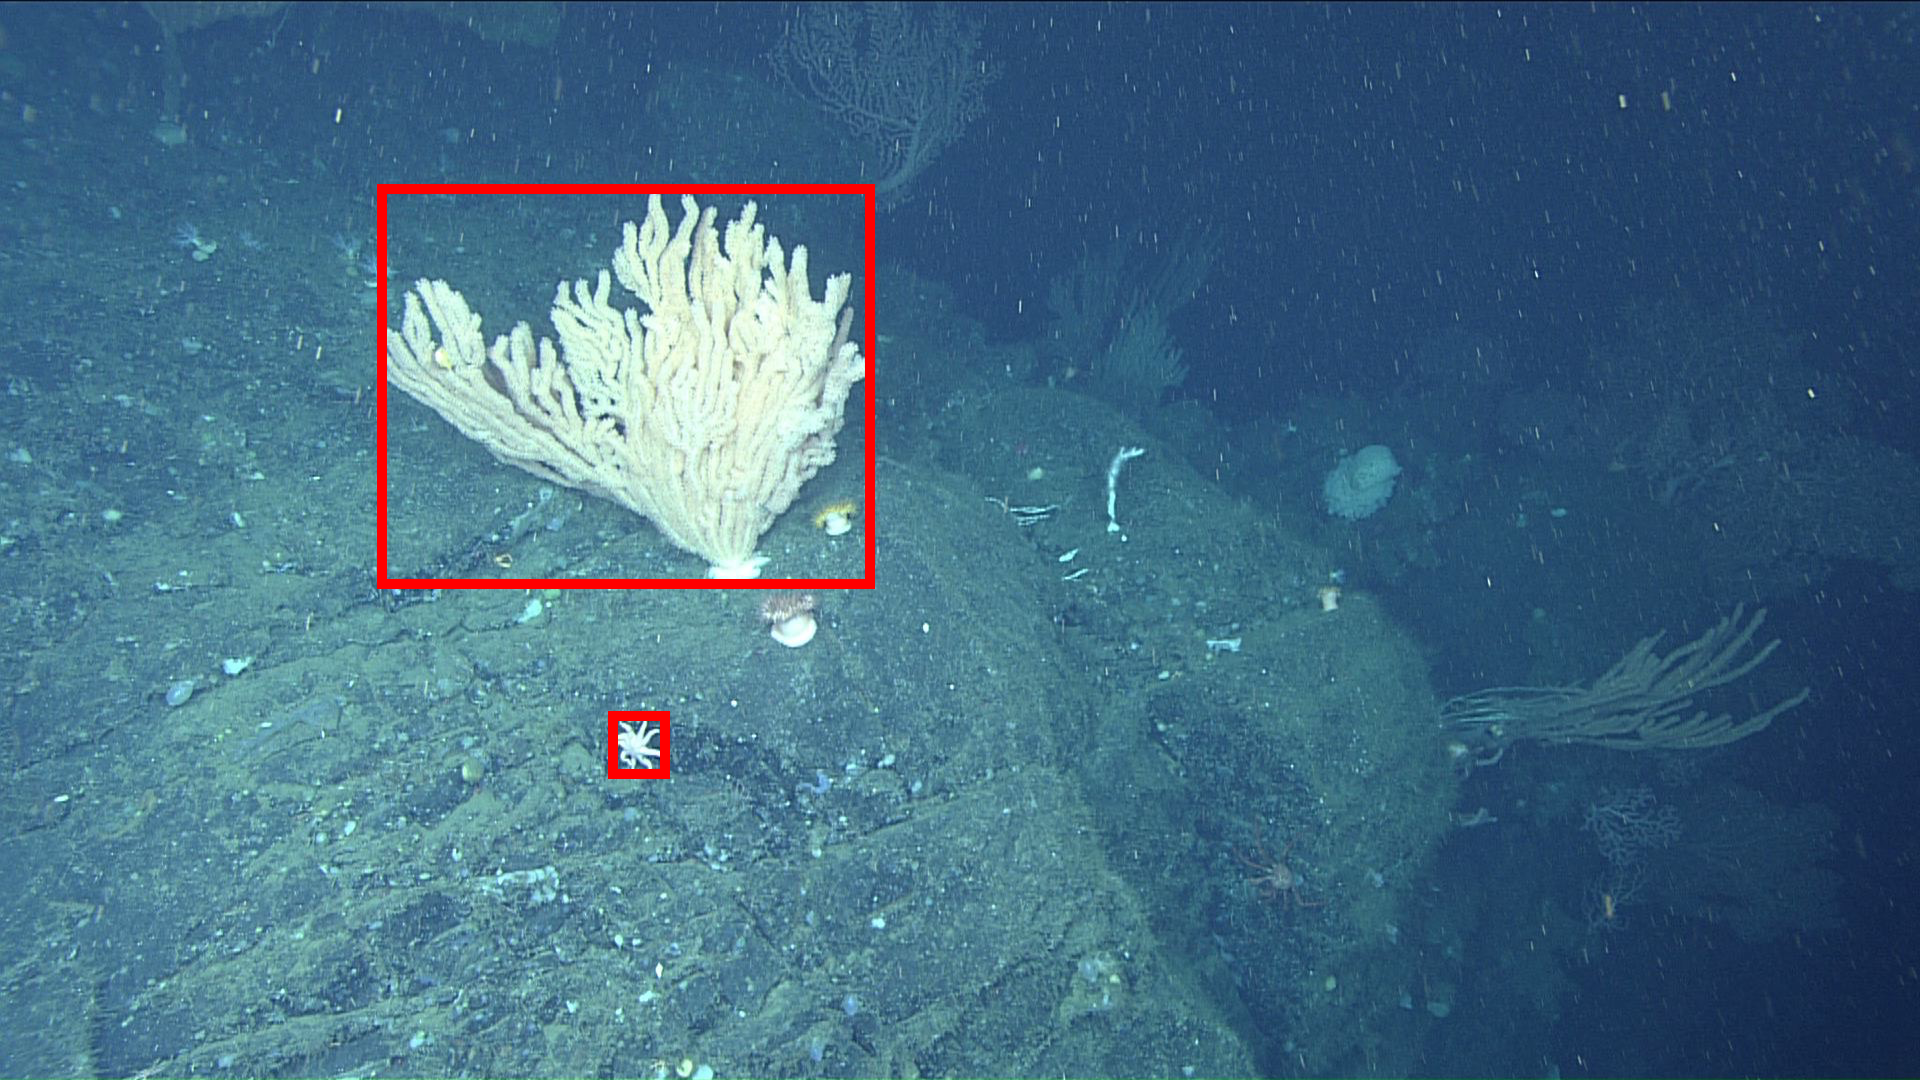
\includegraphics[width=0.45\textwidth]{figs/implementation/aug/before.png}
    \hfill
    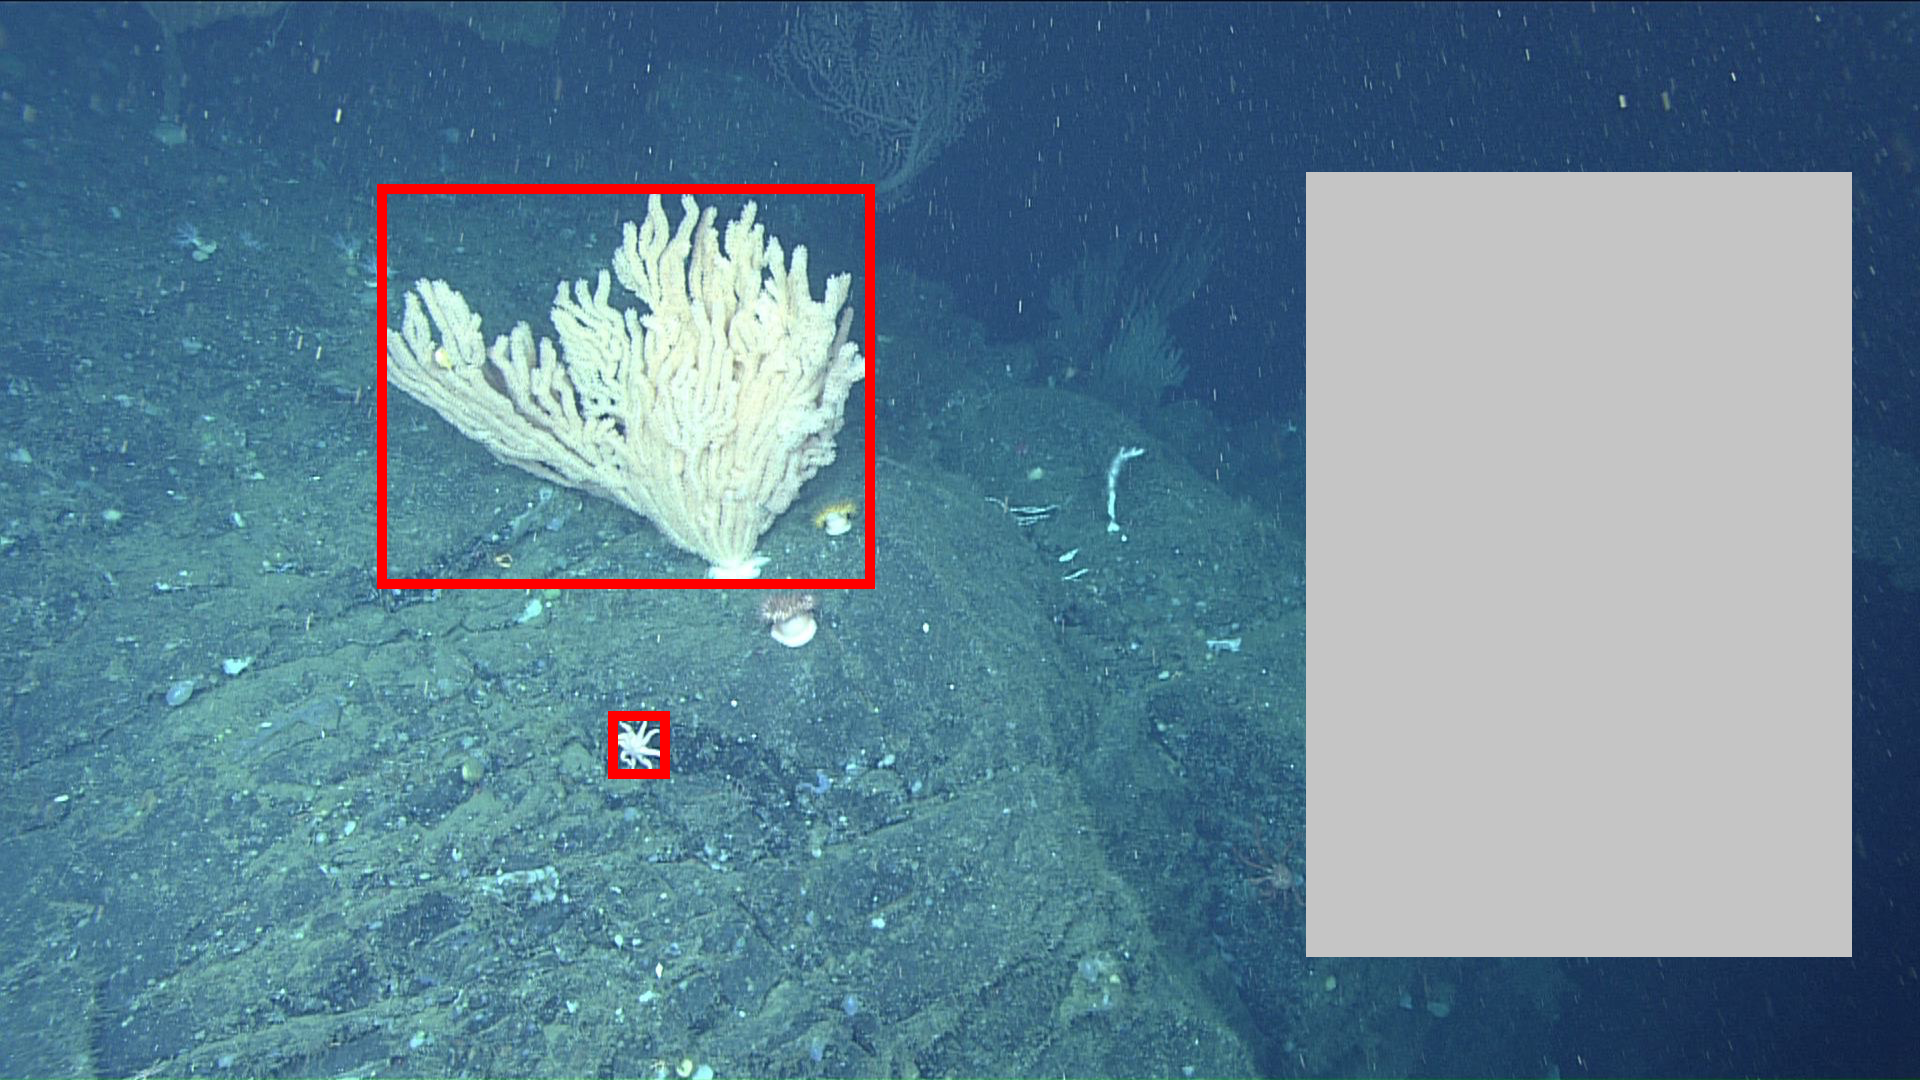
\includegraphics[width=0.45\textwidth]{figs/implementation/aug/erase.png}
    \caption{\textbf{Left: Original image. Right: After random erasing}}
    \label{fig:aug_erase}
\end{figure}
Proposed Zhong et al.\cite{zhong_random_2017}, I implemented this technique from scratch based on the descriptions in the paper.
I did not remove any annotation even if its bounding box was fully erased.
In practise, I only enabled this augmentation on 10\% of all inputs due to its large impact on training data.

\subsubsection{Pixel Jittering}
\begin{figure}[H]
    \centering
    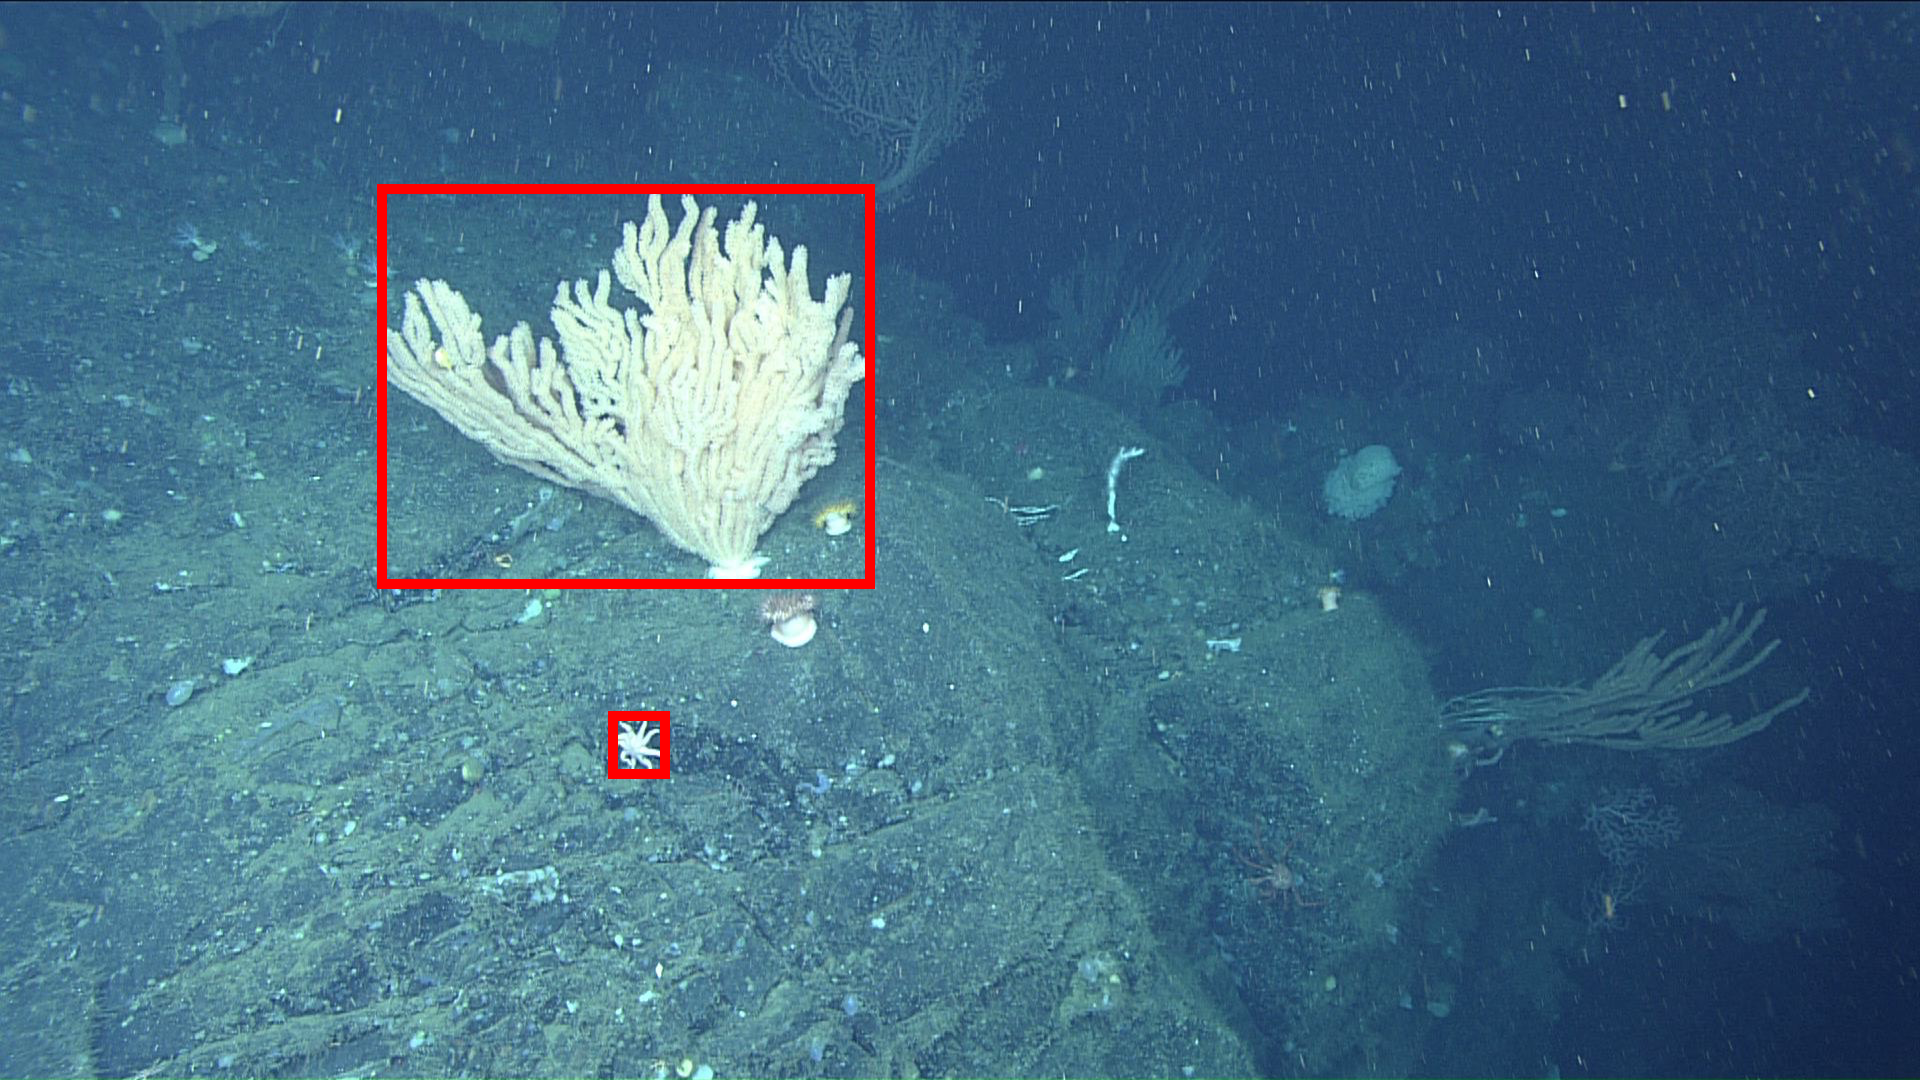
\includegraphics[width=0.45\textwidth]{figs/implementation/aug/before.png}
    \hfill
    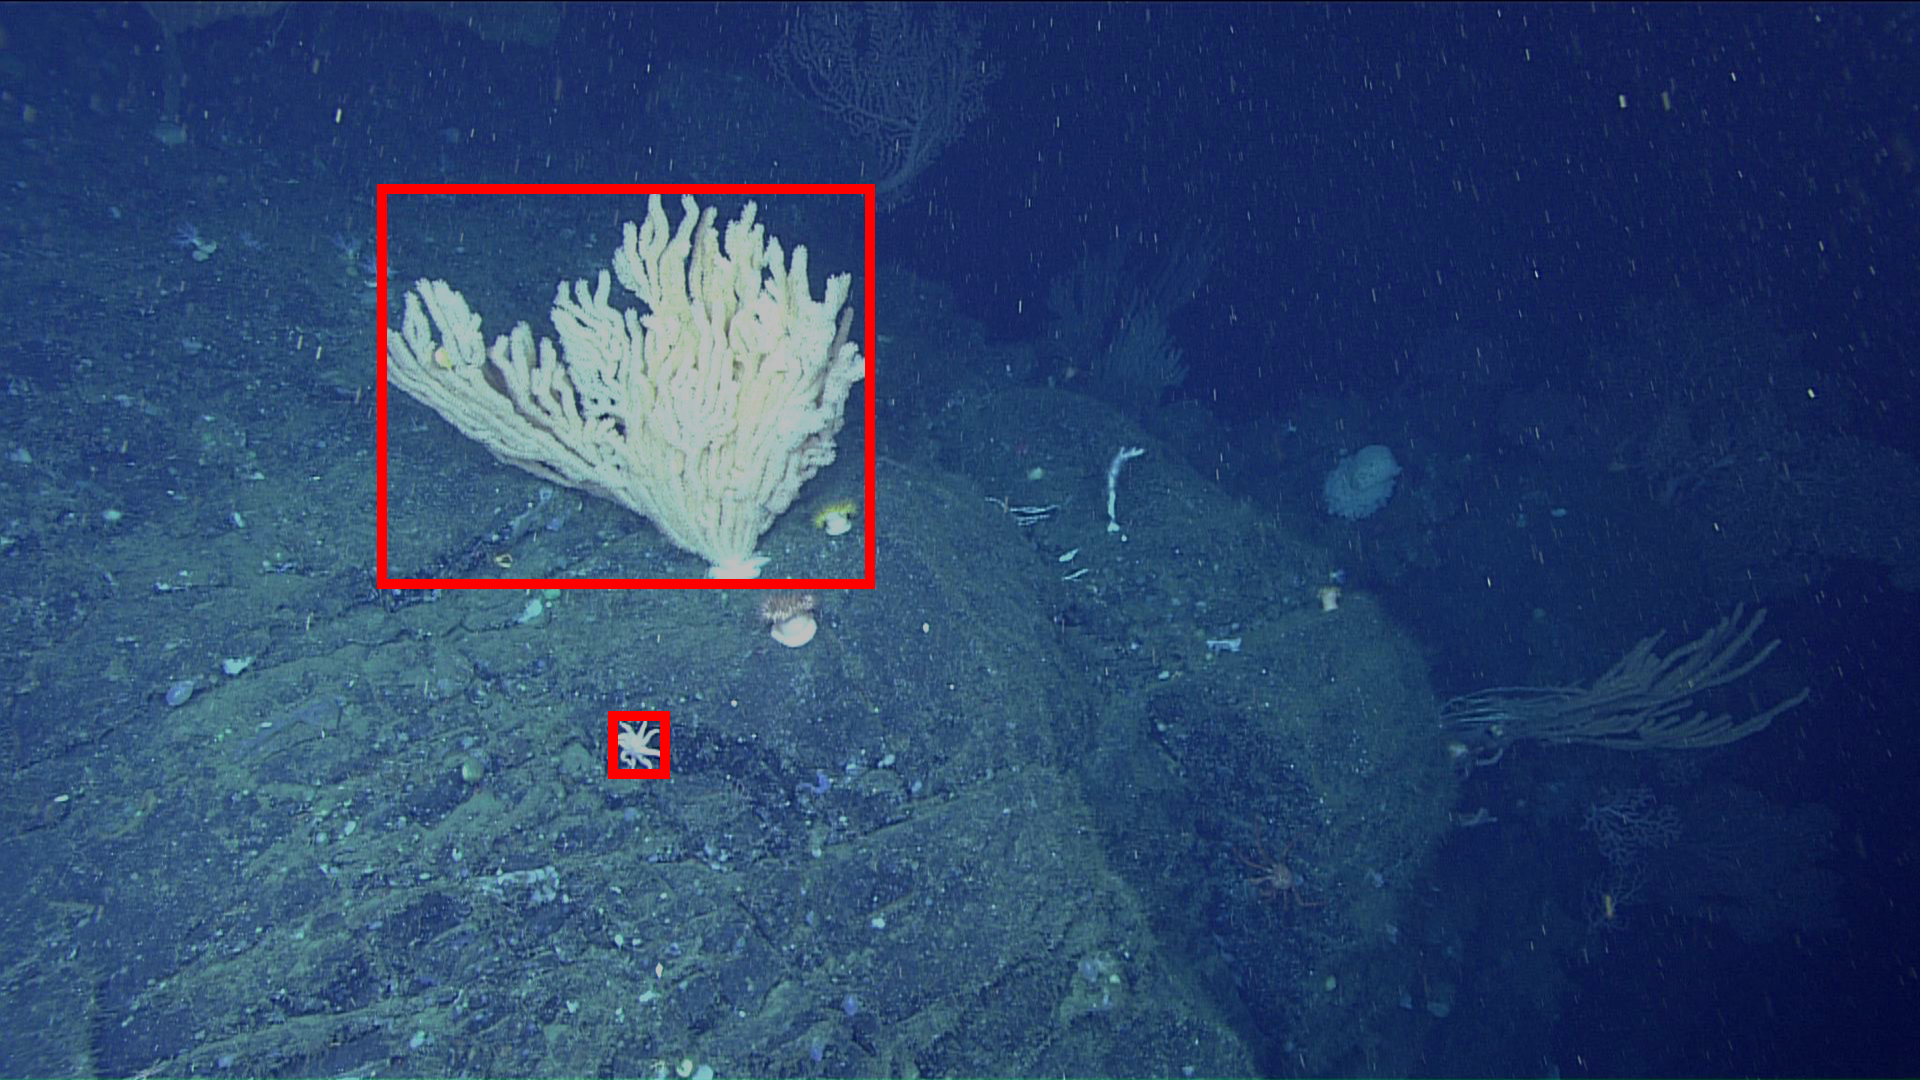
\includegraphics[width=0.45\textwidth]{figs/implementation/aug/jitter.png}
    \caption{\textbf{Left: Original image. Right: After pixel jittering}}
    \label{fig:aug_jitter}
\end{figure}
This augmentation randomly modifies the brightness, contrast, hue and saturation values of the input image. For this project, this helps to emulate the varied lighting conditions in underwater footage.
\section{Training Example Generator} \label{section: exgen}
In this section, I will detail my implementation process of the dynamic training example generator, a key requirement of my project. The goal of the training example generator is to create new training examples from existing data.

\subsection{Motivations}
The need for a training example generator became apparent with the severe class imbalance of FathomNet. As described previously, a shortage in training examples could have prevented the inclusion of some important classes of marine animals, such as black corals and stony corals. Fine-grained classification, such as differentiating between different families of sea urchins, was also hindered as the effect of example shortage and class imbalance became more severe. It was clear that some way of generating new training examples were needed to overcome the limitations of training data.

Another motivation for the training example generator relates to the specific difficulty of working with sessile benthic animals. Many of these creatures have soft bodies of complex, irregular shapes. As a result, their appearance varies significantly based on time, perspective and the environment. Representing these variations required a large amount of training data that was unavailable, thus models tend to overfit. However, we can partially mitigate this issue by deliberately transform individual creatures in the dataset. By choosing transformations suitable for each class of creatures, we can emulate visual variation from a small set of training examples. Data augmentation is widely used in machine learning as a way to achieve generalisability. By applying augmentations to individual creatures, the training example generator includes a data augmentation technique specific for object detection. 


\subsection{Creature Extraction}
The first step of this process is to extract creatures from existing images.
This is a nontrivial process, as the complex, irregular shapes of creatures and their translucency make creature boundaries difficult to identify.
At the start of the project, the only reliable way was to extract creatures manually. 
I found GrabCut \cite{rother_grabcut_nodate} to be an efficient method for manual extraction. GrabCut is an image segmentation technique used to separate image foregrounds from backgrounds. GrabCut starts by defining Gaussian mixture models for the foreground and background pixels of an image. The aglorithm then learns to separate the foreground from the background by iteratively minimising the Gibbs free energy function. Between each iteration, users can annotate pixels into classes background, foreground, probably background and probably foreground. GrabCut incorporates the user input to refine the foreground segmentation. 

\subsubsection{Extension: Automatic creature extraction}
While GrabCut did reduce the time needed for manual annotation, it is nonetheless still a tedious and time consuming process. The biggest limitation of GrabCut lies in its inability to learn to segmentation based on labelled data. As unplanned extension to this project, I decided to develop a trainable segmentation model. 

To do so, I adapted YOLACT \cite{bolya_yolact_2019}, a fully-convolutional object segmentation model, into one useful for creature extraction. As this involves many components that have yet to be introduced, I will cover this in detail in a later part of this chapter.

\subsection{Creature transformations}
When I explained the motivations behind the training example generator, I described how transformations local to individual creatures is an augmentation technique specialised for object detection and is particularly relevant to the demands of this project. 

In total, I implemented five transformations for this project. Three of these are relatively simple: horizontal flipping, rotation and scaling. I developed two additional transforms based on the need of this project.

\subsubsection{Perspective}
\begin{figure}[h]
    \centering
    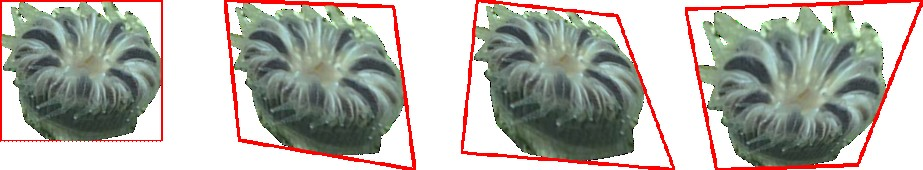
\includegraphics[width=140mm]{figs/implementation/ct/perspect.jpg}
    \caption{Various examples of the \textbf{Perspective transform}}
    \label{fig:ct_flip}
\end{figure}
\noindent This transform aims to emulate the effect of seeing a creature from different camera angles. To create this effect, I randomly move the four corners of creature, then transform the original image into the new quadrilateral using OpenCV's \verb|warpPerspective| function.

\subsubsection{Distortion}
\begin{figure}[h]
    \centering
    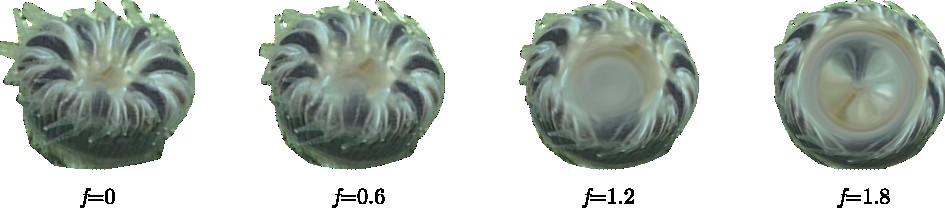
\includegraphics[width=140mm]{figs/implementation/ct/distort.jpg}
    \caption{\textbf{Distortion transform} controlled by factor $f$}
    \label{fig:ct_flip}
\end{figure}
\noindent This transform aims to emulate the way a soft body expands and retracts. Based on an algorithm for correcting lens distortion, this method first identifies a random pixel on a creature, the morph the regions around it to be larger or smaller than the original image. 

I chose to not include any transformations that affect the colours of the creatures as I believe these transforms are better suited when applied to entire images, rather than on an isolated image.

\subsubsection{Transformation pipeline}
All the transformations described are probabilistic. The parameters of transformations are randomly sampled at run time. Each transformation contains attributes that describe the probability distribution of the parameters. Multiple transforms can be stacked into an sequential pipeline. With the help of Dr Emily Mitchell, I created transformation pipelines suitable to each class of creatures. These custom pipelines were stored in `JSON' files and were loaded at run time to create  transformation pipelines.


\subsection{Creature Location Generation}
The next step was to find locations in existing images where the new creatures may be added. There are two possible methods of incorporating a new creature into an existing image. 

\subsubsection{Pasting}
In each image, the pasting algorithm first finds regions where a new creature could be placed. We shall call these regions \textit{proposal boxes}. The proposal boxes are generated through trial and error, where each newly generated proposal box must not overlap with any existing bounding boxes. The aspect ratios (ratio between height and width) the relative sizes of the proposal boxes were randomly sampled from actual bounding boxes from the data.

It is generally not advisable to paste new creatures near the top of images, as this is usually water body above the sea floor. Therefore, an additional empirical rule filters out all proposal boxes that are too far above the location of actual organisms in the image.

\subsubsection{Replacement}
The replacement algorithm first removes an existing creature from the image. Image inpainting techniques are applied to hide the empty space left behind by the removed creature. After experimenting with various options, I settled on the inpainting technique proposed by Telea \cite{telea_image_2004}, part of the \verb|OpenCV| library. The major drawback of inpainting is the high computation cost and inevitable visual artefacts. Thus, I found it generally not ideal to apply replacement on large sections of an image.

\subsubsection{Trade-offs}
Pasting offers greater efficiency at the risk of adding creatures to unsuitable locations. Replacement will always place creatures at suitable locations, but is computationally more expensive and does not scale well to large creatures. With these in mind, I decided to use both techniques simultaneously, preferring pasting for larger creatures and replacement for smaller creatures.

\subsection{Matching}
After pasting and replacing, I have a set of potential locations where new creatures could be added and a set of cropped creatures that can be added. The next step is to assign each potential location a suitable cropped creature. 

There are many factors to consider in this process.
\begin{itemize}
    \item \textbf{Pixel dimensions}. It is undesirable to stretch a low resolution cropped creature over a large area. It may be more acceptable to shrink a higher resolution cropped creature to fit into a smaller space.
    \item \textbf{Aspect ratio}. A similar aspect ratio is needed to prevent excessive stretching.
    \item \textbf{Relative size in image}: This measures how much of an image does a creature/space occupy. 
\end{itemize}

This was the most difficult part of this generation algorithm. I experimented with different ways to weight these factors, generating batches of a hundred example for each candidate method and manually inspecting them for the quality of matching. The final method weights aspect ratio most heavily, followed by relative size in image and pixel dimensions. 

\subsection{Extension: Creature Generation using GAN}
In this section, I detail how I completed an extension for this project, which is to generate new creatures using a Generative Adversarial Network (GAN). GAN is a type of deep learning model that consists of two neural networks, a generator and a discriminator. The two models are trained simultaneously to produce high-quality synthetic data. The generator network generates synthetic data samples while the discriminator network distinguishes between real and fake data. Thus, the objectives of the two models are adversarial in nature and the quality of the generated improves as a result of this competition.

As I have no prior experience with GAN, I wanted to use a GAN architecture that has the maximises the chance of successfully training. After some research, I found that InfoMax-GAN \cite{lee_infomax-gan_2020}, proposed in 2020 by a fellow Cambridge CST alumni, best fitted my requirements. By maximising mutual information between input data and its learned representation, InfoMax-GAN mitigates the risk of catastrophic forgetting and mode collapse, both of which are common training failures that I know I will struggle to resolve.


I trained the GAN models using manually extracted creatures. To increase the variance in input data, I applied random creature transforms. Figure \ref{Fig:gan_gallary} showcases a model trained for over 20000 training steps on examples of stony corals.

\begin{figure}[H]
\begin{tabular}{ll}
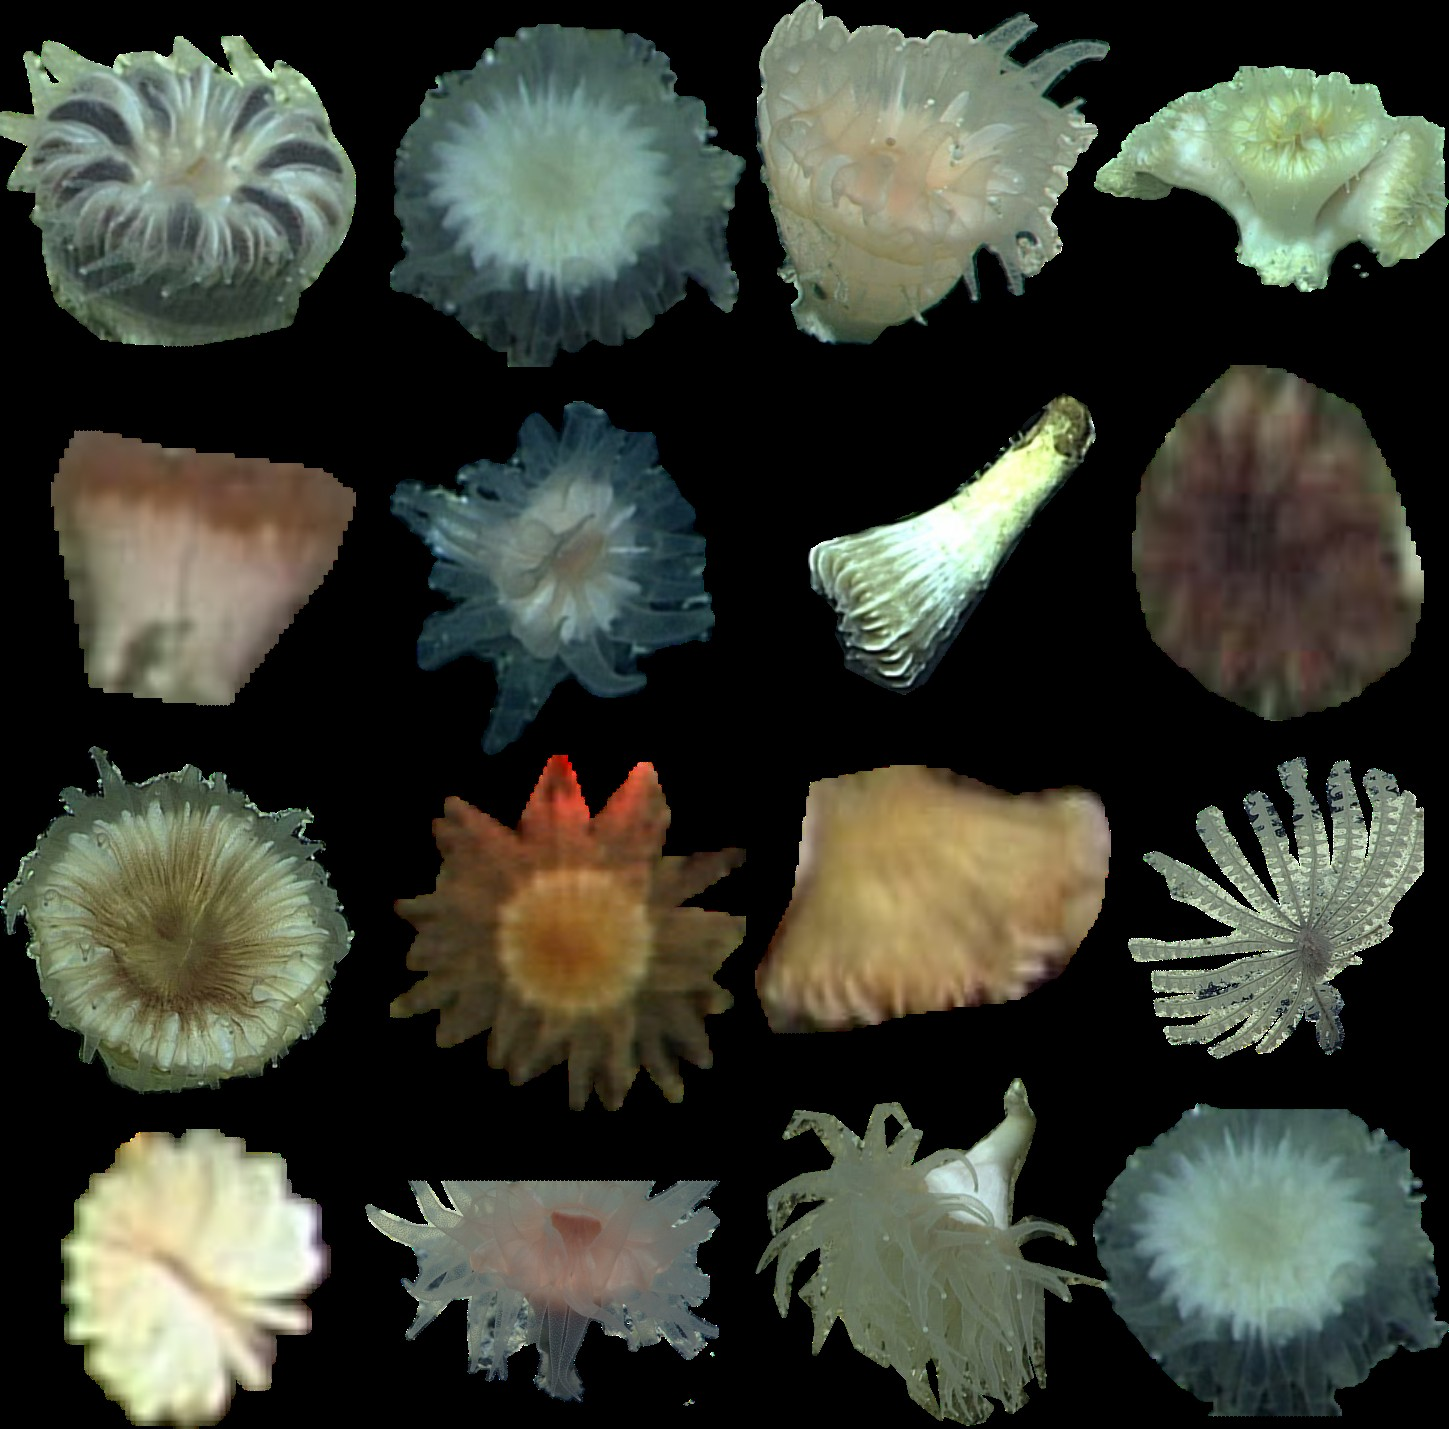
\includegraphics[width=0.47\textwidth]{figs/implementation/gan/actual.jpg} &
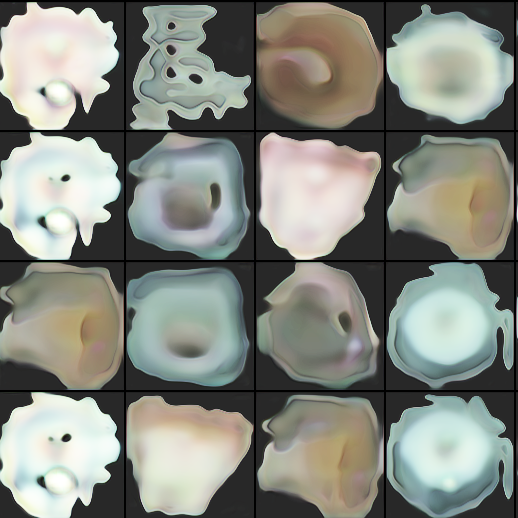
\includegraphics[width=0.47\textwidth]{figs/implementation/gan/generated.png}
\end{tabular}
\caption{\textbf{Demonstration of GAN generation: Left. Randomly selected training examples of stony corals. Right. Result of InfoMax-GAN generation.} The generated output mimics the training data at a glance, but is missing much of the fine-grained details. }
\label{Fig:gan_gallary}
\end{figure}

Despite the considerable amount of training, the output of the model did not capture the fine-grained details of the training example. I can attribute this to the following reasons:
\begin{itemize}
    \item Despite the aggressive creature transforms I have applied, the training data is small, consisting of just over 100 images. The discriminator network could have memorised the real images, making it very difficult for the generator to fool it. This is consistent with the training loss observed as the discriminator loss was consistently lower than the generator loss for most the training.
    \item The generated image was limited to $128 \times 128$ pixels, which is insufficient for the emergence of fine details.
\end{itemize}

I decided not to include the generated images into the main dataset.


\subsection{New Class Breakdown} \label{section:new_class}
After completing the training example generator, I used it to generate training examples for the three classes with the fewest number of training examples: ``black corals'', ``stony corals'' and ``demosponges''. Table \ref{table:new_classes} provides a new class breakdown after the generated images have been added to the dataset.
\begin{table}[H]
    \centering
    \begin{tabular}{| c c c r |}
        \hline
         \textbf{Class} & \textbf{Before Generation}  & \textbf{After Generation} & \textbf{Change} \\
         \hline
         \hline 
        \textbf{Black corals}	& \textbf{145}	    & \textbf{4293}	& \textbf{+4148}\\
        \textbf{Stony corals}	& \textbf{105}	    & \textbf{7950}	& \textbf{+7845}\\
        \textbf{Demosponges}	    & \textbf{963}	    & \textbf{6260}	& \textbf{+5297}\\
        Glass sponges	& 2907	& 3544	& +637\\
        Sea pens	    & 3008	& 4308	& +1300\\
        Sea cucumbers	& 6075	& 7250	& +1175\\
        Starfish	    & 6778	& 7962	& +1184\\
        Sea anemones 	& 7580	& 9629	& +2049\\
        Soft corals	    & 7991	& 9144	& +1153\\
        Sea pigs	    & 8348	& 9152	& +804\\
        Sea urchins	    & 13234	& 17070	& +3836\\
        \hline
         \hline
         \textit{Total} & 57134 &  86562 & +29428\\
         \hline
    \end{tabular}
    \caption{\textbf{Breakdown of annotations in the dataset, before and after example generation.} Note that the newly generated images could include annotations of other classes, creating new annotations for all classes.}    
    \label{table:new_classes}
\end{table}

With the training example generator, the ratio of example counts between the smallest and the biggest classes decreased from over 100 to less than 5. For the rest of the project, the newly generated examples will be used for training and not testing.

\subsection{Gallery}

Figure \ref{Fig:exgen_gallary} showcases example outputs from the training example generator.

\begin{figure}[h!]
\begin{tabular}{ll}
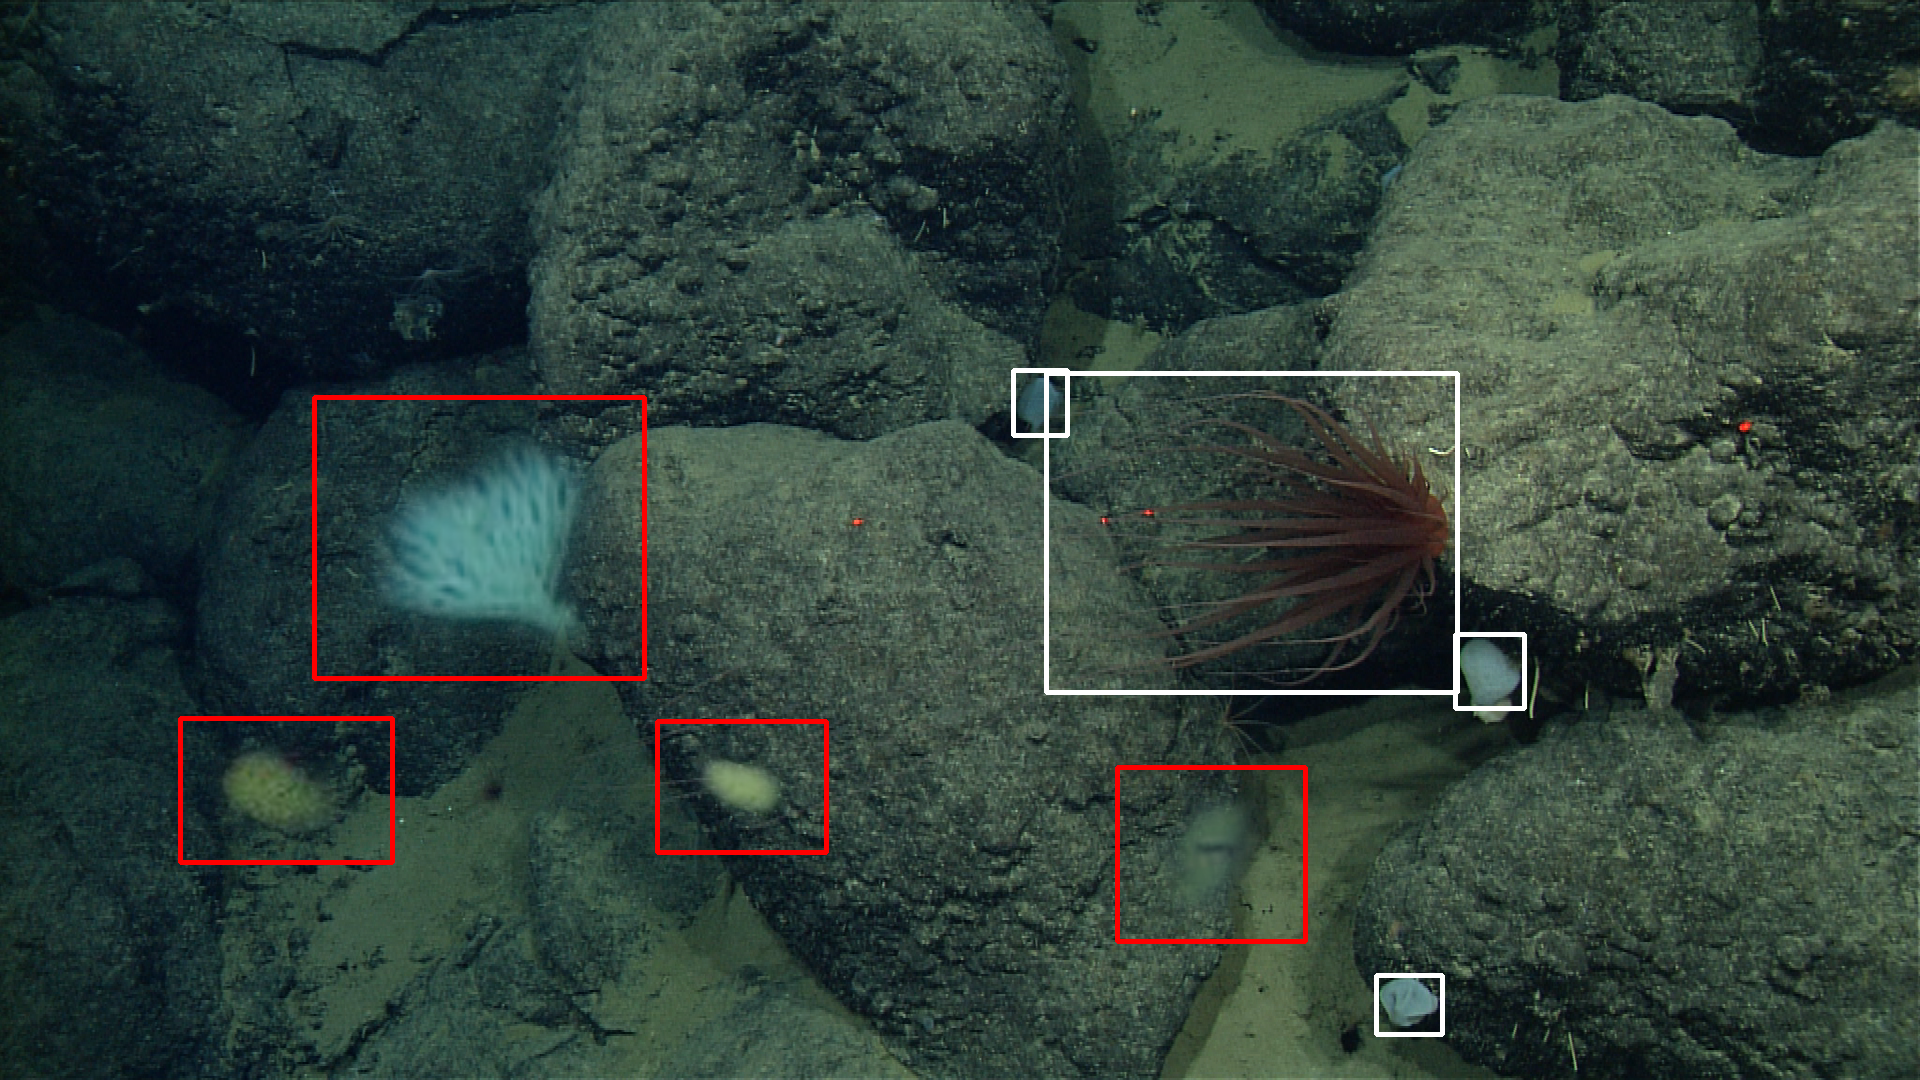
\includegraphics[width=0.5\textwidth]{figs/implementation/exgen/1.png}&
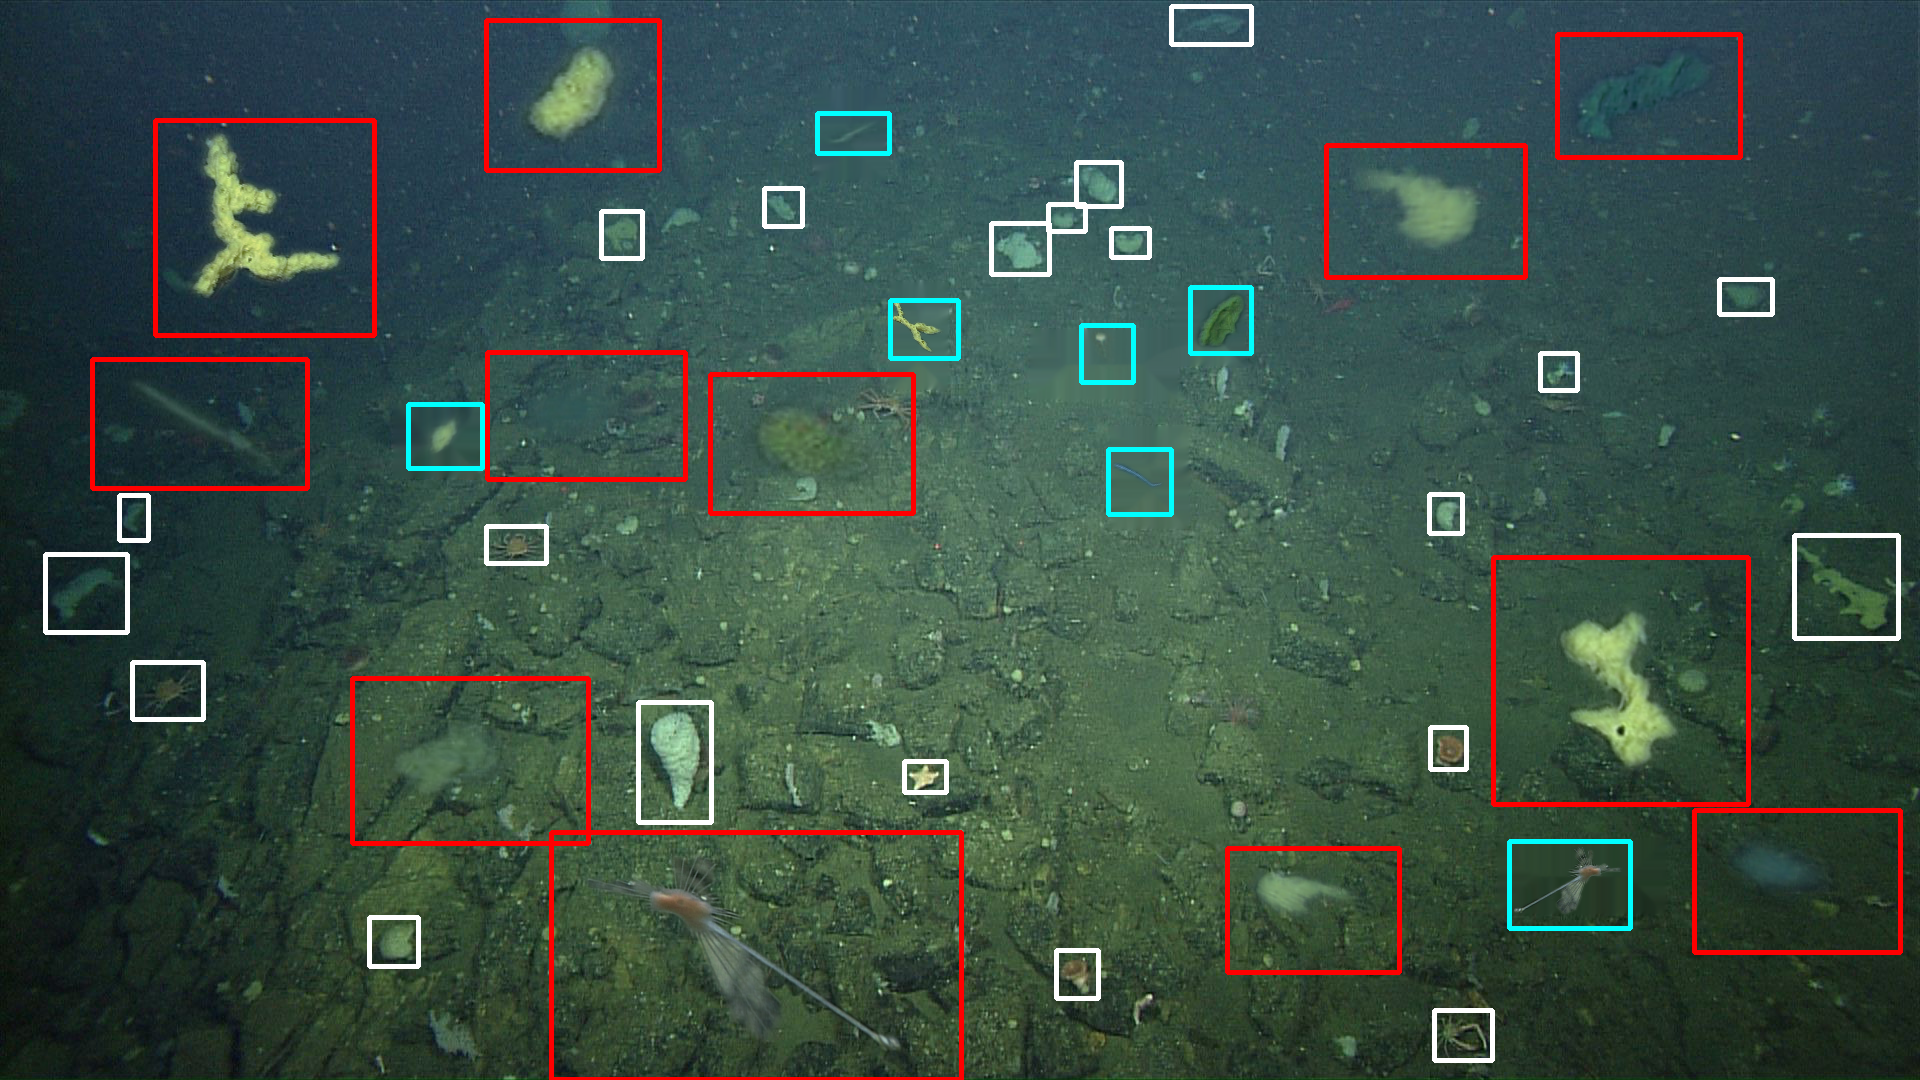
\includegraphics[width=0.5\textwidth]{figs/implementation/exgen/2.png}
\end{tabular}
\caption{\textbf{Example outputs of the training example generator.} Red and blue boxes indicate examples added by pasting and replacement respectively. White boxes indicates unmodified examples.}
\label{Fig:exgen_gallary}
\end{figure}


\newpage
\section{EfficientDet}
EfficientDet \cite{tan_efficientdet_2020} is a one-stage object detection model published in 2020. It is based on EfficientNet \cite{tan_efficientnet_2020-1}, an image classification model published in 2019. 
A major feature of EfficientDet is \textit{compound scaling}, where a single integer hyperparameter adjusts all dimensions of the model and produces different variants of EfficientDet that caters to different performance and efficiency requirements. The many variants of EfficientDet would allow greater room for experiments

\subsection{Architecture}
In this section, I will cover the major components of EfficientDet and explain how it is used for detection and classification.

\begin{figure}[h]
    \centering
    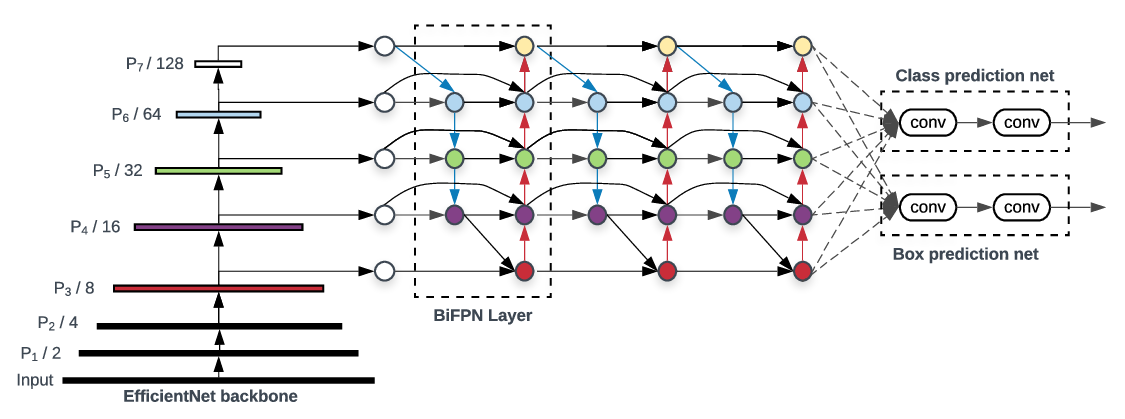
\includegraphics[width=0.9\textwidth]{figs/implementation/efficientdetarch.png}
    \caption{EfficientDet architecture. \cite{tan_efficientdet_2020}.}
    \label{fig:efficientdetarch}
\end{figure}

\subsubsection{EfficientNet backbone}
EfficientDet uses EfficientNet \cite{tan_efficientnet_2020} as its backbone. An input image is first forward propagated through EfficientNet, then outputs at selected convolutional layers are extracted and stacked. As each of extracted layer has a different resolution, we refer to this stack of features as the \textit{feature pyramid}. 

\subsubsection{BiFPN}
Weighted Bi-directional Feature Pyramid Network (BiFPN) is a scale feature fusion network. The purpose of the network is to combine convolutional features from different resolutions so as to produce semantically more meaningful features. When combining features of different resolutions, BiFPN takes a weighted sum of input feature maps.
\begin{align}
    O=\sum_i \frac{w_i}{\epsilon + \sum_j w_j}\cdot I_i
\end{align}
Where $I_i$ are input features and $O$ is the output feature; $w_i$ are learned weights for each input feature map, and $\epsilon$ is used to ensure numerical stability.

\subsubsection{One-stage detection and classification}
The output of the final BiFPN layer was passed to two separate convolutional neural networks for detection (bounding box regression) and classification. As described in section \ref{section:one_stage}, each grid cell in the input image was associated with a fixed number of anchor boxes. EfficientDet uses a total of 9 anchor boxes of 3 different sizes and 3 different aspect ratios.  

\begin{figure}[h]
    \centering
    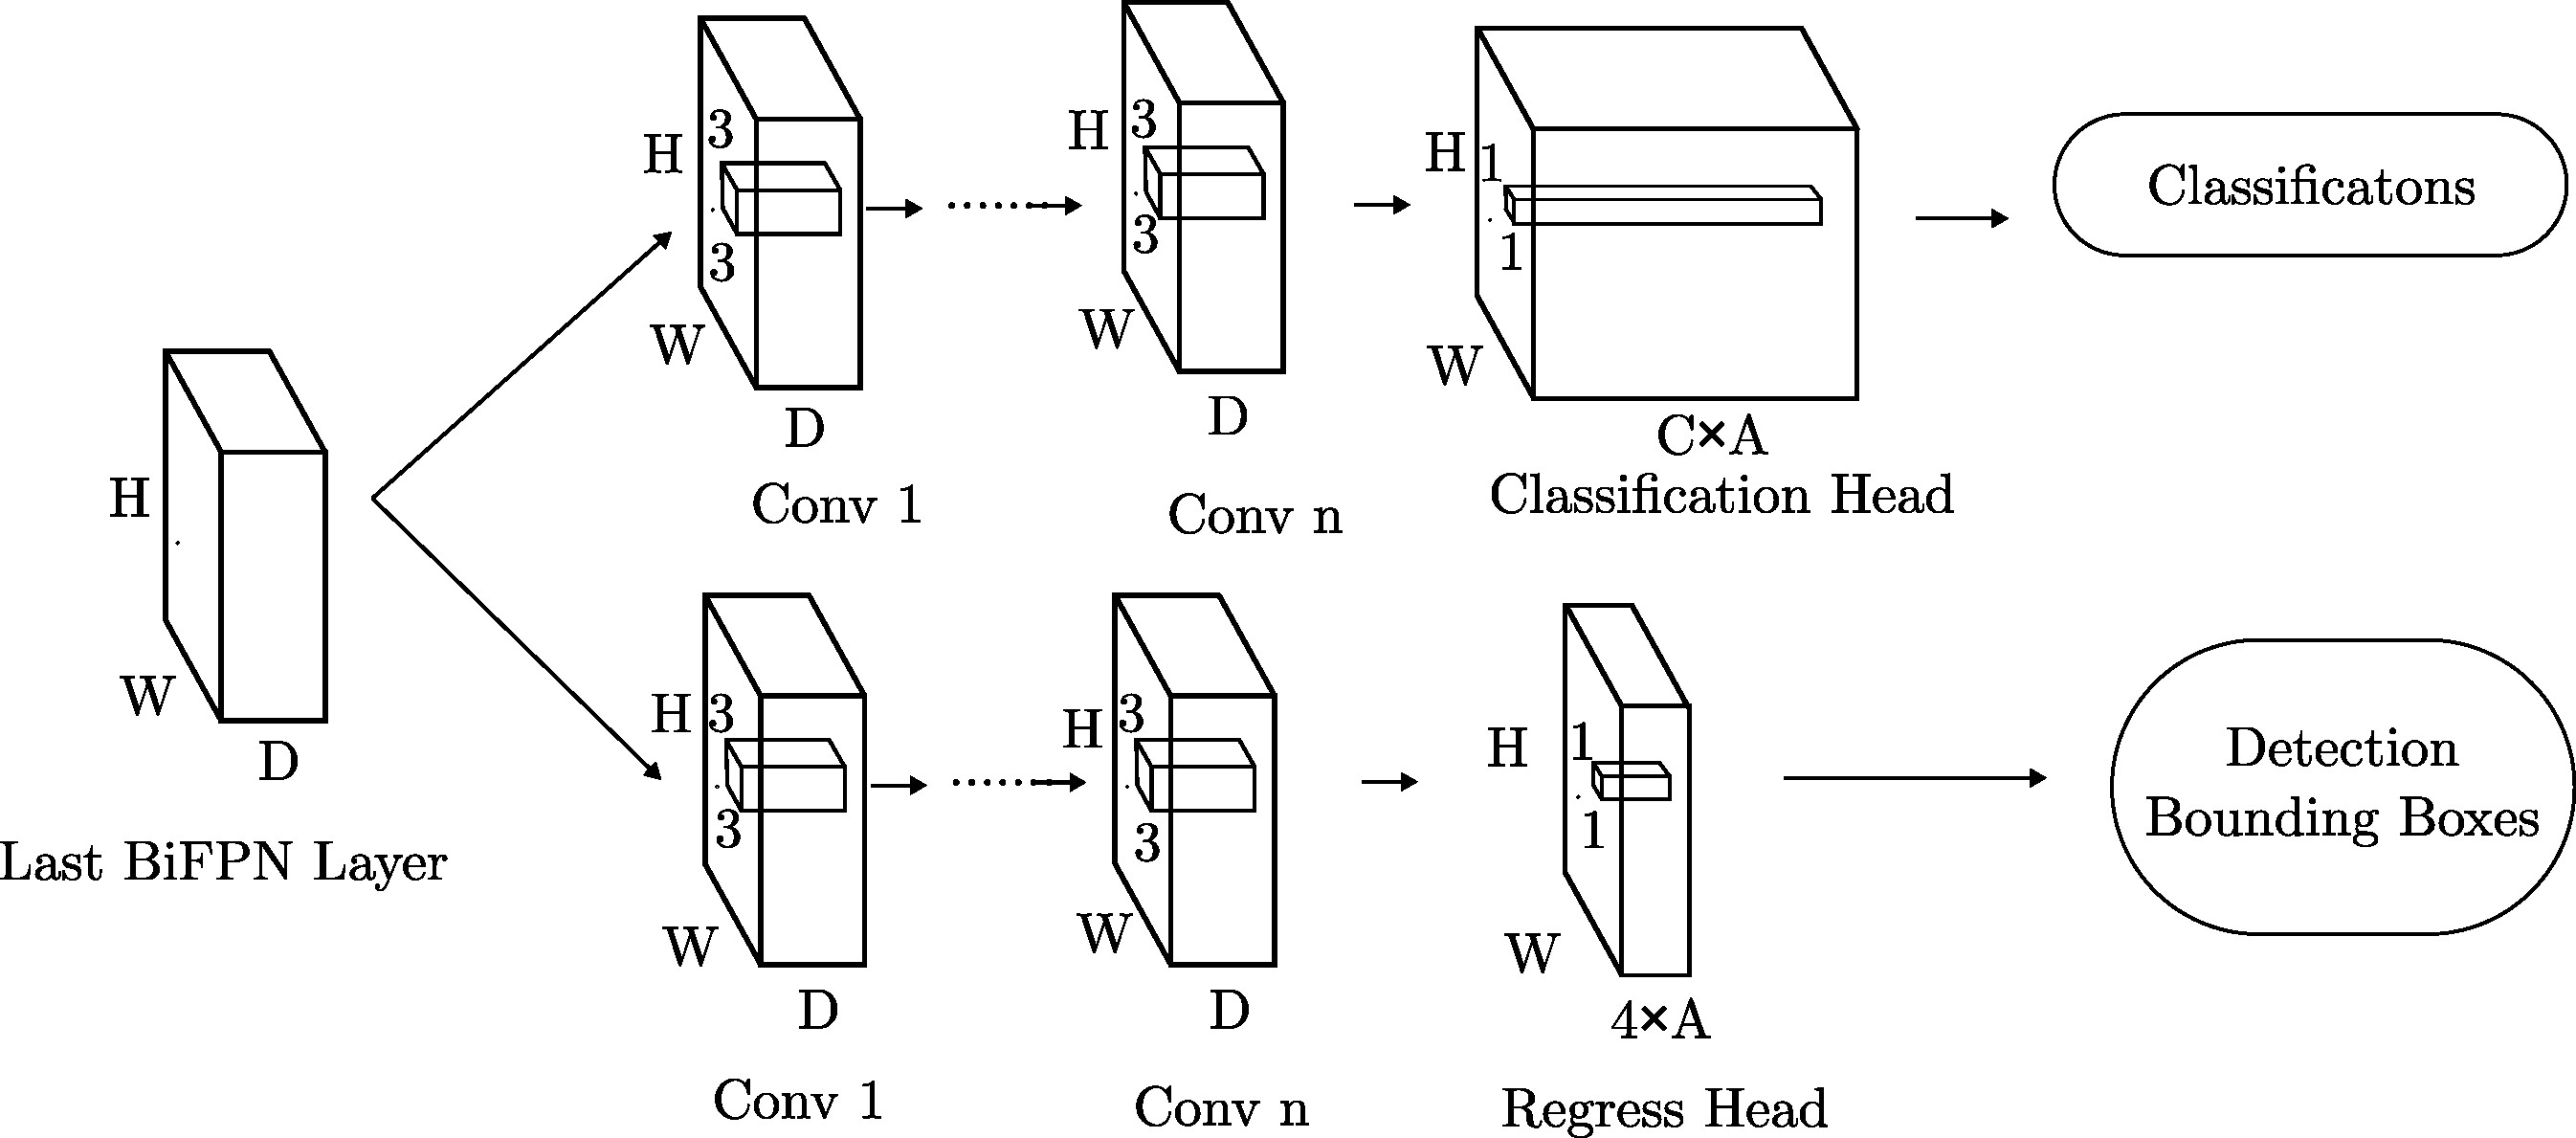
\includegraphics[width=0.9\textwidth]{figs/implementation/efficientdet_heads.jpg}
    \caption{\textbf{EfficientDet Detection and Classification Architecture}: The detection and classification modules branches off from BiFPN output.}
    \label{fig:edet_heads}
\end{figure}
\subsubsection{Box prediction net}
For every anchor box, the detection module is trained to predict 4 transform parameters that map the anchor box bounding boxes to the ground truth bounding boxes. 

\subsubsection{Class prediction net}
For every anchor box, the classification module is trained to predict a confidence score for every class. The sigmoid function ($S(x)=\frac{1}{1+e^{-x}}$) is applied on module output to map the output between 0 and 1. Note that softmax is not used here as the model is trained to represent ``No object detected'' by predicting a low confidence score for every class.

\subsection{Losses}
\subsubsection{Detection: Smooth L1 Loss}
For regression loss, EfficientDet uses Smooth L1 loss. For prediction $x$ and truth $y$, Smooth L1 loss is defined as: 
\begin{align} \label{eq:smooth_l1}
    \regloss = \begin{cases}
        \frac{1}{2\beta}(x-y)^2\quad\ \text{if } |x-y| < \beta\\
        |x-y|-\frac{1}{2\beta}\quad \text{otherwise}
    \end{cases}
\end{align}

\subsubsection{Classification: Focal Loss}
For classification loss, EfficientDet uses Focal Loss \cite{lin_focal_2018} proposed in 2017. Focal Loss downweighs the contribution of easy examples on the total classification loss. This helps to focus training on difficult examples. Focal loss is controlled by the parameter $\gamma$. The greater the value of $\gamma$, the greater the skew introduced by focal loss. If $p$ is the model's estimated probability and $y$ is the label, focal loss is defined as:


\begin{align}\label{eq:focal}
p_t&=\begin{cases}
    p\quad\quad\text{if }y=1\\
    1-p\ \text{otherwise}
    \end{cases}\\
\clsloss &= -(1-p_t)^\gamma \log(p_t)
\end{align}
When $\gamma=0$, the focal loss becomes $-\log(p_t)$, which is equivalent to cross-entropy loss.

\subsubsection{Total loss}
Combining the detection and classification losses, we derived a formula for the total loss of EfficientDet:
$$
\mathcal{L}^{\text{total}} = \clsloss + \kappa\regloss
$$
 Where $\kappa$ is a tuned hyperparameter. 

\subsection{Implementation}
I implemented both EfficientNet and EfficientDet from scratch. Before starting, I read both research papers and created notes about their respective architectures. For details not covered in the research papers, I consulted the official implementations of the models, both of which was for TensorFlow. I sketched the architecture of both models on my iPad and annotated it with the details I have collected from my research. As this was my first time implementing a model in PyTorch, I followed PyTorch tutorials on writing custom CNN models and researched on the best practises when writing PyTorch modules.

An interesting challenge which emerged from this process was subtle differences between TensorFlow and PyTorch. For example, The official implementation of EfficientNet used a feature of TensorFlow's convolutional layer which was unavailable on PyTorch. If unresolved, my EfficientNet implementation would produce different output dimensions to the original implementation, thus invalidating it. To key to solving this lies on applying to a custom padding to PyTorch input data. Through repreated experiments with different input sizes, I worked out a solution and wrote a test to ensure my approach consistently behaves the same as its counterpart in TensorFlow. 

Another issue I learnt to be mindful of is numeric instability, which affected my implementation of Focal Loss (Equation \ref{eq:focal}). I learned to be careful with $\log$ functions and divisions when the input could be close to zero. I was able to resolved the numeric instability issues by clipping input to within a safe range.


\section{Supervised Contrastive Learning}
In this section, I detail my implementation of supervised contrastive loss \cite{khosla_supervised_2021} for marine creature classification. As there is very little published work on applying supervised contrastive learning for object detection, this part of the project required significant trial-and-error and was one the most time consuming part of this project.

\subsection{Motivations}
In terms of physical features, creatures grouped by taxonomic classes are marked by high intra-class differences and high inter-class similarities. This is because taxonomic classes group together genetically-similar organisms, but genetically similar organisms can have very different appearance. On the other hand, evolutionarily distant organisms may develop similar physical features when exposed to similar external stimuli. Thus, classifying creatures into taxonomic classes requires a model to spot subtle features that set different classes of creatures apart. 

\subsection{Problem Analysis}
The problem of porting supervised contrastive loss to EfficientDet boils down to two important questions:
\begin{enumerate}
    \item \textit{What are the object features?}\\ 
    Recall that supervised contrastive learning aims to maximise similarity between features of similar concepts while minimising the similarity between different concepts. In this context, concepts refer to the labelled objects in the images. To implement supervised contrastive loss, I need to derive features for every labelled object.

    EfficientDet provides `grid cell' features that correspond to different regions of the image. How do I transform these features into object features?
    \item \textit{How do I train with contrastive loss?}\\
    Supervised contrastive loss \cite{khosla_supervised_2021} is proposed for the one task of image classifications. Object detection requires training for both detection and classification tasks. How should I mix both tasks at training time?
\end{enumerate}

\subsection{First approach}
In my first attempt, I sought to closely emulate the supervised contrastive (SupCon) loss technique proposed by Khosla et al. \cite{khosla_supervised_2021}.

\subsubsection{SupCon Loss}
For a batch of examples with normalised features $\{\mathit{z}_1, \dots, \mathit{z}_n\}$ and labels $\{y_1, \dots, y_n\}$, supervised contrastive loss is defined as:
\begin{align}
    A(i) &= \{a \in [1,n]\ |\ a \neq i\}\\
    P(i) &= \{p \in A(i)\ |\ y_p = y_i\}\\
    \suploss &= \sum\limits_{i\in [1, n]}\suploss_i=\sum\limits_{i\in [1, n]}\frac{-1}{|P(i)|}
    \sum\limits_{p\in P(i)}\log\frac{\exp{(\mathit{z}_i \bullet \mathit{z}_p})}{\sum\limits_{a \in A(i)}\exp{(\mathit{z}_i \bullet \mathit{z}_a)}} \label{eq:supcon}   
\end{align}
In the equations, $\bullet$ represents the vector dot product. In SupCon loss, all input vectors are normalised, so $x \bullet y$ is equal to the cosine similarity between vectors $x$ and $y$. thus minimising $\suploss$ maximises cosine similarity between same-class embeddings and minimises the cosine similarity between different-class embeddings.

\subsubsection{Sources of positive and negative pairs} \label{section:scl_double}
In my implementation, there are two sources of positive pairs and two sources of negative pairs:
\textbf{Positive Pairs:}
\begin{enumerate}
    \item For each input image, an augmented version is generated through image augmentation techniques introduced in Section \ref{section: data_aug}. This guarantees at least one positive pairs for each creature. This technique doubles the training cost when supervised contrastive learning is used.
    \item Creatures from the same batches of the images that share the same class.
\end{enumerate}

\textbf{Negative Pairs:}
\begin{enumerate}
    \item Creatures from the same batches of the images that are of a different class.
    \item All creatures should be contrasted with the background. Thus, hard negative mining as done to create examples of the background.
\end{enumerate}

\subsubsection{Two stage training}
Khosla et al. \cite{khosla_supervised_2021} showed that SupCon loss could replace traditional supervised loss for image classification. They presented a two stage training technique. In the first stage, the image classification model is trained for over 700 epochs on the SupCon loss (Equation \ref{eq:supcon}) alone. In the second stage, the final classification layer of the model is trained for 10 epochs while the rest of the model parameters were frozen. 

Applying this training technique to object detection introduces the problem of when to do regression training. I decided to introduce an additional SupCon loss for regression that contrasts between background and foreground regions. Examples of background regions were generated by negative mining. Together, the training losses are described in \ref{eq:subcon_1}


\begin{align*} \label{eq:subcon_1}
    \textbf{Stage 1: }& \suploss_\text{cls} + \kappa_1\suploss_\text{reg}\\
    \textbf{Stage 2: }& \clsloss + \kappa_2 \regloss
\end{align*}

Here $\kappa_1$ and $\kappa_2$ are tuned hyperparameters. 
Note that the second-stage loss function is equivalent to the loss function of the unmodified EfficientDet. Thus, this training methodology essentially represents EfficientDet with contrastive pretraining.

\subsubsection{Object features from feature vectors} \ref{secion:old_creature_feature}
For one-stage detection models such as EfficientDet, there is no direct way to retrieve embeddings for particular regions of an image. Instead, the model produces feature vectors that encapsulate the information from pre-defined grid cells. I derived the feature representation of an object as the weighted sum of feature vectors of grid cells that overlap with the object. The weight depended on the extent of overlap between the creature and the anchor box, as well as the distance between the centre of the creature and the anchor point. 


\subsubsection{Projection network}
Instead of using EfficientDet activations directly as input to SupCon loss, I first transformed the activations using a multilayer perceptron (MLP) with one hidden layer. This non-linearity is called the \textit{projection head} and has been demonstrated to improve the quality of learnt representation \cite{chen_simple_2020}. The projection head is only used for contrastive loss calculation and is discarded after training. The dimensionality of the projected space, $\mathcal{D}^p$, is a tuned hyperparameter. 


\subsection{Problems}
I had to abandon the approach as described above due to a lack of training time. When training, I observed a very slow convergence in supervised contrastive loss. 
In Khosla et al. \cite{khosla_supervised_2021}, supervised contrastive pretraining required 700 epochs on the batch size of at least 256.
One epoch of training using Efficient-D2 takes approximately 0.8 GPU hours on the Cambridge HPC. This means completing 700 epochs would take approximately 560 GPU hours, representing a significant proportion of the total 3,000 GPU hours allocated to the project just for a single set of training. Moreover, hyperparameter tuning could require multiple round of training, easily using up all available GPU hours. In fact, the heavy utilisation of the HPC meant that it was impractical to expect that amount of training time. In the interest of risk mitigation, I decided that it was prudent to abandon the technique.

\subsection{Reflection}
While supervised contrastive pretraining proved difficult, the SupCon loss could still be useful when used together with supervised losses. A similar technique was applied in Tanveer et al. \cite{tanveer_regularization_2021} which experimented with using contrastive losses as regularization for image classification. Their results showed accuracy improvements of 1.24\% in the CIFAR-10 dataset and 11.46\% in the CIFAR-100 dataset \cite{noauthor_cifar-10_nodate}, with contrastive regularization reducing inter-class confusion. 

\subsection{Second Attempt} \label{section: final supcon loss}
\subsubsection{One stage training}
A new one-stage training methodology with loss function will be used:
$$
\clsloss + \kappa_1 \regloss + \kappa_2 \suploss
$$
$\kappa_1$ and $\kappa_2$ are tuned hyperparameters.

\subsubsection{Dynamically adjusted object feature}
In my previous implementation of the SupCon loss, I calculated object features by collecting the grid cells that overlap with the object and taking a weighted sum of their feature vector. As grid cells are predefined and constant, there was a constant mapping between object feature and convolutional output. This was sufficient for the previous approach, where bounding box regression was trained after supervised contrastive learning. With the new approach, the model is trained on bounding box regression as well, which means that anchor boxes of the model changes constantly during training. The constant mapping as proposed before could not adapt to this change. This leaves potential for a more granular approach, which takes weighted sums over changing anchor boxes instead of static grid cells.

\begin{figure}[H]
    \centering
    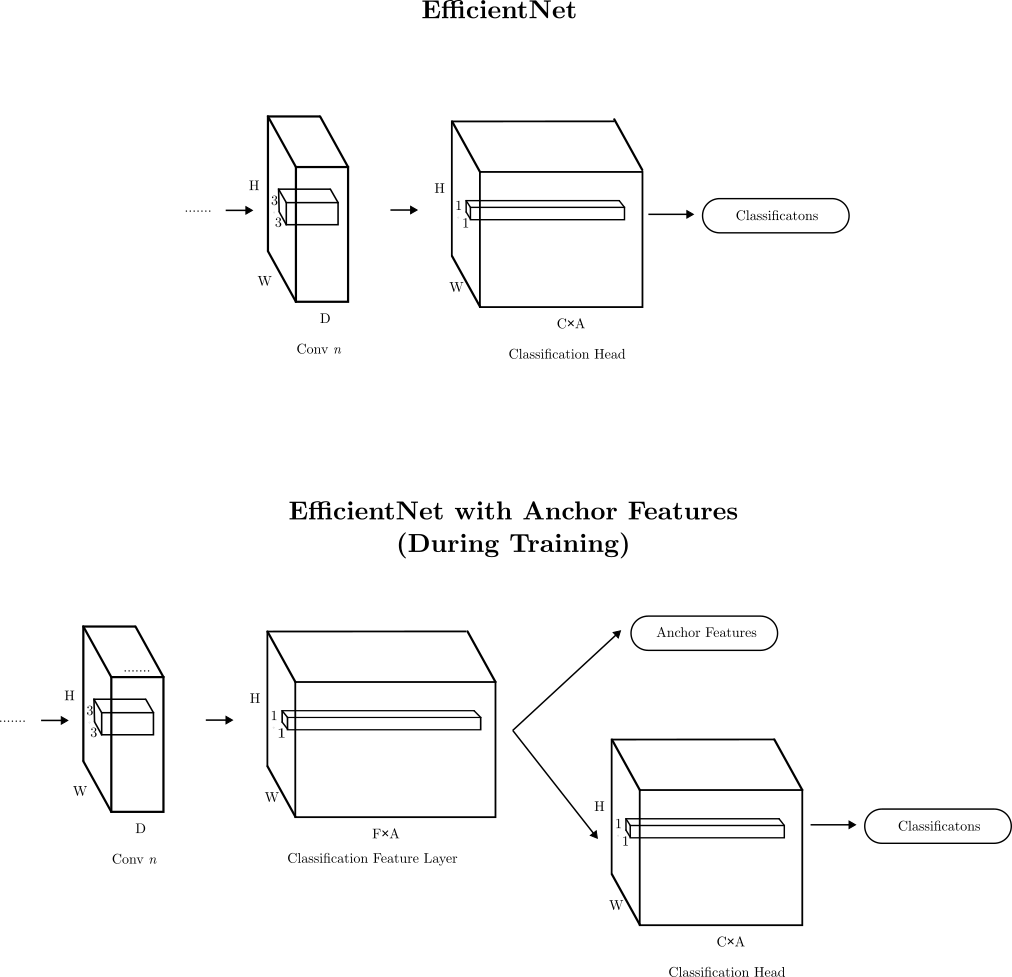
\includegraphics[width=0.8\textwidth]{figs/implementation/efficientdet_new_head.png}
    \caption{\textbf{Before and after splitting the final layer for anchor features.} \texttt{A} is the number of anchors per grid cell. \texttt{C} is the number of classes. \texttt{F} is the vector length of anchor features. \texttt{H},\texttt{W} and \texttt{D} are the dimension of convolutional output.}
    \label{fig:edet_new_head}
\end{figure}

However, before designing such a technique, I was contended with the problem that there existed no feature representation for anchors. As explained in section \ref{section:one_stage}, one-stage object detector output feature vectors for each grid cell, each grid cell in turns is associated with multiple anchors. How would one break one feature vector into anchor vectors? I decided to separate the final linear layer (as a form of a $1\times1$ convolutional layer) into two linear layers. The first layer learns to produce anchor features from a grid cell feature. The second layer learns to map anchor features into desired model output. Figure \ref{fig:edet_new_head} illustrates the effect of applying this technique to the final layer of the EfficientDet classifier.

During training, this technique required a modification to EfficientDet's model architecture. After training, the two linear layers can be collapsed into one. In my implementation, I defined the class \verb|EfficientDetPerAnchor| for the training model and defined a function that converts it to the standard EfficientDet class \verb|EfficientDet|. 

Putting the pieces together, my new approach calculates the latest anchor boxes during forward propagation. It then calculates the Intersection-over-Union (IoU) (defined in section \ref{section:explain_miou}) between every object and anchor box. For each object, the top-$k$ anchor boxes were selected and the weighted sum of their feature vector was taken as the object feature. I calculate the weight for each anchor box by the inverse power law where the weightage of the $i$-th anchor box is $\frac{1}{i^{\gamma}}$, where $\gamma$ is a tuned hyperparameter.


\section{Training and Hyperparameter Tuning}
Given the size of the dataset and the memory and compute requirement of model training, it was impractical to train the models for this project on my own computer. This project is completely trained on the Cambridge High Performance Computing (HPC) cluster.

\subsection{Training on the Cambridge HPC Cluster}
Cambridge HPC was the first centralised computing facility that I have used, so it took me some trial and error to get used to submitting jobs with the \verb|slurm| system. The Cambridge HPC documentation proved very useful, and I gained confidence in the system by submitting successively larger jobs. For each submitted job, I directed its outputs to \verb|~/outputs/<job_id>.out|. In the preamble of each job, I included bash commands that outputs the state of the machine and the kernel modules loaded, as this proved helpful for debugging. To interact with the HPC servers, I used \verb|ssh| and with SSH tunnelling, I was able to access graphical tools such as Jupyter Notebook and TensorBoard.

\subsection{Distributed Training}
I knew that distributed training would be required for the project from the beginning due to the large size of the dataset. Furthermore, the application of supervised contrastive learning (section \ref{section:scl_double}), as well as the dynamical generation of new training examples (section \ref{section:new_class}) both  increased the effective training required for this project. In total, both techniques roughly tribled the time required for one epoch of training. 

\subsubsection{Architecture}
The distributed training setup consists of many processes that can span multiple machines. Processes communicate with each other through the HPC Ethernet network and each has exclusive access to a GPU. One of the process is assigned as the primary process. The primary process took charge of I/O actions such as saving checkpoints, logging and passing values to other processes. 

For distributed model optimisation, I used the Pytorch component \verb|DistributedDataParallel| which produced a set up in which each process was given a disjoint subset of the training dataset. For each batch of training data, each process executes forward and backward propagation independently, then synchronise their gradients, and execute the same optimisation step. While \verb|DistributedDataParallel| handles this aspect of training, I achieved more nuanced control using the \verb|torch.distributed| utility which allowed to design custom inter-process communication. I enabled the nodes to ``vote'' to terminate training early and to alert all other nodes if they encounter training abnormalities (such as infinite or invalid gradient). Nodes also synchronised values such as validation loss and evaluation metrics to ensure every process has a consistent picture of the training progress. 

 I tested my setup on up to 8 GPUs. but observed diminishing return after more than 4 GPUs are used. This is likely due to a combination of increased cost of communication and the limits of paralellism as described by Amdahl's Law \cite{amdahl_validity_1967}. For most the project, I used distributed training over 4 GPUs. 

\subsection{Hyperparameter Tuning}
Performance of machine learning algorithms is critically dependent on identifying a good set of hyperparameters. A poor choice of hyperparameters could cause an otherwise well-designed model to perform poorly. Therefore, ample amount of hyperparameter tuning is important for fair evaluation.

\subsubsection{Tree-structured Parzen Estimator}
In this project, EfficientDet introduces 5 hyperparameters while various experiments with supervised contrastive loss introduced many more. The large size of the hyperparameter search space and very limited server time meant that I needed an algorithm that can efficiently sample a high-dimensional space.
Tree-structured Parzen Estimator (TPE) \cite{bergstra_algorithms_2011} is a Bayesian optimisation algorithm that models the search space using Parzen Estimation. Unlike random search or grid search, TPE updates its understanding of the search space after every sample, allowing faster convergence to good parameters.

\subsubsection{Hyperband Pruning}
When tuning hyperparameters, it is often desirable to terminate unpromising experiments early to conserve computational resources. However, this comes at the risk of removing good experiments that has yet to emerge. There is a trade-off between the decision to prune and to not prune. Hyperband \cite{li_hyperband_2018} is a technique that models this trade-off as a multi-arm bandit problem. I chose as it has been shown to produce good results.

\subsubsection{Setup}
I chose to use the \verb|optuna| library for hyperparameter as it provides both TPE and Hyperband pruning while offering excellent documentation. 
Hyperparameter tuning jobs were scheduled on the Cambridge HPC, and all the results were centrally collected and stored in a SQLite database. 
As I was only allowed jobs of up to 12 hours on the Cambridge HPC, I faced the problem of frequent premature termination of tuning trials. To overcome this, I implemented a resume system. During training, the hyperparameter tuning code automatically detects when it was about to be terminated. It then dumps all of the data into a temporary directory and writes the directory to a pre-defined file. Then, when another task is allocated server time, it starts by checking the predefined file and resumes from where the last trial ended if an entry was found. Special care was taken to ensure that there is no conflict with multiple jobs checking the file at the same time (even though this is very unlikely). Implementing this system required me to work around many restrictions imposed by the \verb|optuna| library. Careful reading of the library source code was needed to ``trick'' it into thinking two trials were the same. With this resume mechanism, tuning was able to proceed efficiently.

\subsection{Universal Training Architecture}
When experimenting with different training setups for supervised contrastive learning, I found myself repeatedly writing similar code for model training. This lowered productivity due from rewriting the same code and increased the chance of bugs from careless copying and pasting. This was especially undesirable as training and hyperparameter tuning was the time consuming aspect of this project. Bugs in training code could cause failures to train or invalidate trained model. To mintage these risks and to maximise code reuse, I designed an standard training architecture that was used to train all models in the project.

\subsubsection{Design}
\begin{figure}[H]
    \centering
    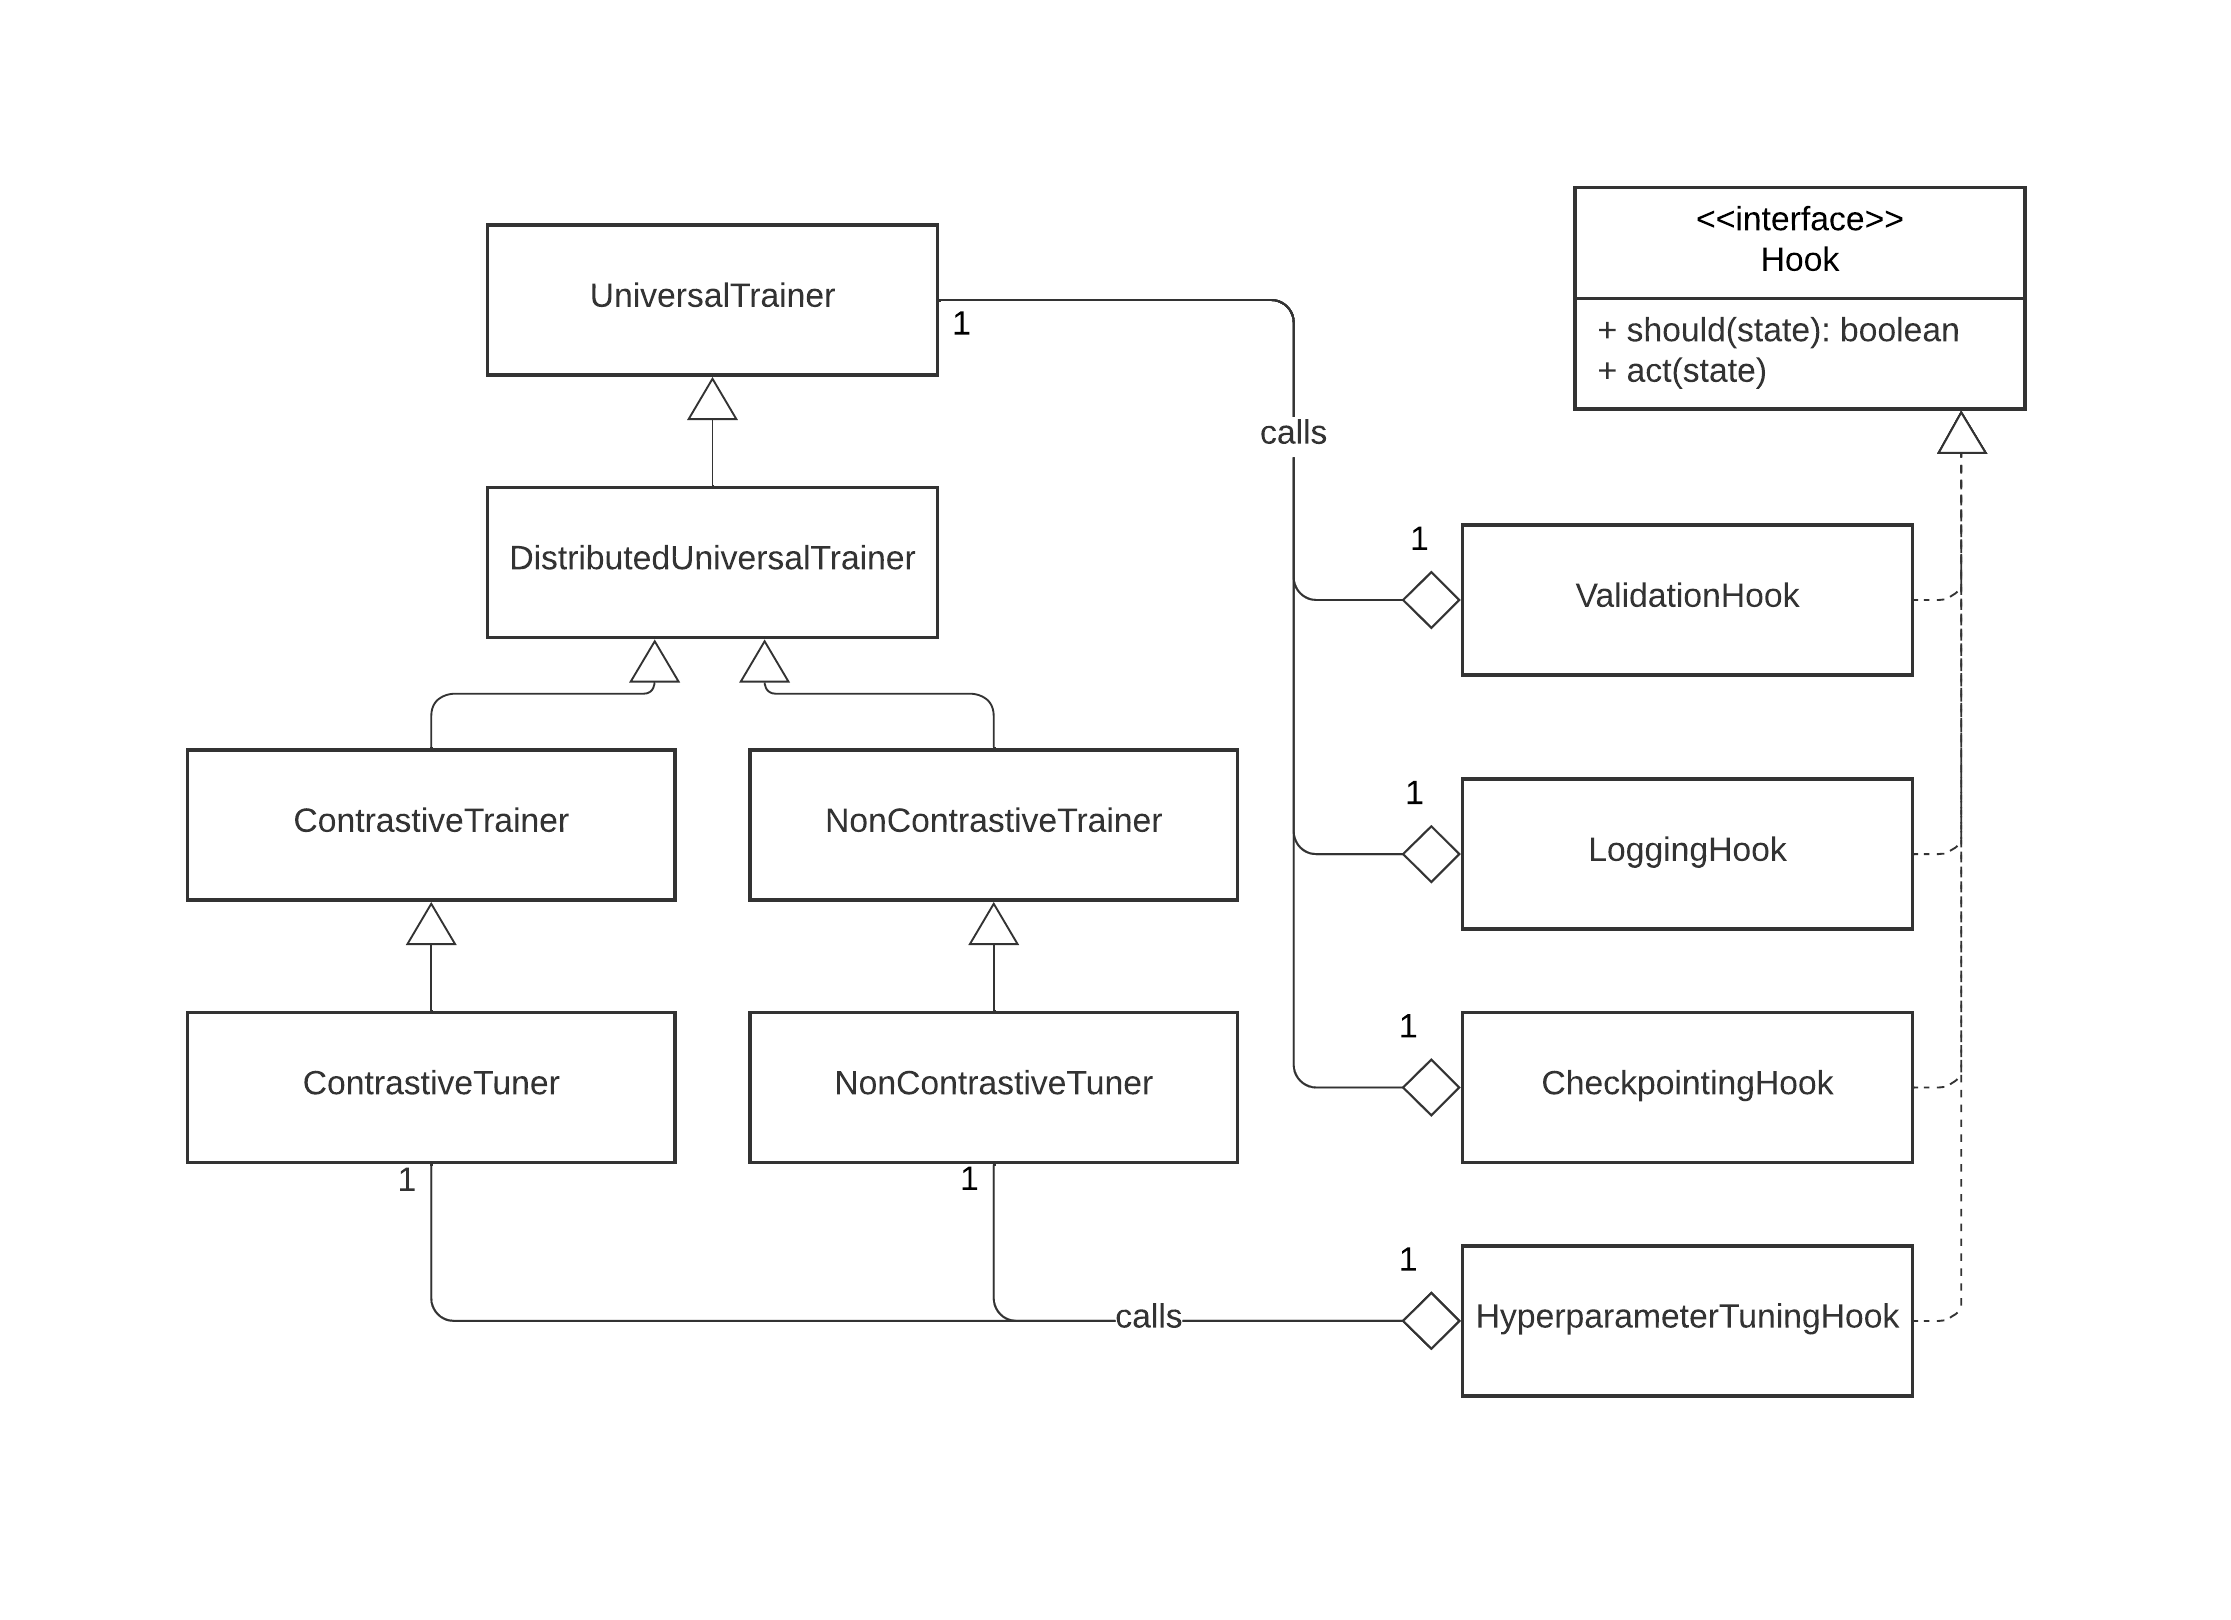
\includegraphics[width=0.7\textwidth]{figs/implementation/trainer/simple_uml.png}
    \caption{\textbf{A simplified UML diagram of the universal training architecture.}}
    \label{fig:simple_uml}
\end{figure}

The idea is to create a general architecture which follows the open–closed principle of object oriented programming. Figure \ref{fig:simple_uml} shows a simplified structure of the architecture.

The design maximises code reuse through inheritance. The base class \verb|UniversalTrainer| defines methods useful for all model training. I broke the typical model training loop into its major components, and implemented each component as a method of \verb|UniversalTrainer|. This way, a derived class can easily modify training behaviour by overriding a one of these method. 
\verb|DistributedUniversalTrainer| modifies some functions of \verb|UniversalTrainer| to ensure correct behaviour in a distributed training setup. It also contains useful functions such as value synchronisation. It is hard to debug and test distributed training code, thus unifying all relevant code in a single class was extremely useful. From \verb|DistributedUniversalTrainer|, various classes were defined for training with and without supervised contrastive loss.

To further enable code reuse, I designed the \textit{hook} system . A hook can encapsulate any code that is repeatedly executed during model training. This includes validation, logging and saving checkpoints to disk. Hooks are meant to be registered to a model. Once registered , the model calls the hook after every step or after every epoch of training. This system prevents having to rewrite common operations for every training loop. Hooks may be registered and deleted at run time, allowing for dynamic adjustment of training behaviour.

The flexibility of this system is demonstrated in its ability to support hyperparameter tuning. Each hyperparameter tuning class simply inherits from the normal training class and adds an additional hyperparameter tuning hook. This new hook is responsible for communication with the database and could trigger an early termination if needed. 

Instead of rewriting this code for every training loop, 


\verb|Distr|


\chapter{Evaluation}

In this chapter, I apply quantitative evaluation and qualitative analysis of the major components of this project. I start by defining the evaluation metrics for this project. Next, I will introduce my evaluation methodology. Overall,this chapter answers the following questions:

\begin{itemize}
    \item Did the models meet the project requirements? (Section \ref{section:eval_results})
    \item Are the models more efficient than alternatives? (Section \ref{section:efficiency})
    \item Did supervised contrastive learning and dynamic training example generation improve model performance?
    \item Did the models generalise well to data outside of FathomNet? (Section \ref{section:video})
\end{itemize}


\section{Metrics}
The project uses two main metrics to measure model performance: mean average precision (mAP) and mean interaction over union (mIoU). 

\subsection{Mean Average Precision (mAP)} \label{section:define_mAP}
Mean average precision (mAP) measures both detection and classification performances. In publications, there are many variants of mAP with subtle differences.

In general, mAP is calculated from the precision and recall metrics. 

\begin{align*}
    \text{Precision} &= \frac{\text{true positives}}{\text{true positives + false positives}} = \frac{\text{true positives}}{\text{\# predictions}}\\
    \text{Recall} &= \frac{\text{true positives}}{\text{true positives + false negatives}} = \frac{\text{true positives}}{\text{\# actual true}}\\
\end{align*}

When more examples are predicted to be positive, the number of true positives increases, while the number of actually true examples remains constant, causing the recall to increase. However, it is likely that not all of the new positive predictions are actually positive, causing precision to fall. Thus, there is a trade-off between precision and recall. This trade-off can be systematically studied by assigning an \textit{confidence} score to every prediction and varying the minimum confidence threshold for the prediction to be positive. Once plotted, these data show the precision-recall curve, for which Figure \ref{fig:precision_recall} is an example.

\begin{figure}[h]
    \centering
    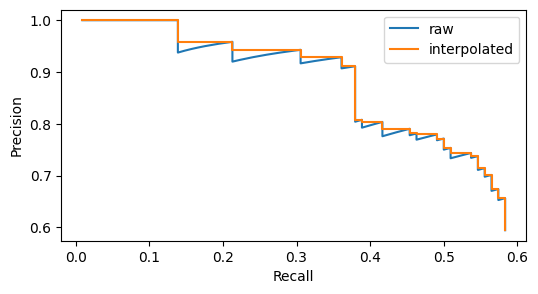
\includegraphics[height=5cm]{figs/eval/simple_mAP.png}
    \caption{\textbf{Example of an precision-recall curve.}}
    \label{fig:precision_recall}
\end{figure}

\textit{Average precision} (AP) is a summary of precision-recall trade-off, typically an estimation of the area under the curve. Following the convention of the Microsoft COCO \cite{lin_microsoft_2015} data set, AP is defined as the mean of interpolated precision sampled at 101 evenly spaced recall values:

\begin{align}
    \text{AP} &= \frac{1}{101} \sum\limits_{r\in \{0.00, 0.01, \dots, 1.00\}} \text{Precision}_{int}(r)
\end{align}

Where $\text{Precision}_{int}(r)$ is the maximum precision that corresponds to a recall value of $r$ or greater:

\begin{align}
    \text{Precision}_{int}(r) = \max\limits_{r' \geq r} \text{Precision}(r')
\end{align}

\textit{Average precision} (AP) is calculated for every class in the dataset, the mean average precision (mAP) is the unweighted mean of AP across all classes. 

\subsection{Mean Intersection over Union} \label{section:explain_miou}
Mean Intersection over Union (mIoU) measures the performance of bounding box detection. 

\textit{Intersection over Union} (IoU) between two bounding boxes is defined by the ratio of their overlapping area to their combined area:
\begin{align}
    \text{IoU}(A, B) = \frac{A \cap B}{A \cup B}
\end{align}

Generalising this for multiple boxes, I calculated the IoU for a class in the dataset by taking the sum of the intersection between all predicted bounding boxes and all ground truth bounding boxes of the class across all images, then divide this by the sum of the union between the two set of boxes. 

Similarly to mean average precision (mAP), mean intersection over union (mIoU) is the mean intersection over union (IoU) values across all classes.

mIoU  is a rarely referenced metric for which I could not find a credible definition. Without an alternative, I contacted Garðar Ingvarsson about how he derived this metric in his project \cite{ingvarsson_deep-sea_2022}, to which he replied that he experienced the same problem and proposed his own definition. In the interest of consistency, this project also followed that definition.

\section{Methodology}
In this section, I evaluate four models trained for this project. The models range over two variants of EfficientDet\cite{tan_efficientdet_2020}: EfficientDet-D0 and EfficientDet-D2. For each variant, one model is trained with supervised contrastive loss (as proposed in section \ref{section: final supcon loss} , the other is trained without. 

To ensure testing is performed on unseen data, all four models were tuned for hyperparameter and trained using 80\% of the entire dataset (train set), then tested on the remaining 20\% (test set). The same 80/20 split is used for all four models. All four models were tuned for hyperparameters independently to ensure a fair ground of comparison, and the best parameters derived for each model were used for training. 
In each epoch during training, all models were trained on the entire training dataset. After each epoch, the models were evaluated for mAP and mIoU values using the test set. Training automatically terminates if the mAP value failed to improve in 5 epochs (the mIoU value was not used due to its tendency to fluctuate significantly), which occurred within 30 epochs for all four models.

During testing, calculating just one mAP and just one mIoU value for the entire test set would not reveal their distribution of mAP and mIoU values in different examples in the test set. Instead, I applied the bootstrap technique where I randomly sampled 2000 subsets, each constituting 20\% to 40\% of the test set, and calculated mAP and mIoU independently for each one. The collected values reflect the probability distribution of the metrics and allowed me to derieve confidence interval over their values. For this project, I used the 95\% confidence interval which lies between the 2.5 and 97.5 percentile of the collected data. Figure \ref{fig:d2_spread} shows the confidence interval for 

\begin{figure}[H]
    \centering
    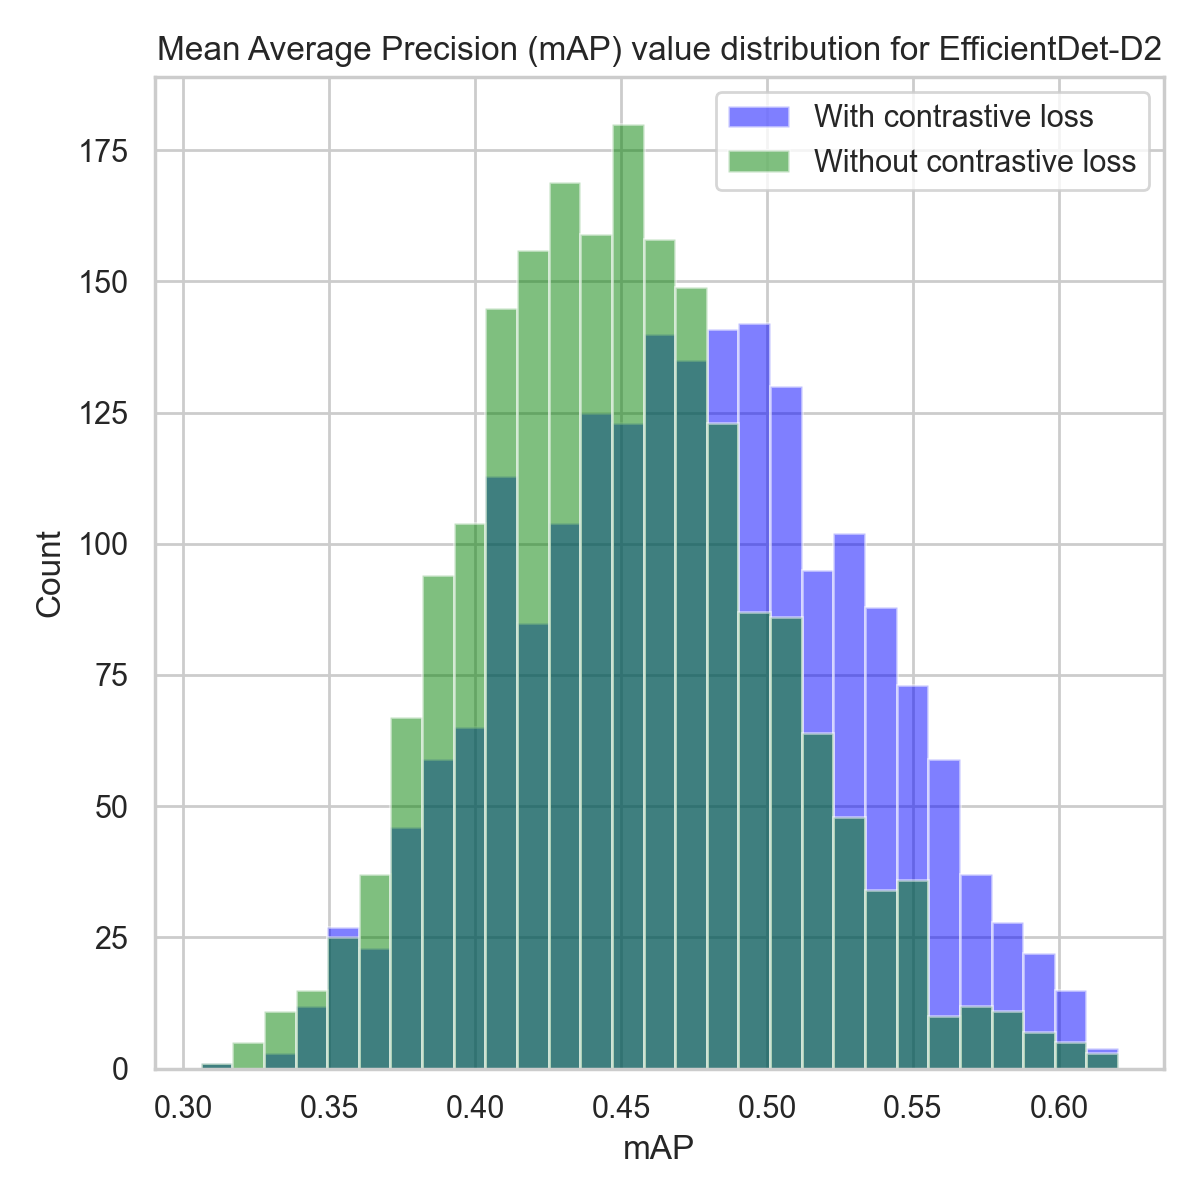
\includegraphics[width=0.48\textwidth]{figs/eval/results/d2_map_spread.png}
    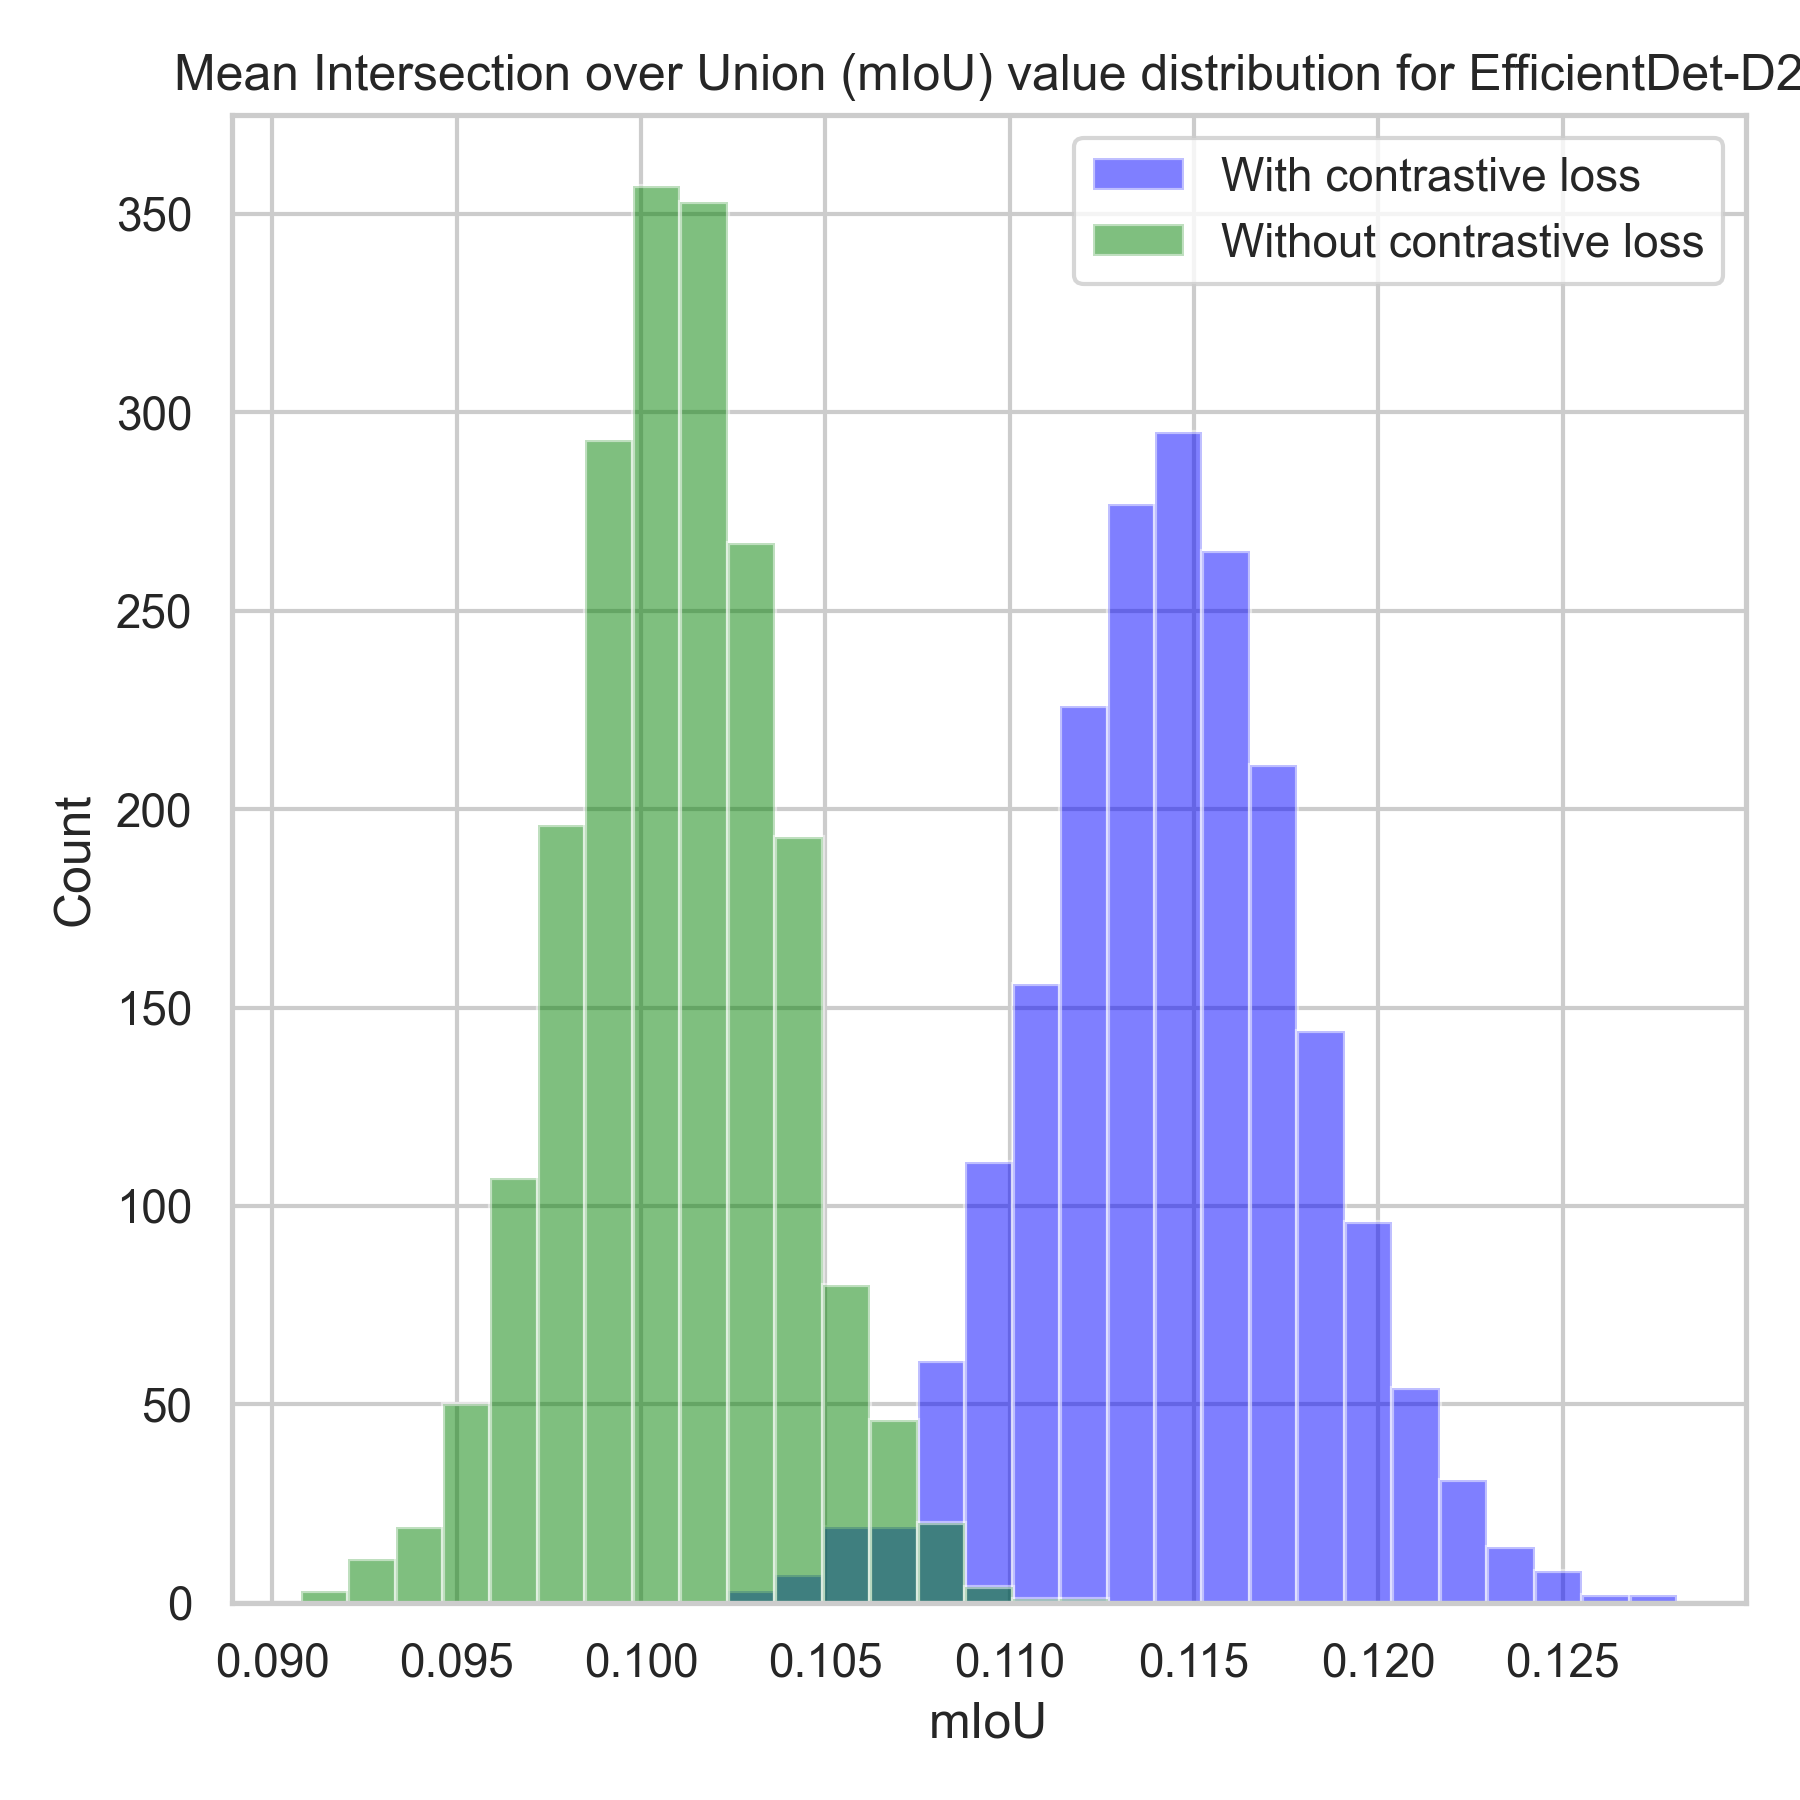
\includegraphics[width=0.48\textwidth]{figs/eval/results/d2_miou_spread.png}
    \caption{\textbf{Distribution of mAP and mIoU values for EfficientDet-D2}. The higher the better.}
    \label{fig:d2_spread}
\end{figure}

\section{Results} \label{section:eval_results}

\begin{table}[h]
    \centering
    \begin{tabular}{|l || c | c|}
        \hline
        \textbf{Model} & \textbf{mAP} & \textbf{mIoU}  \\
        \hline
        \hline
        EfficientDet-D0          &&\\
        without Contrastive Loss & -    & -\\
        with Contrastive Loss    & 0.429 \pm 0.095  & 0.086 \pm 0.006\\
        \hline
        \textbf{EfficientDet-D2}          &&\\
        without Contrastive Loss & 0.449 \pm 0.099  & 0.101 \pm 0.006\\
        \textbf{with Contrastive Loss}   & \textbf{0.473 \pm 0.110}  & \textbf{0.114 \pm 0.006}\\
        \hline
    \end{tabular}
    \caption{\textbf{Results of model evaluation} Showing mAP and mIoU values of models evaluated. For both metrics, the higher the better.}
    \label{table:eval_results}
\end{table}

Table \ref{table:eval_results} shows the results of model evaluations. The data shows that both EfficientDet-D0 and EfficientDet-D2 performed better in both mAP and mIoU when trained with supervised contrastive loss. Unsurprisingly, EfficientDet-D2 consistently outperformed EfficientDet-D0. Figure \ref{}

\subsection{Success Criteria}
For mAP, my best performing model achieved the success criteria of 0.55 within the 95\% error margin, achieving the success criteria. However, my results for mIoU were significantly lower than the 0.22 I set out to achieve. Intuitively, mIoU is likely to be affected by the quality of the data, as missing and incorrect annotations quickly reduce the amount of reasonable overlap between detection and annotation. My decision not to manually clean the dataset could have had a major negative impact here. However, mAP is a widely accepted metric that measures both classification and detection performance, making it more indicative of model performance.

\section{Efficiency} \label{section:efficiency}
In this section, I evaluate how well the project achieved its goal of \textit{efficient} organism detection. 

\subsection{Inference FLOPs}
A way to measure the efficiency of a deep learning model is to count the number of floating-point operations (FLOPs) needed to complete one forward pass. FLOPs is independent of hardware and is generally consistent across different implementations of the same model architecture.

I compared my EfficientDet implementations with Faster R-CNN \cite{ren_faster_2016}, a popular two-stage object detection architecture. For the latter, I used the implementation in the \verb|torchvision| library, which is officially part of the PyTorch project. Table \ref{table:flops} contains detailed measurements. 

\begin{table}[H]
    \centering
    \begin{tabular}{|l c|}
        \hline
        \textbf{Model}  &  \textbf{Inference FLOPs (billion)} \\
        \hline
        \textbf{EfficientDet-D0} & \textbf{8.5}\\
        EfficientDet-D1 & 13.6\\
        EfficientDet-D2 & 17.8\\
        EfficientDet-D3 & 31.4\\
        EfficientDet-D4 & 55.8\\
        EfficientDet-D5 & 89.7\\
        \textbf{Faster R-CNN (ResNet18)} & \textbf{137.2}\\
        EfficientDet-D6 & 153.5\\
        Faster R-CNN (ResNet50) & 183.3\\
        Faster R-CNN (ResNet101) & 250.2\\
        Faster R-CNN (VGG19) & 376.4\\
        \hline
    \end{tabular}
    \cprotect\caption{\textbf{Inference FLOPs comparison} in ascending FLOPs. All models were configured for 11 classes and tested with randomised input of dimension $(1, 3, 640, 1280)$. FLOPs measured using \verb|fvcore.nn.FlopCountAnalysis| and \verb|ptflops.get_model_complexity_info|.}
    \label{table:flops}
\end{table}

\begin{figure}
    \centering
    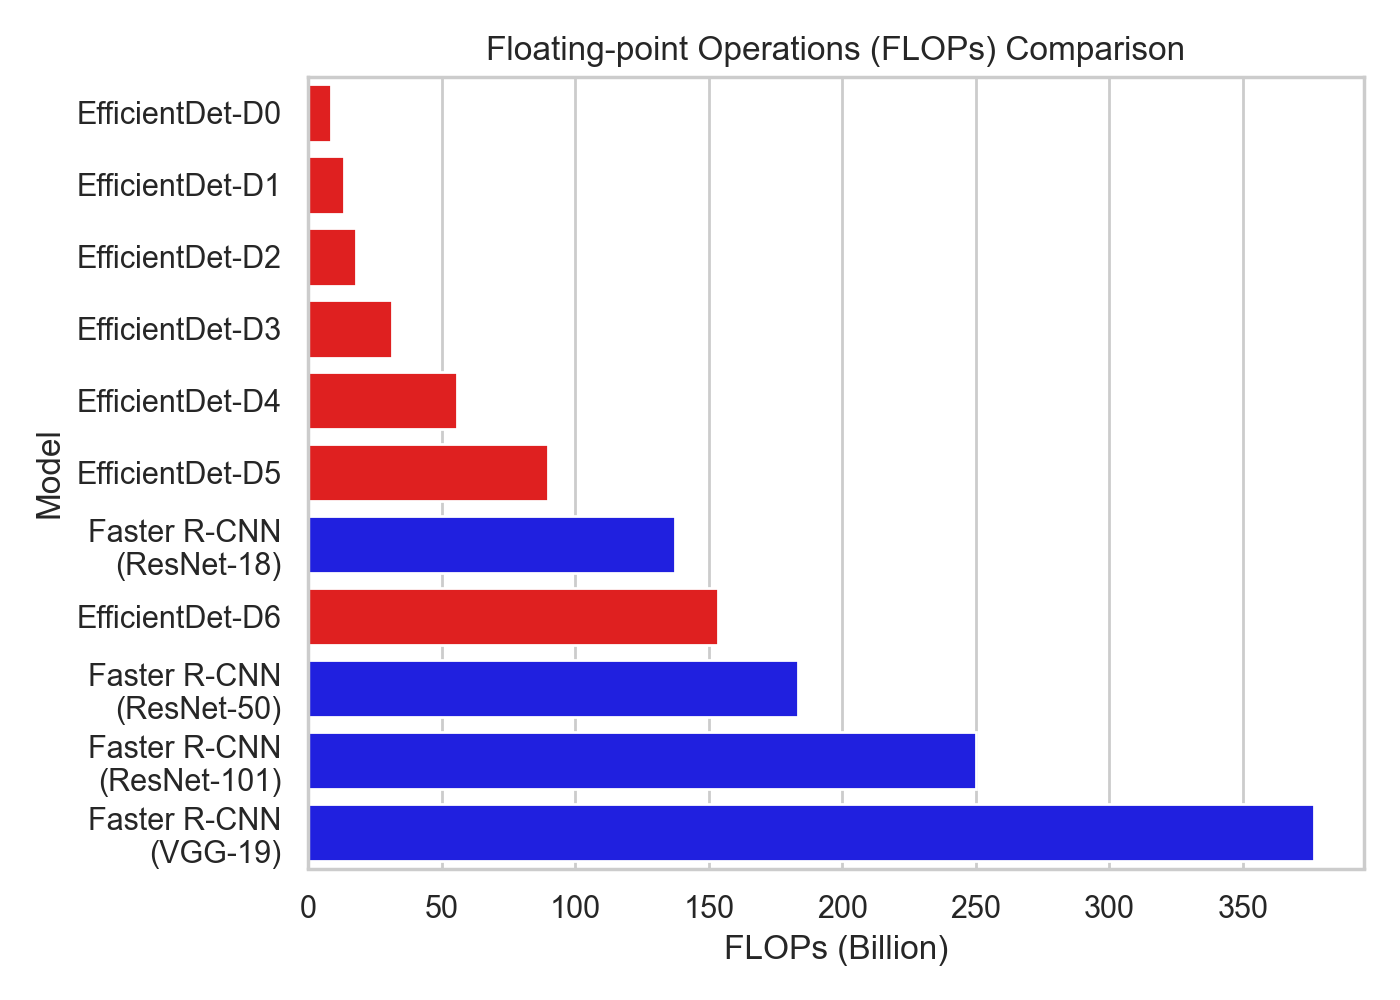
\includegraphics[width=0.8\textwidth]{figs/eval/efficiency/flops_comparisons.png}
    \caption{\textbf{Inference FLOPs comparison}}
\end{figure}

The results show that the EfficientDet models consistently require fewer FLOPs compared to Faster R-CNN models. The bigger model trained for this project, EfficientDet-D2, requires more than ten times fewer FLOPs than the smallest Faster R-CNN model. 

In general, lower FLOPs correlate with greater efficiency as fewer computations generally take less energy and time. However, FLOPs alone cannot measure inference efficiency, as it cannot account for factors such as memory access, parallelism in compute and hardware support. In real-life applications, \textit{inference latency} is often considered a more relevant metric. Inference latency refers to the time it takes for a model to produce a prediction given an input. Unlike FLOPs, inference latency varies by hardware and implementation. In the following section, I evaluate my models on inference latency.

\subsection{Inference Latency}
I measured the inference latency using my laptop, which runs a Nvidia RTX 3060 GPU (laptop variant) with 6GB of VRAM. The software setup of the system is as follows:
\vspace{5mm}

\begin{tabular}{ll}
\hline
Operating System:           & \bf Windows 11 Home (Build 22624.1755) \\
NVidia Drivers version:     & \bf 527.41 \\
CUDA Version:               & \bf   11.7.64 \\
Python Version:             & \bf 3.9.13  \\
Torch Version:              & \bf 1.13.1+cu117 \\
Torchvision Version:        & \bf 0.14.1+cu117 \\
\hline
\end{tabular}

\vspace{5mm}


When deploying machine learning models in real life, both the length and the consistency of inference latency are important considerations, so I investigated both the magnitude and the variation in my measurements. For each model, I performed 500 inferences with random examples from the dataset. To ensure that the measurements are as independent as possible from the rest of the operating system, I used \verb|Torch.cuda.Event| to accurately measure the time elapsed in the GPU. Before each set of inferences, I cleanly rebooted the laptop. The laptop was plugged in and fully charged with all power optimisations disabled. Figure \ref{fig:inference_latency} presents my measurements:

\begin{figure}[H]
    \centering
    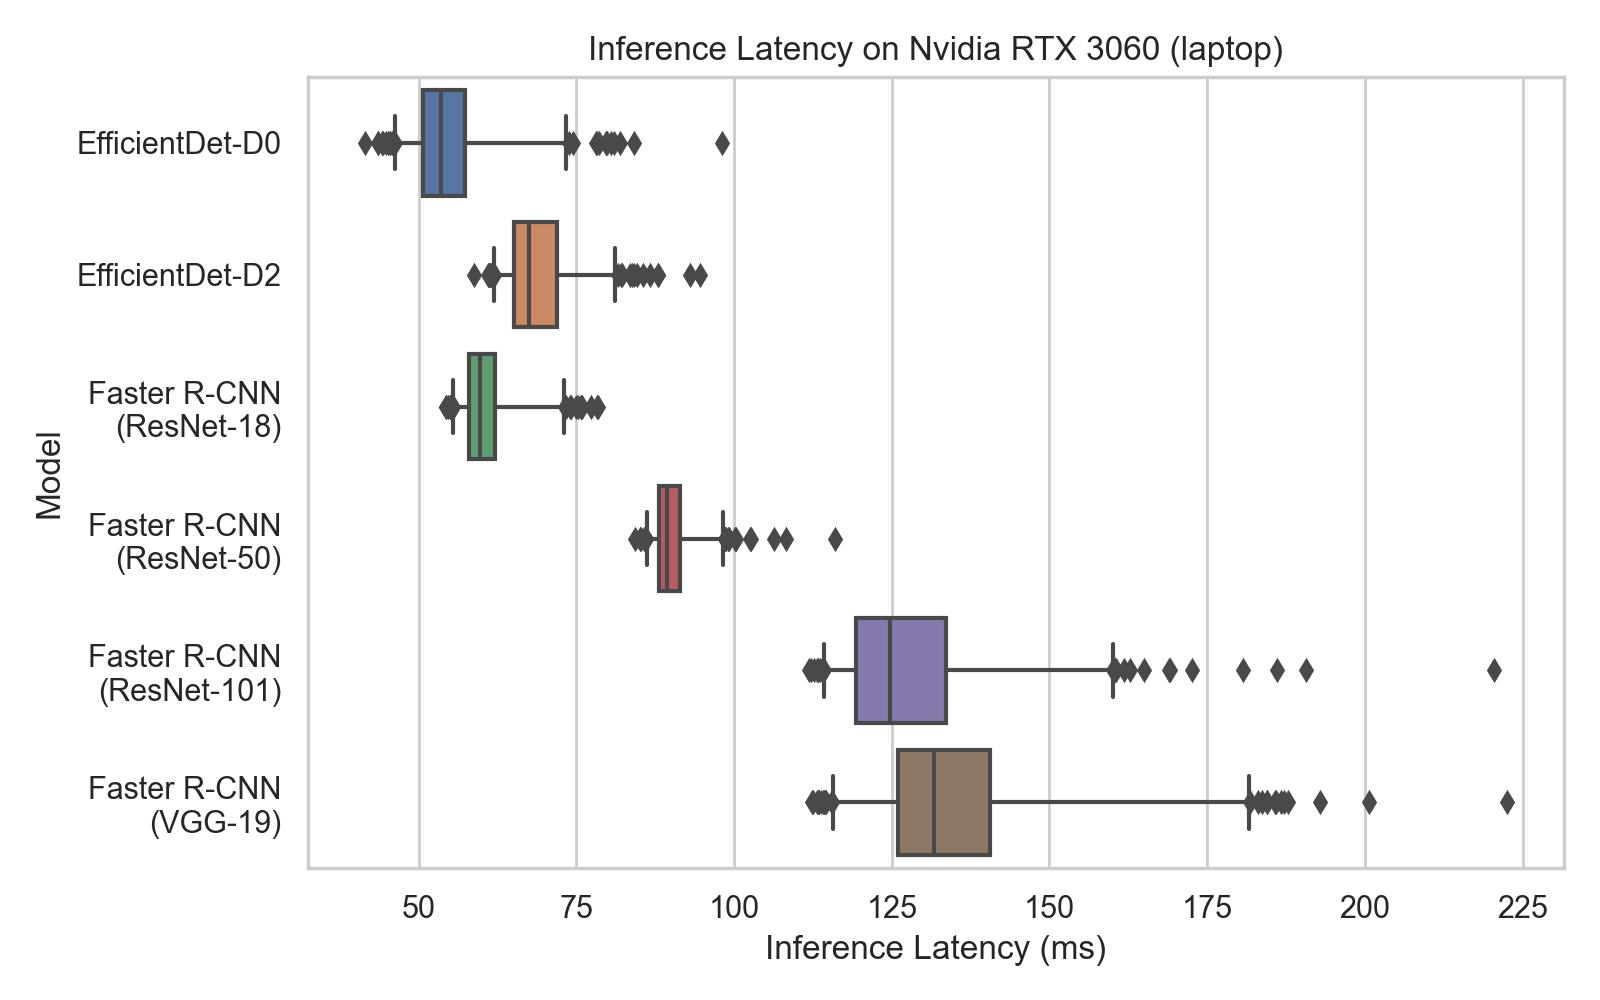
\includegraphics[width=\textwidth]{figs/eval/efficiency/inference_latency.png}
    \caption{\textbf{Inference Latency Measurements.} Each model is given 500 random inputs of marine organism, which of dimension $(1, 3, 640, 1280).$}
    \label{fig:inference_latency}
\end{figure}

Despite considerably larger FLOPs, \verb|torchvision|'s implementation of Faster R-CNN produced competitive inference latency compared to my EfficientDet. Faster R-CNN with ResNet-18 \cite{he_deep_2015} outperformed my EfficientDet-D2. The difference probably stems from a difference in implementation quality, with the official PyTorch team better at exploiting optimisations and writing efficient models. Nevertheless, my EfficientDet-D0 was the most efficient model among those compared. Achieving a 97.5 percentile latency of 73.65 ms, \textbf{ my EfficientDet-D0 should reliably produce organism detections at more than 13 frames per second (fps)}. This should be sufficient to make it useful for many applications. Improvements in hardware and hardware-specific optimisations should help further improve inference latency.  

\section{Video Detection} \label{section:video}
To see how my orgasm detection system performs, I ran the complete video orgasm detection software on two real-life underwater footage.

\subsection{Johnston Atoll}
The first footage was recorded in Johnston Atoll, a small uninhabited island near Hawaii. The footage consists mainly of close-up shots of marine creatures. The model performed well for this video, successfully detection and classifying the creature in the frame (Figure \ref{fig:johnton_good}). The model was struggling with sea eel, a creature it had not encountered before (Figure \ref{fig:johnton_bad}).

\begin{figure}[H]
    \centering
    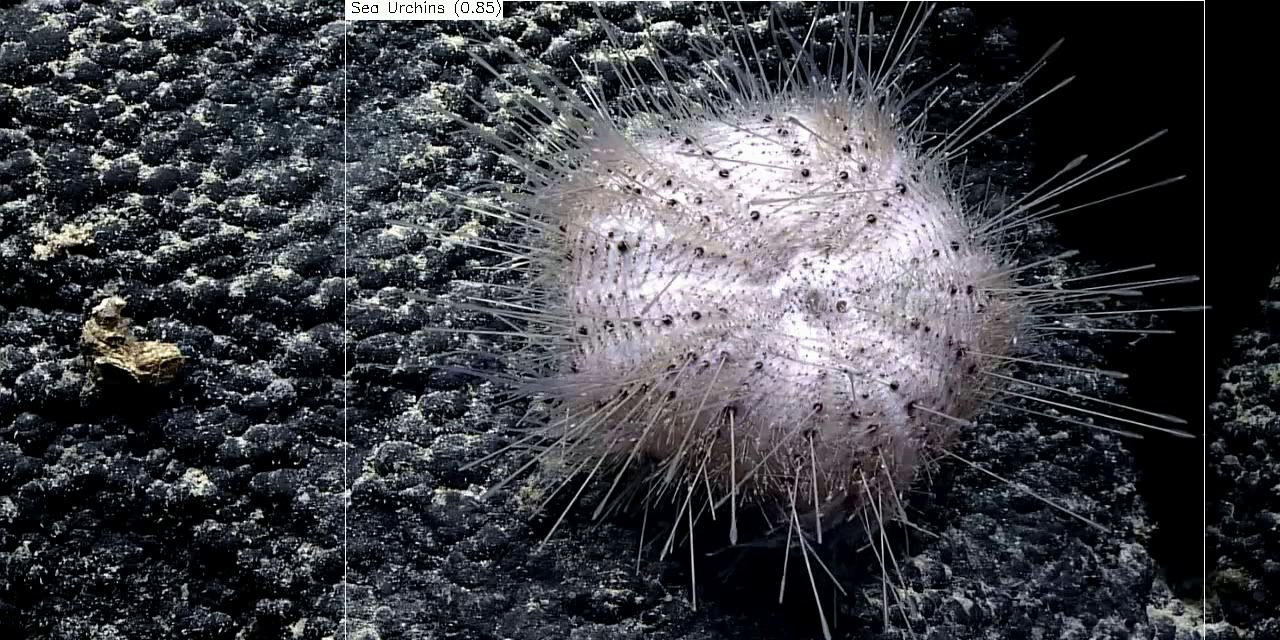
\includegraphics[width=0.75\textwidth]{figs/eval/video/johntson/urchin.png}
    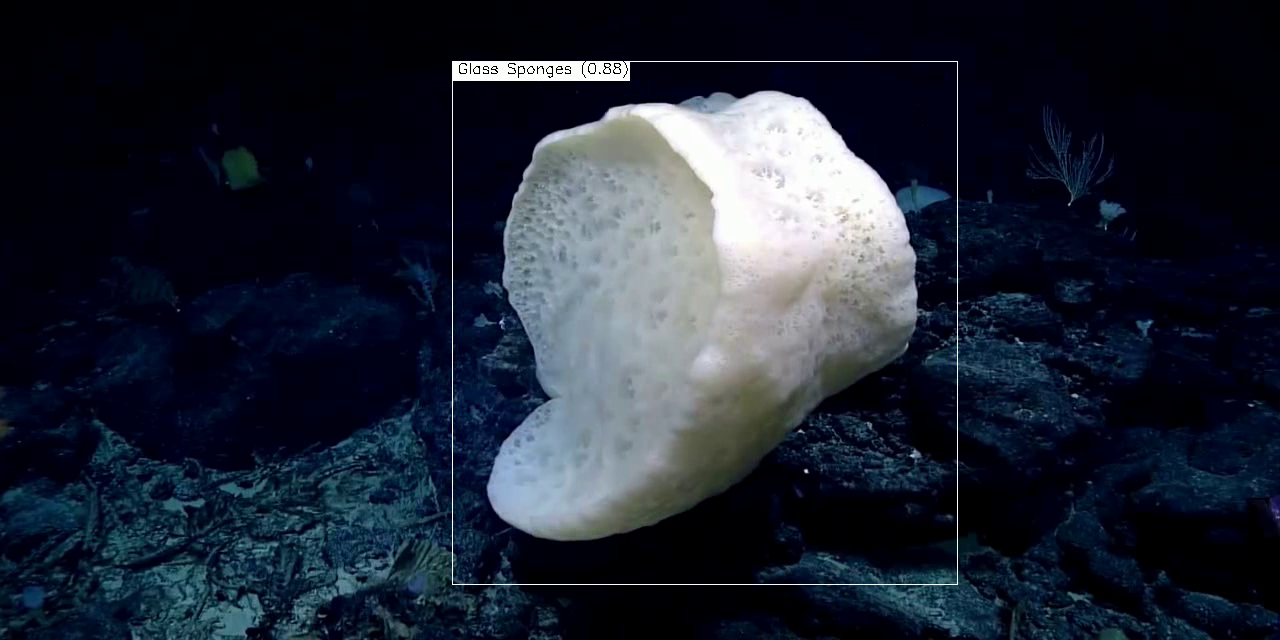
\includegraphics[width=0.75\textwidth]{figs/eval/video/johntson/glass_sponge.png}
    \caption{The model correctly localised and classified the creatures in the footage.}
    \label{fig:johnton_good}
\end{figure}
\begin{figure}[H]
    \centering
    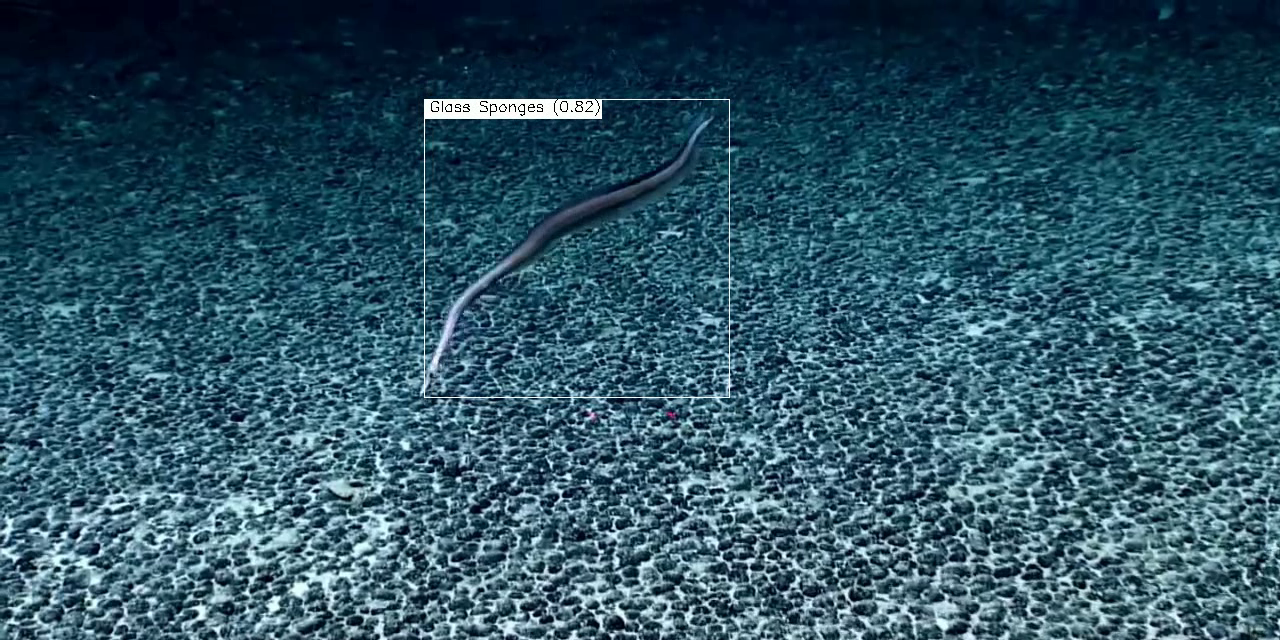
\includegraphics[width=0.75\textwidth]{figs/eval/video/johntson/snake.png}
    \caption{The model wrongly classified an eel as a glass sponge. }
    \label{fig:johnton_bad}
\end{figure}

\subsection{Forest of the Weird}
The second footage was captured in a patch on the Pacific Ocean floor nicknamed the ``forest of the weird'' due to the many exotic glass sponges that live there. With many creatures captured in each frame, this video presents a more challenging example for the model. Nonetheless, the model was able to correctly localise and classifier creatures in the footage. (Figure \ref{fig:forest1})

\begin{figure}[H]
    \centering
    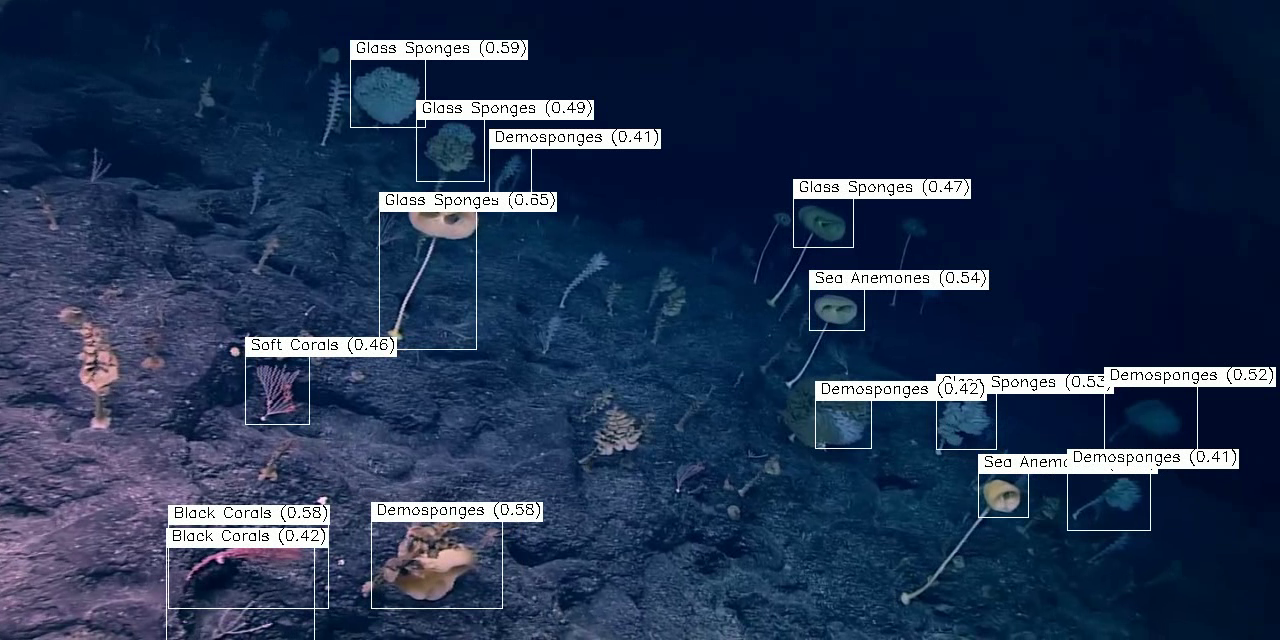
\includegraphics[width=0.75\textwidth]{figs/eval/video/forest/good.png}
    \caption{The model functioned well despite the high number of creatures in the scene, including small annotations like soft coral.}
    \label{fig:forest1}
\end{figure}


\chapter{Conclusions}

\section{Accomplishments}
The project achieved its core objective of delivering an efficient software to detect deep-sea marine organisms. The delivered software offers competitive inference latency and produced good results on real-world footage. In the process, 

The project also proposed and implemented a supervised contrastive learning technique for object detection, representing one of the pioneering research effort in the field. The project also created a dynamic training example generator which 


%%%%%%%%%%%%%%%%%%%%%%%%%%%%%%%%%%%%%%%%%%%%%%%%%%%%%%%%%%%%%%%%%%%%%
% the bibliography
\printbibliography[
heading=bibintoc,
title={Bibliography}
]

%%%%%%%%%%%%%%%%%%%%%%%%%%%%%%%%%%%%%%%%%%%%%%%%%%%%%%%%%%%%%%%%%%%%%
% the appendices
\appendix


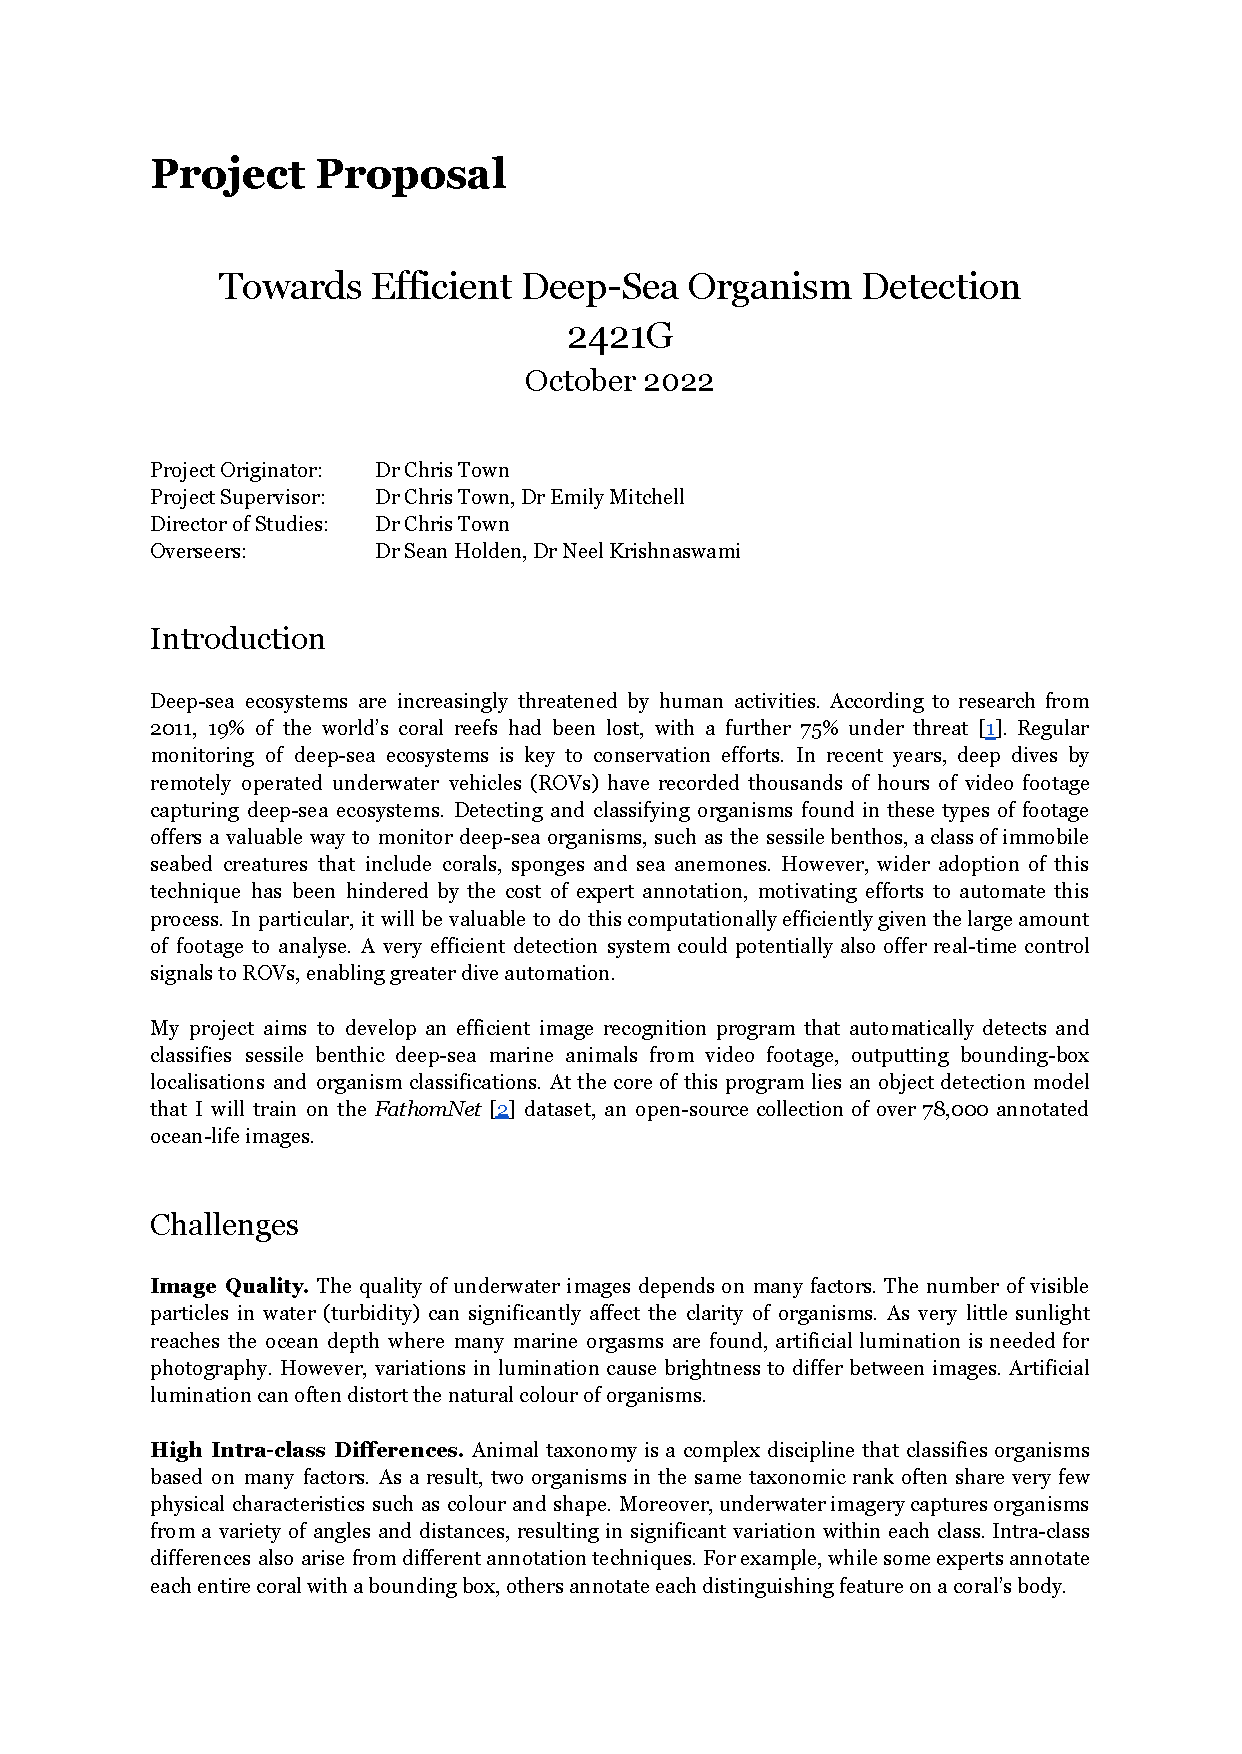
\includepdf[pages=-, addtotoc={
     1,chapter,1,Project Proposal,p1,   
     1,section,1,Introduction,p2,
     1,section,1,Challenges,p3,
     2,section,1,Related Works,p4,
     2,section,1,Project Methodology,p5,
     3,section,1,Project Structure,p6,
     4,section,1,Success Criteria,p7,
     4,section,1,Starting Point,p8,
     4,section,1,Resources Required,p9,
     5,section,1,Timetable and Milestones,p10}]
     {proposal.pdf}

\end{document}